% Template for the submission to:
%   The Annals of Applied Statistics    [AOAS]
%
%%%%%%%%%%%%%%%%%%%%%%%%%%%%%%%%%%%%%%%%%%%%%%
%% In this template, the places where you   %%
%% need to fill in your information are     %%
%% indicated by '???'.                      %%
%%                                          %%
%% Please do not use \input{...} to include %%
%% other tex files. Submit your LaTeX       %%
%% manuscript as one .tex document.         %%
%%%%%%%%%%%%%%%%%%%%%%%%%%%%%%%%%%%%%%%%%%%%%%

\documentclass[aoas]{imsart}

%% Packages
\RequirePackage{amsthm,amsmath,amsfonts,amssymb,centernot,float,import,makeidx,subfiles}
\RequirePackage{natbib}
%\RequirePackage[colorlinks,citecolor=blue,urlcolor=blue]{hyperref}
\RequirePackage{graphicx}% uncomment this for including figures

\startlocaldefs
%%%%%%%%%%%%%%%%%%%%%%%%%%%%%%%%%%%%%%%%%%%%%%
%%                                          %%
%% Uncomment next line to change            %%
%% the type of equation numbering           %%
%%                                          %%
%%%%%%%%%%%%%%%%%%%%%%%%%%%%%%%%%%%%%%%%%%%%%%
%\numberwithin{equation}{section}
%%%%%%%%%%%%%%%%%%%%%%%%%%%%%%%%%%%%%%%%%%%%%%
%%                                          %%
%% For Axiom, Claim, Corollary, Hypothezis, %%
%% Lemma, Theorem, Proposition              %%
%% use \theoremstyle{plain}                 %%
%%                                          %%
%%%%%%%%%%%%%%%%%%%%%%%%%%%%%%%%%%%%%%%%%%%%%%
%%%%%%%%%%%%%%%%%%%%%%%%%%%%%%%%%%%%%%%%%%%%%%
\theoremstyle{plain}
\newtheorem{axiom}{Axiom}
\newtheorem{claim}[axiom]{Claim}
\newtheorem{theorem}{Theorem}[section]
\newtheorem{lemma}[theorem]{Lemma}
\newtheorem{proposition}{Proposition}
\newcommand{\matr}[1]{\mathbf{#1}} % undergraduate algebra version

%%%%%%%%%%%%%%%%%%%%%%%%%%%%%%%%%%%%%%%%%%%%%%
%%                                          %%
%% For Assumption, Definition, Example,     %%
%% Notation, Property, Remark, Fact         %%
%% use \theoremstyle{remark}                %%
%%                                          %%
%%%%%%%%%%%%%%%%%%%%%%%%%%%%%%%%%%%%%%%%%%%%%%
\theoremstyle{remark}
\newtheorem{remark}{remark}
%%%%%%%%%%%%%%%%%%%%%%%%%%%%%%%%%%%%%%%%%%%%
%\theoremstyle{plain}
%\newtheorem{???}{???}
%\newtheorem*{???}{???}
%\newtheorem{???}{???}[???]
%\newtheorem{???}[???]{???}
%%%%%%%%%%%%%%%%%%%%%%%%%%%%%%%%%%%%%%%%%%%%%%
%%                                          %%
%% For Assumption, Definition, Example,     %%
%% Notation, Property, Remark, Fact         %%
%% use \theoremstyle{remark}                %%
%%                                          %%
%%%%%%%%%%%%%%%%%%%%%%%%%%%%%%%%%%%%%%%%%%%%%%
%\theoremstyle{remark}
%\newtheorem{???}{???}
%\newtheorem*{???}{???}
%\newtheorem{???}{???}[???]
%\newtheorem{???}[???]{???}
%%%%%%%%%%%%%%%%%%%%%%%%%%%%%%%%%%%%%%%%%%%%%%
%% Please put your definitions here:        %%
%%%%%%%%%%%%%%%%%%%%%%%%%%%%%%%%%%%%%%%%%%%%%%

\endlocaldefs

\begin{document}

\begin{frontmatter}
%%%%%%%%%%%%%%%%%%%%%%%%%%%%%%%%%%%%%%%%%%%%%%
%%                                          %%
%% Enter the title of your article here     %%
%%                                          %%
%%%%%%%%%%%%%%%%%%%%%%%%%%%%%%%%%%%%%%%%%%%%%%
\title{The Effect of Medicaid Expansion on Non-Elderly Adult Uninsurance Rates Among States that did not Expand Medicaid}
%\title{A sample article title with some additional note\thanksref{T1}}
\runtitle{}
%\thankstext{T1}{A sample of additional note to the title.}

\begin{aug}
%%%%%%%%%%%%%%%%%%%%%%%%%%%%%%%%%%%%%%%%%%%%%%
%%Only one address is permitted per author. %%
%%Only division, organization and e-mail is %%
%%included in the address.                  %%
%%Additional information can be included in %%
%%the Acknowledgments section if necessary. %%
%%%%%%%%%%%%%%%%%%%%%%%%%%%%%%%%%%%%%%%%%%%%%%
\author[A]{\fnms{Max} \snm{Rubinstein}\ead[label=e1]{Heinz College and Department of Statistics and Data Science}} and
\author[A]{\fnms{Amelia} \snm{Haviland}\ead{Heinz College and Department of Statistics and Data Science}}
%%%%%%%%%%%%%%%%%%%%%%%%%%%%%%%%%%%%%%%%%%%%%%
%% Addresses                                %%
%%%%%%%%%%%%%%%%%%%%%%%%%%%%%%%%%%%%%%%%%%%%%%
\address[A]{Carnegie Mellon University, \printead{e1}}

\end{aug}

We estimate the effect of Medicaid expansion on the adult uninsurance rate in states that did not expand Medicaid in 2014. Using data from the American Community Survey (ACS), we estimate this effect - the treatment effect on the controls (ETC) - by re-weighting expansion regions to approximately balance the covariates from non-expansion regions using an extension of the stable balancing weights objective function (\cite{zubizarreta2015stable}). We contribute to the balancing weights literature by accounting for hierarchical data structure and covariate measurement error when calculating our weights, and to the synthetic controls literature (see, e.g. \cite{abadie2010synthetic}) by outlining a set of assumptions that identifies the ETC using time-series cross-sectional data. We estimate that Medicaid expansion would have changed the uninsurance rate by -2.33 percentage points (-3.49, -1.16). These results are smaller in absolute magnitude than existing estimates of the treatment effect on the treated (ETT), though may not be directly comparable due to the study design, target population, and level of analysis. Regardless, we caution against making inferences about the ETC using estimates of the ETT, and emphasize the need to directly estimate the appropriate counterfactual when they are the quantity of interest.



\begin{keyword}
\kwd{Synthetic controls}
\kwd{balancing weights}
\kwd{medicaid expansion}
\kwd{measurement error}
\kwd{hierarchical data}
\kwd{regression to the mean}
\end{keyword}

\end{frontmatter}
%%%%%%%%%%%%%%%%%%%%%%%%%%%%%%%%%%%%%%%%%%%%%%
%% Please use \tableofcontents for articles %%
%% with 50 pages and more                   %%
%%%%%%%%%%%%%%%%%%%%%%%%%%%%%%%%%%%%%%%%%%%%%%
%\tableofcontents

%%%%%%%%%%%%%%%%%%%%%%%%%%%%%%%%%%%%%%%%%%%%%%
%%%% Main text entry area:

\section{Introduction}
\input{03_Paper/01-introduction-alt}

\section{Data}
In this section we provide an overview of our data source, the covariates, the outcome, and the treatment assignment.

\subsection{Data Source}

Our primary data source is the annual household and person public use microdata files from the American Community Survey (ACS) from 2011 through 2014. The ACS is an annual survey of approximately three million individuals across the United States. The public use microdata files include information on individuals in geographic areas greater than 65,000 people. The smallest geographic unit contained in these data are public-use microdata areas (PUMAs), arbitrary boundaries that nest within states but not within counties or other more commonly used geographic units. One limitation of these data is a 2012 change in the PUMA boundaries, which do not overlap well with the previous boundaries. As a result, the smallest possible geographic areas that nest both PUMA coding systems are known as consistent PUMAs (CPUMAs). The United States contains 1,075 total CPUMAs, with states ranging from having one CPUMA (South Dakota, Montana, and Idaho) to 123 CPUMAs (New York). Our primary dataset (discussed in Section~\ref{sssec:txassign} contained 929 CPUMAs among 46 states. The average total number of sampled individuals per CPUMA across the four years is 1,001; the minimum number of people sampled was 334 and the maximum is 23,990. Importantly, this survey is a repeated cross-section rather than a longitudinal dataset of individuals over time.

\subsection{Study period}

We begin our analysis in 2011 following \cite{courtemanche2017early}, who note that several other aspects of the ACA were implemented in 2010 -- including the provision allowing for dependent coverage until age 26 and the elimination of co-payments for preventative care -- and likely induced differential shocks across states. We also restrict our post-treatment period to 2014: several additional states expanded Medicaid in 2015, including Indiana, Michigan, and Pennsylvania. However, these states did not expand Medicaid contemporaneously with the 2014 ACA provisions. Without additional assumptions, this second-year expansion cannot help us estimate the effect of the 2014 expansion. 

\subsection{Covariates}

We use the underlying individual-level ACS survey data and accompanying survey weights to aggregate the data at the CPUMA level. We choose our covariates to approximately align with those considered in \cite{courtemanche2017early} and that are likely to be potential confounders. Because we are ultimately interested in calculating rates, these variables include both the numerator and denominator counts.

Using the ACS survey weights, we first estimate: the total non-elderly adult population for each year 2011-2014; the total labor force population (among non-elderly adults) for each year 2011-2013; and the total number of households averaged from 2011-2013. We also construct an average of the total non-elderly adult population from 2011-2013. These are our denominator variables. For our numerator counts, we estimate the total number of: females; whites; people of Hispanic ethnicity; people born outside of the United States; citizens; people with disabilities; married individuals; people with less than a high school education, high school degrees, some college, or college graduates or higher; people living under 138 percent of the FPL, between 139 and 299 percent, 300 and 499 percent, more than 500 percent, and who did not respond to the income survey question; people aged 19-29, 30-39, 40-49, 50-64; households with one, two, or three or more children, and households that did not respond about the number of children.\footnote{Number of children and income to poverty ratio were the only two variables with missing data in the underlying microdata.} We average these estimated counts using the ACS survey weights from 2011-2013. For each individual year from 2011-2013, we estimate the total number of people who were unemployed and uninsured at the time of the survey (calculated among all non-elderly adults and all non-elderly adults within the labor force, respectively). We divide the numerator counts by the corresponding denominator counts to estimate the percentage in each category. For the demographics, these include the average number of non-elderly adults from 2011-2013. For the time-varying variables, we use the corresponding year (where uninsurance rates are calculated as a fraction of the labor force rather than the non-elderly adult population). We also calculate the average non-elderly adult population growth and the average number of households to adults across 2011-2013. 

In addition to the ACS microdata, we use 2010 Census data to calculate the approximate percentage of people living within an ``urban'' area for each CPUMA. Finally, we include three state-level covariates reflecting the partisan composition of each state's government in 2013 using data from the National Conference of State Legislatures (NCLS). Specifically, we generate an indicator for states with a Republican governor, an indicator for states with Republican control over the lower legislative chamber, and an indicator for states with Republican control over both chambers of the legislature and the governorship.\footnote{Nebraska is the only state with a unicameral legislature; moreover, the legislature is technically non-partisan. We nevertheless classified them as having Republican control of the legislature.} 

\subsection{Outcome}

Our outcome of interest is the non-elderly adult uninsurance rate in 2014, which we denote using $Y$. While take-up among the Medicaid-eligible population is a more natural outcome, we choose the non-elderly adult uninsurance rate for two reasons, one theoretic and one practical. First, Medicaid eligibility in the post-period is likely endogenous: Medicaid expansion may affect an individual's income and poverty levels, which in general define Medicaid eligibility. A second reason is to align our study with others to compare our results with the existing literature, and this is the outcome that \cite{courtemanche2017early} use. One drawback of using this outcome is that the simultaneous adoption of other ACA provisions by all states in 2014 more clearly affects this rate in a way that a more targeted group might not be.

\subsection{Treatment assignment} \label{sssec:txassign}

While some states expanded Medicaid in 2014 and other states did not, assigning a binary treatment status simplifies a more complex reality. There are three reasons to be cautious about this simplification. First, states differed substantially in their Medicaid coverage policies prior to 2014: with perfect data we might consider Medicaid expansion as a continuous treatment with values proportional to the number of newly eligible individuals. The challenge, however, is correctly identifying newly eligible individuals in the data (see \cite{frean2017premium}, who attempt to address this). Second, \cite{frean2017premium} note that five states (California, Connecticut, Minnesota, New Jersey, and Washington) and the District of Columbia adopted partial limited Medicaid expansions prior to 2014. \footnote{\cite{kaestner2017effects} and \cite{courtemanche2017early} also consider Arizona, Colorado, Hawaii, Illinois, Iowa, Maryland, and Oregon to have had early expansions.} Lastly, timing is an issue: among the states that expanded Medicaid in 2014, Michigan's expansion did not go into effect until April 2014, while New Hampshire's expansion did not occur until September 2014.

Our primary analysis excludes New York, Vermont, Massachusetts, Delaware, and the District of Columbia from our pool of expansion regions, because these regions had comparable Medicaid coverage policies prior to 2014 (\cite{kaestner2017effects}). We also exclude New Hampshire because it did not expand Medicaid until September 2014. While Michigan expanded Medicaid in April 2014, we leave this state in our pool of treated states. We consider the remaining expansion states as ``treated'' and the non-expansion states as ``control'' states. We later consider the sensitivity of our results to these classifications by removing the early expansion states noted by \cite{frean2017premium}. Our final dataset contains aggregated statistics for all of the above variables for 925 CPUMAs in our non-expansion and our pool of expansion states. There are 414 CPUMAs among 24 non-expansion states and 511 CPUMAs among 21 expansion states. When we exclude the early expansion states for sensitivity analyses, we are left with 296 CPUMAs across 17 expansion states.

\section{Methods}\label{sec:methods}
In this section we present our causal estimand, identifying assumptions, estimation strategy, and inferential procedure.

\subsection{Estimand}

Our goal is to estimate the average effect 2014 Medicaid expansion would have had on the non-elderly adult uninsurance rate in states that did not expand Medicaid. Let $A$ indicate treatment assignment, $c$ index a CPUMA, $s$ index the state, and $t$ index the time period. Let $n_1$ be the number of treated CPUMAs, $n_0$ be the number of control CPUMAs, and $n$ be the total number of CPUMAs. Similarly, let and $m = m_1 + m_0$ states (with $m_1$ and $m_0$ defined analogously). Each state has $p_s$ CPUMAs. Since we are only interested in the counterfactual at time $T = 2014$, we simplify notation by removing this variable and the subscript and write our formal estimand as:

\begin{equation}
\psi = \psi^1 - \psi^0 &= n_0^{-1}\sum_{s, c: A_s = 0} Y_{sc}^{A_s = 1} - Y_{sc}^{A_s = 0} 
\end{equation}

The challenge is that we do not observe the counterfactual outcomes for non-expansion CPUMAs had they been in states that expanded their Medicaid programs. We therefore require causal assumptions to tie this counterfactual quantity to our observed data.\footnote{The 2014 Medicaid expansion occurred simultaneously with the implementation of several other major ACA provisions, including (but not limited to) the creation of the ACA-marketplace exchanges, the individual mandate, health insurance subsidies, and community-rating and guaranteed issue of insurance plans (\cite{courtemanche2017early}). Almost all states broadly implemented these reforms beginning January 2014. Conceptually we think of the other ACA components as a state-level treatment ($R$) separate from Medicaid expansion ($A$). Therefore, our total estimated effect may also include interactions between these policy changes; however, we do not attempt to separately identify these effects. Because the ACA implementation and Medicaid expansion may vary over time, we do not try to generalize these results beyond 2014.} 

\subsection{Identification}

The following causal assumptions are necessary (though insufficient) to identify our target parameter from our observed data: the stable unit treatment value assumption (SUTVA), no unmeasured confounding, and no anticipatory treatment effects. We explain these assumptions in detail and their consequences below. We additionally invoke several parametric assumptions to help us identify our causal parameter given the measurement error in our covariates. These assumptions in total are sufficient to identify our causal estimand.

SUTVA has two implications: first, that there is only one version of treatment; second, that $Y_{sc}^{\mathbf{a}} = Y_{sc}^{\mathbf{a}'}$ when $a_{sc} = a_{sc}'$, where $\mathbf{a}$ is the vector of all treatment assignments. We discussed potential violations of the first assumption previously when considering how to reduce Medicaid Expansion to a binary treatment classification. Our solution is to remove states with less restrictive Medicaid eligibility requirements prior to 2014 to approximately satisfy this condition. The second part of this assumption implies that the potential outcomes in each region do not depend on another region's treatment assignment. This is a standard assumption, but is often not realistic in practice. Violations are likely in our setting: for example, \cite{frean2017premium} find evidence that Medicaid expansion drove previously eligible but uninsured individuals to enroll in Medicaid in both expansion and non-expansion states. Signing the potential bias from this violation requires redefining the causal estimand: for example, we might consider the treatment effect on the untreated given that all states have expanded Medicaid, where the contrast is against where only the observed expansion states expanded Medicaid. If the spillover effects were equal in each region, and the magnitude of the spillovers increase with the total number of treated regions, then the true effect would be larger in absolute magnitude than the estimated estimand using the observed data. We could consider other estimands or assumptions to get different predictions about the sign of the bias; however, this is beyond the scope of this paper.

We next assume that there were no anticipatory treatment effects. Letting treatment occur at time $T$, we have that for $t < T$:

\begin{align*}
Y_{sct} = Y_{sct}^0
\end{align*}

This assumption is necessary because we will condition on pre-treatment outcomes. If these outcomes were affected by the treatment before it were implemented, these covariates would be endogenous. Anticipatory treatment effects may occur if plans to expand Medicaid induce uninsured but Medicaid-eligible individuals to enroll in Medicaid prior to expansion. We do not think these violations occurred in large enough numbers to substantially affect our results. Instead, we address a more concerning version of this violation: the fact that several states allowed certain counties to expand Medicaid prior to 2014. We test the sensitivity of our results to the exclusion of these states.

Third, we assume no unmeasured confounding; that is, that at time $T$ the potential outcomes for each CPUMA are independent of the state-level treatment assignment conditional on the population-level CPUMA and state-level covariates $X_{sc}$, a $q$ dimensional vector of covariates (which includes pre-treatment outcomes):

\begin{align*}
Y_{sc}^a \perp A_{sc} \mid X_{sc}
\end{align*}

While unverifiable, we believe it is reasonable here given our rich covariate set. To be explicit, we believe that the potential uninsurance rates for each CPUMA are independent of the treatment assignment conditional on the percentage of uninsured individuals in each year of the pre-treatment period, the percentage of unemployed individuals in each year of the pre-treatment period, the average population growth, the average ratio of households to non-elderly adult population, the state's political composition, the average proportion of households with one, two, or three or more children during the pre-treatment period, the average proportion of households who did not respond about their number children, and the average proportion of individuals during the pre-treatment period with given demographics noted above (age group, sex, white, Hispanic ethnicity, U.S. citizenship, foreign born, income-to-poverty group (including non-response), disability status, urban residence, and educational attainment group). 

A key problem we address in this paper is the violation of this assumption due to measurement error in our covariates. Let 
$\matr{X} = \begin{matrix}
\matr{X}_0\\
\matr{X}_1
\end{matrix}$ be the $n$ by $q$ matrix of true covariates (and separating the control from treated units using $\matr{X}_a$) and define $\matr{W}$ analogously. Because our covariates are estimated using the ACS data, rather than $(Y, \matr{X})$, we instead observe $(J, \matr{W})$, which consist of estimates of the true covariate values. Importantly, $Y_{sc}^a \perp A_{sc} \mid X_{sc} \centernot\implies J_{sc}^a \perp A_{sc} \mid W_{sc}$. The use of these proxies may therefore bias our estimates. We rely on several modeling assumptions to correct for this.

We first model our observed data as functions of the true values plus mean-zero Gaussian noise: $J_{sc} = Y_{sc} + \xi_{sc}$ and $W_{sc} = X_{sc} + v_{sc}$, where we assume $\xi_{sc}$ and $v_{sc}$ are independent though not identically distributed.\footnote{Our covariates are almost all ratio estimates, which will in general be biased. This bias, however, decreases quickly with the sample size (is $O(n^{-1})$). Given that our CPUMA sample sizes are all over 300, we treat these estimates as unbiased in our analysis.} We assume that these errors are uncorrelated with the true values, i.e. $\mathbb{E}\{\xi_{sc} \mid Y_{sc}\} = 0$ (and similarly for all elements of $X$). Second, we assume that $\xi_{sc}$ are uncorrelated with the errors in the covariate measurements. These assumptions and our model for the observed data are reasonable given that the measurement error in this context is sampling variability. Moreover, our outcomes are measured on a different cross-section than our covariates, so it is reasonable to assume that they are uncorrelated with the measurement errors in the covariates. 

We next assume that the true potential outcomes are linear in the true covariates $X_{sc}$. Specifically, we assume that the following model generates the potential non-elderly adult uninsurance rate under treatment $A = a$:

\begin{equation}\label{eqn:outcomemodel}
Y_{sc}^a = \alpha_a + X_{sc}^T\beta_a + \epsilon_{sc} + c_s
\end{equation}

We assume that the errors $\epsilon_{sc}$ and $c_s$ are mean-zero, independent from each other and across time (i.e., we rule out serial-correlation), and are uncorrelated with the true covariates and the treatment assignment $\mathbb{E}\{\epsilon_{sc} \mid X_{sc}, A_s\} = \mathbb{E}\{c_s \mid X_{sc}, A_s\} = 0$. We can then identify $\psi^a$ in terms of our model parameters (see Appendix A); specifically, we have that $\psi^a = \alpha_a + \bar{X}_0^T\beta_a$, where $\bar{X}_0$ is the vector of mean covariate values among the control units. Moreover, we can substitute $J_{sc}$ for $Y_{sc}$ in Equation~\ref{eqn:outcomemodel}, and add $\xi_{sc}$ to the error term without affecting identification. 

We still have the problem that we observe $W_{sc}$ instead of $X_{sc}$. Let $\eta_a = \mathbb{E}\{X_{sc} \mid W_{sc}, A_s = a\}$. By linearity, we know that

\begin{equation}
    J_{sc} = \eta_a(W_{sc})^T\beta + (X_{sc} - \eta_a(W_{sc}))^T\beta + \xi_{sc} + \epsilon_{sc} + c_s 
\end{equation}

If we knew $\eta_a$, we could estimate this model using the observed data $(J, \matr{W})$. The approach we follow here is known as ``regression calibration'' in the measurement-error literature. In particular, we assume a linear model for $\eta_a$:

\begin{align*}
\eta_a(W_{sc}) = \upsilon_a + \kappa_a^T(W_{sc} - \upsilon_a)
\end{align*}

where $\kappa_a = (\Sigma_{XX \mid A = a} + \Sigma_{vv \mid A = a})^{-1}\Sigma_{XX \mid A = a}$. This assumptions motivating this model is that $(X_{sc}, v_{sc}) \stackrel{iid}\sim MVN((\upsilon_a, 0), \Sigma_a)$ and $\Sigma_a$ is a $2q$ by $2q$ block-diagonal matrix consisting of $q$ by $q$ matrices $\Sigma_{XX \mid A = a}$ and $\Sigma_{vv \mid A = a}$ and $0$ in the off-diagonals. Given sufficient auxillary data to estimate $\kappa_a$, we can then estimate $\psi$. We discuss this further below and in Appendices A and B (see also \cite{gleser1992importance}).

\subsection{Estimation}

We outline our estimation strategy first emphasizing how estimating the ETC differs from estimating the ETT with respect to variable selection under the ``synthetic controls'' framework. Second, we explain our estimation procedure, whicht modifies the SBW criterion to address the hierarchical data structure (which we call H-SBW) that reduces the variance of our estimator under our assumption of constant variance and constant within-state correlation of model errors. Third, we connect our estimator to the regression calibration literature by generating weights that balance a linear prediction of the true covariates $\hat{\eta}_a(W_{sc})$ using the observed covariates $W_{sc}$. Fourth, we test the sensitivity of our estimator to a regression-augmented version, using ridge-regression weights following the suggestion of \cite{ben2018augmented}; this allows us to achieve better covariate balance by extrapolating beyond the support of the data. We conclude by proposing a model validation procedure that uses pre-treatment outcomes to compare the performance of our estimators on pre-treatment data.

\subsubsection{Variable selection}

We seek to generate a set of positive weights that balance the means of covariates for the treated units to the mean covariates for the control units. Assume that we observe the true covariate matrices for the treated data $\matr{X}_1 = (X_{1,1}, ..., X_{1, q})$, $\matr{X}_0$ (defined similarly), and the true outcomes $Y$. Let $\bar{X}_{0, r}$ be the mean covariate value for the $r$-th covariate in the non-expansion region. Ideally, there exists some $\gamma^\star \in \Gamma$ satisfying: 

\begin{equation}\label{eqn:constraint}
\Gamma = \{\gamma \in \mathbb{R}^{n_1}: &\lvert X_{1, r}^T\gamma - \bar{X}_{0, r} \lvert \le \delta_r \ \ (r = 1, ..., q), \ \gamma_{sc} > 0, \sum_{s, c: A_{sc} = 1}\gamma_{sc} = 1\}
\end{equation}

for $\delta = 0$. We could then estimate $\psi$ as

\begin{equation}\label{eqn:psi}
\hat{\psi} = \sum_{s: A_s = 1}^{m_1}\sum_{c = 1}^{p_s}\gamma_{sc}^\star Y_{sc} - n_0^{-1}\sum_{s: A_s = 0}^{m_0}\sum_{c = 1}^{p_s}Y_{sc}
\end{equation}

Again assuming that the potential outcomes are a linear function of the true covariates: $\mu_a(X_{sc}) = \alpha_a + X_{sc}^T\beta_a$, the bias of our estimate of $\psi^1$ (again assuming we observed $X_{sc}$), is less than or equal to $\lvert\beta_1\rvert^T\delta = 0$ (see, e.g., \cite{zubizarreta2015stable}). The challenge is that for any given dataset we have no guarantee that any such $\gamma^\star$ exists that exactly balances the covariates. We therefore often require some method of determining how to prioritize which parts of the covariate distribution we wish to balance to minimize this bias.

For synthetic controls, a common approach is to minimize the weighted L2-squared distance of the covariates using a diagonal weighting matrix $V$ that minimized the mean-square error of the weighted difference in pre-treatment outcomes. Letting $\matr{Z}_a$ be the matrix of pre-treatment outcomes for treatment group $A = a$, the synthetic controls algorithm solves the following objective:

\begin{equation}
\gamma^{sc}(V) = \arg\min_{\tilde{\gamma}(V)} = (\bar{X}_1 - X_0^T\tilde{\gamma})'V(\bar{X}_1 - X_0^T\tilde{\gamma}) \\
V = \arg\min (\bar{Z}_1 - Z_0^T\tilde{\gamma}(V))'(\bar{Z}_1 - Z_0^T\tilde{\gamma}(V))
\end{equation}

Notice that the covariate matrix $\matr{X}_a$ may contain $\matr{Z}_a$. Because the values $\{Y^0_{sct}\}_{t=1}^{T-1} = Z_{sc}$ are actually observed for $t < T$ for all units, it is natural to leverage this data to tune (or even select) models generally. While often $V$ is learned on the same data as the weights, \cite{abadie2015comparative} suggest dividing the pre-treatment data into a training and validation set to use cross-validation to learn $V$ \cite{abadie2015comparative}. To be precise, assume we have training data from periods $T = 1, ..., T - l - 1$ and a validation period from periods $T - l, ..., T - 1$. To make this discussion more general, assume that we are evaluating a set of $\mathcal{M}$ candidate models. Let $\bar{Y}^a_{a', t}$ be the mean potential outcome under treatment $A = a$ for treatment group $A = a'$ at time $t$, and let $\hat{\bar{Y}}^a(m)_{a', t}$ be an estimator of that potential outcome at time $t$ using model $m$ and data from treatment group $A = a'$. This tuning procedure implicitly assumes that:

\begin{equation}[]
m^\star = \min_{m \in \mathcal{M}}\sum_{t = T - l}^{T-1}\|\hat{Y}^0(m)_{0, t} - \bar{Y}^0_{1, t}\| = \min_{m \in \mathcal{M}}\mathbb{E}\{\|\hat{\bar{Y}}^0(m)_{0, T} - \bar{Y}^0(m)_{1, T}\|\}
\end{equation}

In other words, we use the empirical loss in the validation period as a proxy for the expected loss in the post-treatment time-period to determine the optimal $V$ (or covariates generally) to ultimately estimate to predict the post-treatment unobserved potential outcomes.\footnote{It is possible that we may multiple models that either perfectly predict the pre-treatment outcomes, or predict them equally well. In this case we would require some other criteria would be needed to choose the optimal model (see, e.g, \cite{becker2017cross}}. Unfortunately, in our setting we never observe $Y^1_{sct}$ (or a mean-unbiased proxy) prior to treatment for any unit. We therefore cannot easily use pre-treatment outcomes to conduct variable selection without stronger assumptions. In particular, we could assume the following:

\begin{assumption}[Counterfactual risk invariance] \label{assumption:second}
m^\star = \min_{m \in \mathcal{M}}\sum_{t = T - l}^{T-1}\|\hat{Y}^0(m)_{1, t} - \hat{Y}^0_{0, t}\| = \min_{m \in \mathcal{M}}\mathbb{E}\{\|\hat{Y}^1(m)_{1, T} - \bar{Y}^1_{0, T}\|\}
\end{assumption}

We call this assumption ``counterfactual risk invariance''. This is a very strong assumption for conducting any form of variable selection in this setting. As a simple example, assume that we can partition $\matr{X}$: $\matr{X} = (\matr{R},V)$ where $V$ is a one-dimensional covariate vector. Further assume that $Y^0_t \perp A \mid \matr{R}$ for all $t = 1, ..., T$ but that $Y^1_T \perp A \mid \matr{X}$. Again assume that $\mu_a$ are linear in the covariates with (time-invariant) coefficients $\beta_{a, r}$ ($r = 1, ..., q$). These assumptions imply that $\beta_{0, v} = 0$. We could then conduct some variable selection procedure using our pre-treatment data, learn that covariate $V$ is unimportant, and estimate a model that perfectly balances the remaining covariates and when run during the validation period perfectly predicts the pre-treatment outcomes for the treated units (i.e. $\hat{\bar{Y}}^0_{1, t} = \bar{Y}^0_{1, t}$ from $t = T - l, ..., T - 1$). If units in group $A = 1$ were untreated in time-period $T$, we would expect this model to give an unbiased estimate of the (observed factual) outcome for the untreated group in time-period $T$ ($\bar{Y}^0_{0, T}$) under our assumptions. However, when predicting $\bar{Y}^1_{0, T}$, this estimator will be biased, with bias equal to $(\gamma^TV_1 - \bar{V}_0) \beta_{1, v}$. If $V$ is a strong predictors of treatment, this could lead to substantial bias.

As a practical example, we highlight the confounding role of Republican governance for our counterfactual estimate. Republican governance is a strong predictor of a state's decision to expand Medicaid \cite{courtemanche2017early}. Moreover, existing evidence prior to Medicaid expansion showed that Medicaid take-up rates were lower in more conservative states \cite{sommers2012understanding}. Yet when generating their synthetic control weights to estimate the ETT, \cite{courtemanche2017early} and \cite{kaestner2017effects} do not control for these factors. \footnote{\cite{courtemanche2017early} does control for Republican governor in their regression model and they find that it is a statistically significant predictor of 2013 uninsurance rates. One reason they may not control for this in the synthetic control model is practical: it is much harder to balance this covariate using control data without extrapolating from the data.} However, it is clear that if take-up rates depend on governance, we may expect this to be a strong confounder of $Y^1$, even if arguably it is not a confounder of $Y^0$ (conditional on other covariates). 

We demonstrate this in our application by conducting a variable importance analysis. Specifically, we remove the balance constraints from the Republican governance indicators and examine how our estimates of $\hat{\psi}^1$ change. Letting $\hat{\psi}^1_v$ be the estimate when removing the Republican governance indicators (or more generally, the covariate matrix $\matr{V}$ where $\matr{X} = (\matr{R}, \matr{V})$). We subtract our original point estimate $\hat{\psi}^1_0$ from $\hat{\psi}^1_v$ to generate the difference $\hat{\Delta}^1$. This difference tells us about the direction of the bias our estimate of $\hat{\psi}^1$ would incur when removing the balance constraints $\delta_v$. Our hypothesis implies that we should expect $\hat{\Delta}_v^1 < 0$: that is, keeping all other covariates (roughly) fixed, we expect the predicted uninsurance rate will decrease when as the level of Republican governance decreases. In addition to the Republican governance indicators, we also examine four other covariate groups: pre-treatment uninsurance rates and pre-treatment unemployment rates, and three sets of different demographic indicators, which we detail in Appendix E. We caution that our results do not imply that Republican governance is not an important confounder of $Y^0_{1, T}$ since we do not analyze this directly. 

Overall we emphasize that predicting the outcome under treatment is different, and perhaps more challenging, than predicting the outcome absent treatment. The latter requires understanding which covariates matter most to predicting treatment response, which we cannot as naturally learn from pre-treatment outcomes. We instead rely on our prior knowledge and modeling choices assumptions to choose which covariates to balance and which covariates to prioritize balancing. We emphasize that modeling the ETC requires greater justification of the covariates used to predict treatment response than for the ETT, and that using the standard synthetic controls algorithm may not be optimal for this purpose.\footnote{Our analysis assumes no unmeasured confounding and a linear model for $\mu_a$. By contrast, synthetic controls are frequently motivated by a linear factor model for $\mu_0$. If we assume $\mu_1$ also follows a linear factor model, identification of the ETC could assume that the unobserved factor loadings are not affected by treatment. By contrast, the unobserved factors may differ for the treated group, although the bias of the estimator may increase due to imbalances in the factor loadings. Further analysis of this problem is beyond the scope of this paper.}

Given these challenges, we therefore use a variation of SBW to estimate the ETC.\footnote{Specifically, we use a modified implementation of Noah Griefer's ``optweight'' package in R, available on github.com/mrubinst757} SBW minimizes the variance of the weights subject to user-specified balance constraints. The primary advantages of H-SBW over synthetic controls in this setting are that it gives the user finer control over the desired levels of covariate balance, allowing the user to navigate a bias-variance tradeoff with respect to balance and the variability of the weights. Specifically, SBW weights solves the following program:

\begin{equation}[SBW]
\gamma &= \arg\min_{\tilde{\gamma} \in \Gamma} \quad \sum_{s: A_s = 1}^{m_1}(\sum_{c = 1}^{p_s} \tilde{\gamma}_{sc}^2  
\end{equation}

where $\Gamma$ is defined in Equation~\ref{eqn:constraint}. We can then estimate $\psi$ using Equation~\ref{eqn:psi}, substituting $J_{sc}$ for $Y_{sc}$ and plugging in the weights $\gamma$. By contrast, the synthetic controls algorithm will minimize the weighted L2 distance between the treated and control units in the criterion; this algorithm in general may lead to lower imbalances, but the balances tradeoffs are difficult to control, the resulting weights may be more extreme, and the algorithm, as formulated in \cite{abadie2010synthetic} and presented above, may not have a unique solution (but see \cite{ben2018augmented}).

For our primary estimates we lean heavily on assumptions to justify our choice of $\delta$. We use a priori domain knowledge about which covariates are most likely to be important predictors of treatment response when setting $\delta$, but also choose $\delta$ to avoid generating overly extreme weights. For our application, we constrain $\delta$ to be 0.05 percentage points for pre-treatment outcomes, 0.15 percentage points for pre-treatment unemployment rates, and 25 percentage points for the Republican governance indicators. We believe these covariates are most likely to predict treatment response. While we believe that Republican governance is an important covariate to balance, we are unable to reduce the constraints further given the support of the data. For the remaining covariates, we let $\delta$ be 0.5 percentage points for average population growth and household to adult ratio, 1 percentage point for female, Hispanic ethnicity, white race, age category, disability, and number of children category; 2 percentage points for urban, citizenship, education category, income-to-poverty category, student, and foreign-born, again choosing these constraints with respect to both feasibility and extreme weight concerns. 

\subsubsection{H-SBW objective}

The motivation of the SBW criterion is to produce the minimum variance weights for a fixed $\delta$. This produces the minimum variance estimator within the constraint set if, for example, the errors in the outcome model are independent and identically distributed \cite{zubizarreta2015stable}. In our setting we allow for possible state-level dependencies, potentially reducing the efficiency of the SBW estimator. To address this possibility, we add the tuning parameter $\rho \in [0, 1)$ in the objective below. Assuming a constant variance across units for each error component, $\rho$ represents a constant (and known) within-state correlation of the errors. 

\begin{equation}\label{eqn:objective}
\gamma &= \arg\min_{\tilde{\gamma} \in \Gamma} \quad \sum_{s: A_s = 1}^{m_1}(\sum_{c = 1}^{p_s} \tilde{\gamma}_{sc}^2 + \sum_{c \ne d}\rho \tilde{\gamma}_{sc}\tilde{\gamma}_{sd})\\
\end{equation}

For $\delta \to \infty$, this objective yields the solution:

\begin{equation}\label{eqn:sbwsol}
\gamma_{sc} = \gamma_s = \frac{1}{\sum_{s=1}^{m_1}\frac{p_s}{(p_s - 1)\rho + 1}}\frac{1}{(p_s - 1)\rho + 1}
\end{equation}

Setting $\rho \approx 1$, the solution becomes

\begin{equation}\label{eqn:sbwsol}
\gamma_{sc} \approx \gamma_s \approx \frac{1}{m_1p_s}
\end{equation}

In other words, this objective will attempt to downweight states with large numbers of CPUMAs and upweight states with small numbers of CPUMAs within the solution space. Notice that setting $\rho = 1$ returns the previous solution and $\rho = 0$ returns the SBW solution. In short, as we increase $\rho$, the objective will attempt to more uniformly disperse the weights across states. 

As a brief illustration, we simulate $N = 800$ observations in $m = 40$ regions each with $p_s = 20$ units, and draw $X_{sc} \sim N(\mu_s, 1)$, for $\mu \in \{0, 1\}$ (drawn from a Bernoulli with equal probability); $A_s \sim Bern(expit(\bar{X}_s))$. We then generate weights to balance the control to the treated group mean. We then run H-SBW variants setting $\rho = 0$ (which is equivalent to SBW), $\rho = 0.5$, and $\rho = 0.99$ all while keeping $\delta$ fixed at zero. Figure 1 shows the weights summed to the group level for all control regions. The color of each set of bars is the overall variance of the weights. We can see that the weights in general are uniform across units for SBW, but poorly dispersed across regions, while the weights are more uniformly dispersed as we increase $\rho$. 

\begin{figure}
\begin{center}
    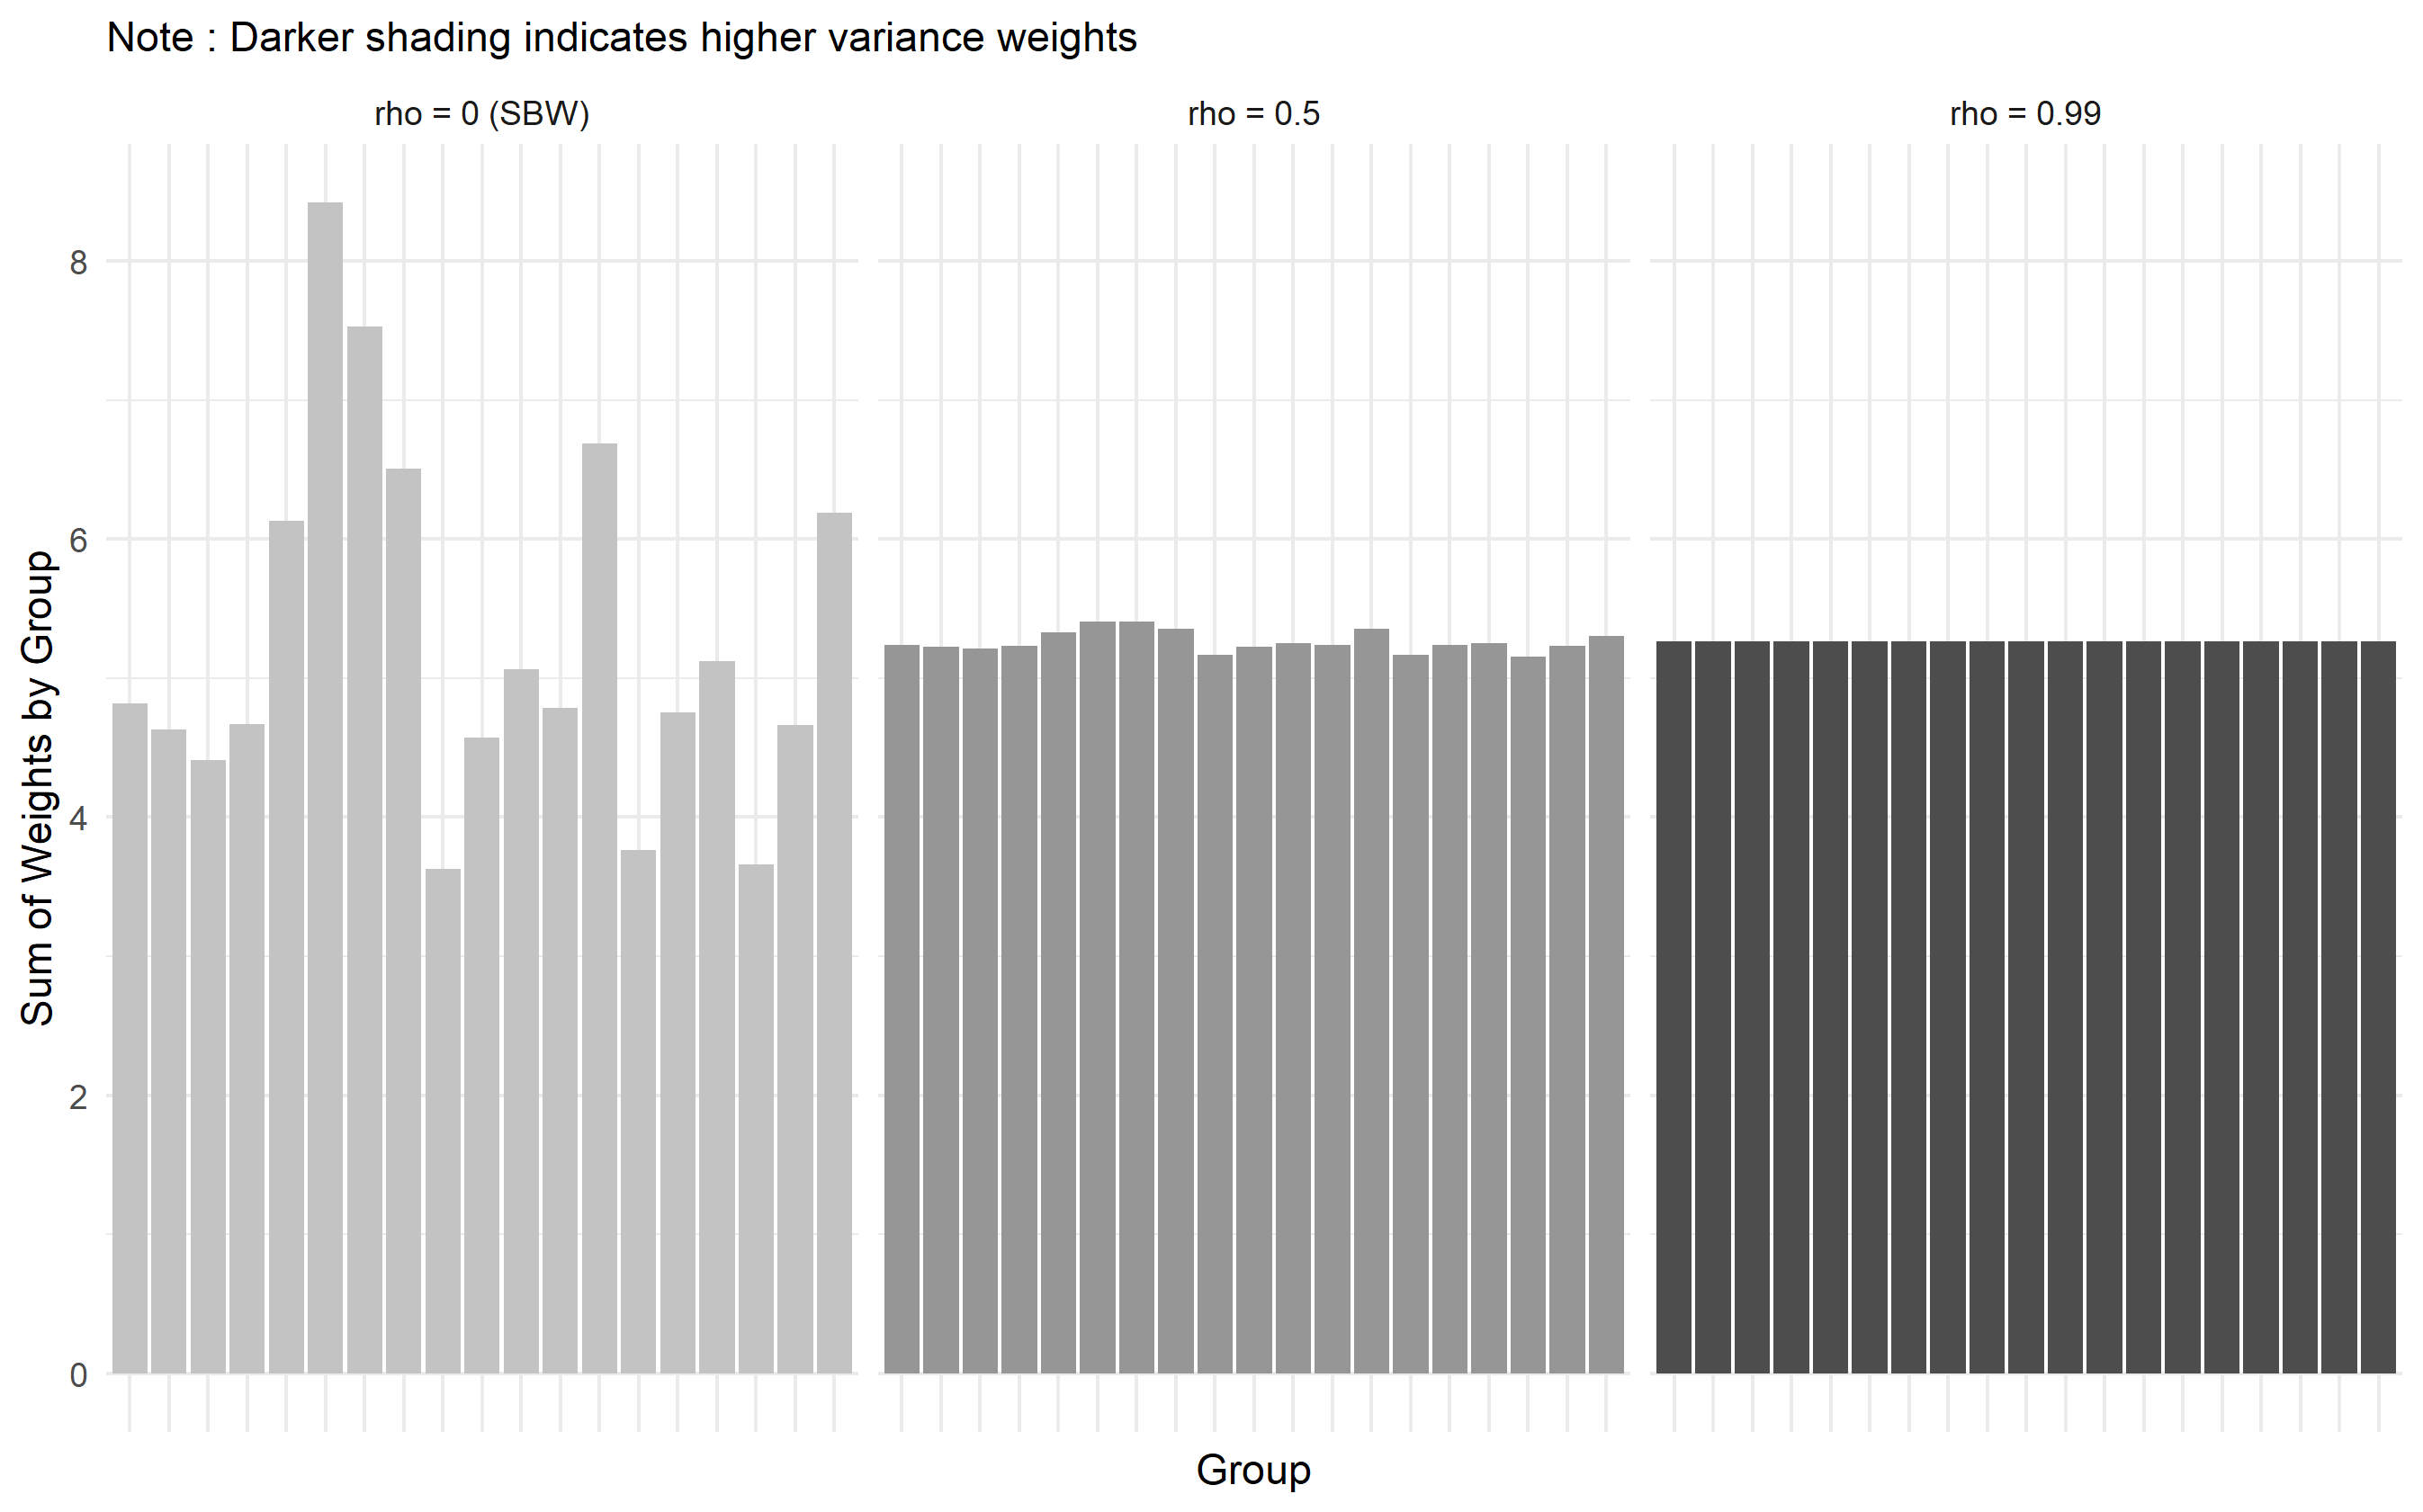
\includegraphics[scale=0.5]{01_Plots/proofofconcept.png}
    \caption{Comparison of SBW and H-SBW: within group sum of weights}
    \label{oatepref}
\end{center}
\end{figure}

The particular covariance structure we assume is identical to the one proposed by \cite{kloek1981ols}. In Appendix A, we show that this objective produces the minimum variance estimator under the constraint set for this correlation structure. We note that theoretically we could incorporate any other assumed covariance structure into this objective, though the number of tuning parameters might change. Broadly speaking, we can think of H-SBW being to SBW what generalized least squares (GLS) is to ordinary least squares (OLS): both SBW and OLS can produce unbiased estimates of model parameters; however, H-SBW and GLS can improve the efficiency of our estimates under different assumed correlation structures of the outcome errors.

\subsubsection{Measurement error}

A second departure in our estimation procedure comes in our balance constraints: rather than balancing on the observed covariate values $W_{sc}$, we instead balance on the imputed covariate estimates $\hat{\eta}_1(W_{sc})$ (we refer to these as the ``adjusted covariates''). This procedure attempts to correct for the estimation error in these CPUMA-level covariates that may bias our estimate of $\psi^1$. In Appendix A, we consider the super-population target $\psi^{1, sp} = \mathbb{E}\{Y^1 \mid A = 0\}$ and show that under the classical errors-in-variables model, the bias for the SBW estimator that balances on the observed covariates $W$ and sets $\delta = 0$ is equivalent to the bias of a linear combination of coefficient estimates from the OLS-based regression estimator. Specifically, the bias for either estimator is:

\begin{equation}
\mathbb{E}\{\hat{\psi}^{1} - \psi^{1, sp}\} = (\upsilon_0 - \upsilon_1)^T(\kappa - I_d)\beta_1
\end{equation}

The intuition for this result is as follows: exact balancing weights implicitly estimate $\beta_1$ on a subset of the data where we have sufficient covariate overlap. We can therefore think of SBW as returning a solution to some weighted-least squares problem. Assuming that the outcome model holds across all of the data, WLS and OLS are estimating the same $\beta_1$; therefore, the bias that effects the least squares solution will have the same effect on the WLS, and therefore SBW, solution. In Appendix A, Proposition 2, we show that if we had access to $\eta_1$, we can obtain an unbiased estimate of $\psi^{1, sp}$ by reweighting $\eta_1(W_{sc})$.\footnote{For the finite-sample parameter we're targeting, this estimator will have finite-sample bias conditional on $W$ and viewing $X$ as fixed.} Of course, in practice we do not know $\eta_1$ but must instead estimate it using auxillary data. In Appendix A, Proposition 3, we show that we can obtain a consistent of $\psi^{1, sp}$ when balancing on an estimate of $\eta_1$ using auxillary data. 

The key in our application is therefore to estimate $\eta_a$: at a high-level, we use the ACS micro-data replicate survey weights to estimate the covariance matrix of CPUMA sampling-variability $\Sigma_{vv, sc}$. Using our observed data to estimate $\Sigma_{WW \mid A = a}$ and $\bar{W}$, we combine these estimates to generate an estimate of $\eta_a$. This is an old technique that comes from the regression-calibration literature (see, e.g., \cite{gleser1992importance}). We also consider an adjustment procedure that further accounts for the differential measurement error due to the highly variable sample sizes used to calculate each covariate. Specifically, letting $s_{sc}$ be the $q$ dimensional vector of (known) sample sizes, we consider the model $\sqrt{s}_{sc} \cdot v_{sc} \stackrel{iid}\sim MNV(0, \Sigma_{vv \mid A = a})$. By pooling the individual $\hat{\Sigma}_{vv, sc}$ using $s_{sc}$, we can then generate a modeled estimate $\hat{\Sigma}^m_{vv, sc}$ that uses the full efficiency of the data (which we model separately by treatment status). We then use these estimates generate a CPUMA-specific $\hat{\kappa}_{sc}$. This procedure allows our adjustment to differentially adjust covariate values depending on the sample-sizes involved in the adjustment procedure. Further details about these procedures are available in Appendix B.

This is the first application we are aware of to use regression calibration in the context of balancing weights to address the problem of measurement error. We emphasize two critical assumptions for using this procedure in our context: (1) the outcome model is linear in the true covariates; and (2) the measurement error in the outcome is uncorrelated with the measurement error in the covariates. The first assumption is strong, though often used in practice. The second assumption is reasonable, because our outcomes are estimated from a different cross-section than our covariates. 

\subsubsection{Bias-correction for imbalances}

Because we are unable to reduce the balance constraints to our preferred level without generating very extreme weights, following the recent literature on synthetic controls, we test the sensitivity of our results to these imbalances by using ridge-regression augmented weights \cite{ben2018augmented}. Letting $\matr{\hat{X}}_1$ be the matrix of adjusted covariates, and $\gamma^{hsbw}$ be our H-SBW weights, we consider the regression-augmented weights:

\begin{equation}
\gamma^{aug} = \gamma^{hsbw} + (\matr{\hat{X}}_1^T\gamma^{hsbw} - \bar{\matr{W}}_0)^T(\matr{\hat{X}}_1^T\Omega^{-1}\matr{\hat{X}}_1 + \lambda I_q)^{-1}\matr{\hat{X}}_1^T\Omega^{-1}
\end{equation}

where $\Omega$ is a block diagonal matrix with diagonal entries equal to one and the within-group off diagonals equal to $\rho$. We choose $\lambda$ so that the remaining imbalances all fall within 0.5 percentage points. The cost of this procedure is that we must extrapolate off the support of the data, and therefore rely more heavily on our outcome modeling assumptions. We refer to \cite{ben2018augmented} for more details about this procedure. In our results we consider estimators using SBW ($\rho = 0$), H-SBW ($\rho = 0.2$), and ridge-augmented versions of SBW and H-SBW that we call BC-SBW and BC-HSBW. 

\subsection{Model validation}

While we argue that we cannot use pre-treatment outcomes to conduct variable selection or to learn about the relative importance of covariates, we argue that we can use validation period data to compare the performance of different models for fixed covariates and selected levels of imbalance $\delta$. More generally, the best model of $\mu_{0, t}$ $(t = 1,..., T-1)$ is not necessarily the best model, or even a good model, of $\mu_{1, T}$ and vice versa. We invoke additional assumptions to claim the latter: that a good model of $\mu_{1, T}$ is a good model of $\mu_{0, t}$.

First, we again assume the models for $\mu_{a, t}$ are linear in the covariates $\matr{X}$ for all time periods $t$. This is a stronger assumption than required to identify the ETC, which is only that $Y^1_T \perp A \mid X$. Second, we assume that $\matr{X}$ at worst contains some irrelevant covariates $V$ for the model $\mu_{0, t}$. Third, assume that there is a feasible $\delta$ such that all covariate imbalances are small. Under these assumptions, it is easy to see that the best model of $\psi^1$ for time $T$ should also be a good model for $n_t^{-1}\sum_{s,c: A_{sc} = 1}Y_{sct}^0$ for $t = T-l,...,T$ when trained on data from $t = 1, ..., T-l-1$. Even so, we again note that the best model of $\mu_{0, t}$ is not necessarily the best model of $\mu_{1, t}$.

We therefore rerun our procedures on pre-treatment data to compare the performance of our models for a fixed level of imbalances $\delta$. In particular, we train our model on 2009-2011 data to predict 2012 outcomes, and 2010-2012 data to predict 2013 outcomes, and present the errors. We limit to one-year prediction error since our estimand is only one-year forward. We then examine the performance of the H-SBW versus SBW estimators, which only vary with respect to the tuning parameter $\rho$, the bias-corrected versions, and the covariate adjustment procedure used. 

If our outcome models are correct, we expect that the only differences will be due to the covariate adjustment procedure: the adjustment that allows us to best reduce the true (unobserved) covariate imbalances should perform best. This procedure can therefore inform us which covariate adjustment is optimal. We can also examine the tradeoffs from extrapolation versus imbalances: if the outcome model is at best an approximation, we may find that extrapolation does not reduce the bias of the procedure. Finally, we expect that H-SBW versus SBW should have similar performance. However, in Appendix A, we do show that for fixed (unobserved) $X$, the estimator has finite sample bias that reduces with the square of the weights, suggesting the SBW may have less bias than H-SBW; however, we believe will that H-SBW should have less variability. It is unclear how this tradeoff will play out, especially given that we have only two years of pre-treatment data to conduct this test on.

\subsection{Inference}

We consider $W$ to be fixed (and $X$ as fixed unknown parameters), and we consider inference over repeated samples from some super-population of CPUMAs with a state-level dependency structure.\footnote{Alternatively, viewing the potential outcomes as fixed and treatment assignment as random, we could consider inference over the randomization distribution of treatment at the state-level.} While placebo tests are frequently used in the synthetic controls literature for inference, we view these as qualitative statistical tests (see, e.g., \cite{arkhangelsky2019synthetic}) and instead use the leave-one-state-out jackknife to estimate the variance of $\hat{\psi}^1$ (\cite{cameron2015practitioner}). Specifically, we exclude each state and re-calculate the weights holding our targeted mean fixed at $\bar{W}_0$.\footnote{When our preferred initial choice of $\delta$ does not converge, we gradually reduce the constraints until it does.} We compute this estimator in two ways: first, we condition on our covariate adjustment $\hat{\eta}_1$. This is our preferred estimator; however, it does not account for the randomness in $\hat{eta}_1$. We therefore also conduct a second procedure where we re-estimate $\hat{\eta}_1$ for each state omitted in the jackknife procedure and provide these results in the Appendix.

To estimate $Var(\hat{\psi}^0 \mid X, W)$ we use an auxillary regression model and use the CR-2 standard error adjustment (using the ``clubSandwich'' package in R) to estimate the variance of the linear combination $\bar{W}_0^T\hat{\beta}_0$. We can estimate this quantity using the original (unadjusted) data given that $\mathbb{E}\{\bar{W}_0^T\hat{\beta}_0\} = \psi^0$ (since the regression line runs through the point $(\bar{W}_0, \bar{J}_0)$, which are unbiased estimates of $(\bar{X}_0, \bar{Y}_0)$). Our total estimate $\hat{Var}(\hat{\psi})$ is simply the sum of these two variance estimates. We use the standard normal quantiles to generate confidence intervals. 


\section{Results}
This section presents our results. The first sub-section contains summary statistics regarding the variability of six key covariates pre- and post- adjustment to address measurement error. The second sub-section contains covariate balance diagnostics. The third sub-section contains our primary ETC results, presenting our estimates of the treatment effect and a series of sensitivity analyses. The final sub-section contains our analysis of covariate importance and investigation into treatment effect heterogeneity.

\subsection{Covariate adjustment}

We first examine the effects of our covariate adjustments on the variance of our pre-treatment outcomes and pre-treatment unemployment rates among the expansion states. We most heavily prioritize balancing these covariates, but they are also among the least precisely estimated (all of our other covariates average over three years of data, rather than just one). Table~\ref{tab:adjust1} displays the variance of each covariate on the unadjusted and adjusted datasets. We see that both the homogeneous and heterogeneous adjustment procedures reduce the variability in the data by comparable amounts. Intuitively, the adjustment to address measurement error reduces the likelihood that our balancing weights will over-fit to noise in the data. These results are consistent across most of our other covariates.

\begin{table}[ht]
\caption{Sample variance on unadjusted and adjusted datasets, expansion states}
\label{tab:adjust1}
\begin{tabular}{lrrr}
  \hline
Variable & No adjustment & Heterogeneous & Homogeneous \\ 
  \hline
Uninsured Pct 2011 & 8.35 & 8.04 & 8.05 \\ 
  Uninsured Pct 2012 & 8.20 & 7.89 & 7.90 \\ 
  Uninsured Pct 2013 & 8.09 & 7.78 & 7.79 \\ 
  Unemployed Pct 2011 & 3.66 & 3.25 & 3.27 \\ 
  Unemployed Pct 2012 & 3.72 & 3.38 & 3.38 \\ 
  Unemployed Pct 2013 & 3.20 & 2.88 & 2.87 \\ 
   \hline
\end{tabular}
\end{table}

\subsection{Covariate balance}

Figure~\ref{fig:loveplotc1} displays the reduction of imbalances using our H-SBW weights. This plot only displays covariates with greater than one percentage point difference between the targeted mean in the expansion region and the mean values in the non-expansion region prior to weighting, and the reweighted treatment values use our preferred covariate adjustment $\hat{\eta}_1(W_{sc})$. Before applying our weights, we see that there are substantial imbalances in the Republican governance indicators, as well as pre-treatment uninsurance and unemployment rates. Our weights reduce these differences; however, some remain, particularly among the Republican governance indicators. A complete balance table is available in Appendix D, Table~\ref{tab:baltab1}. 

\begin{figure}[H]
\begin{center}
    \caption{Balance plot, primary dataset}
    \label{fig:loveplotc1}
    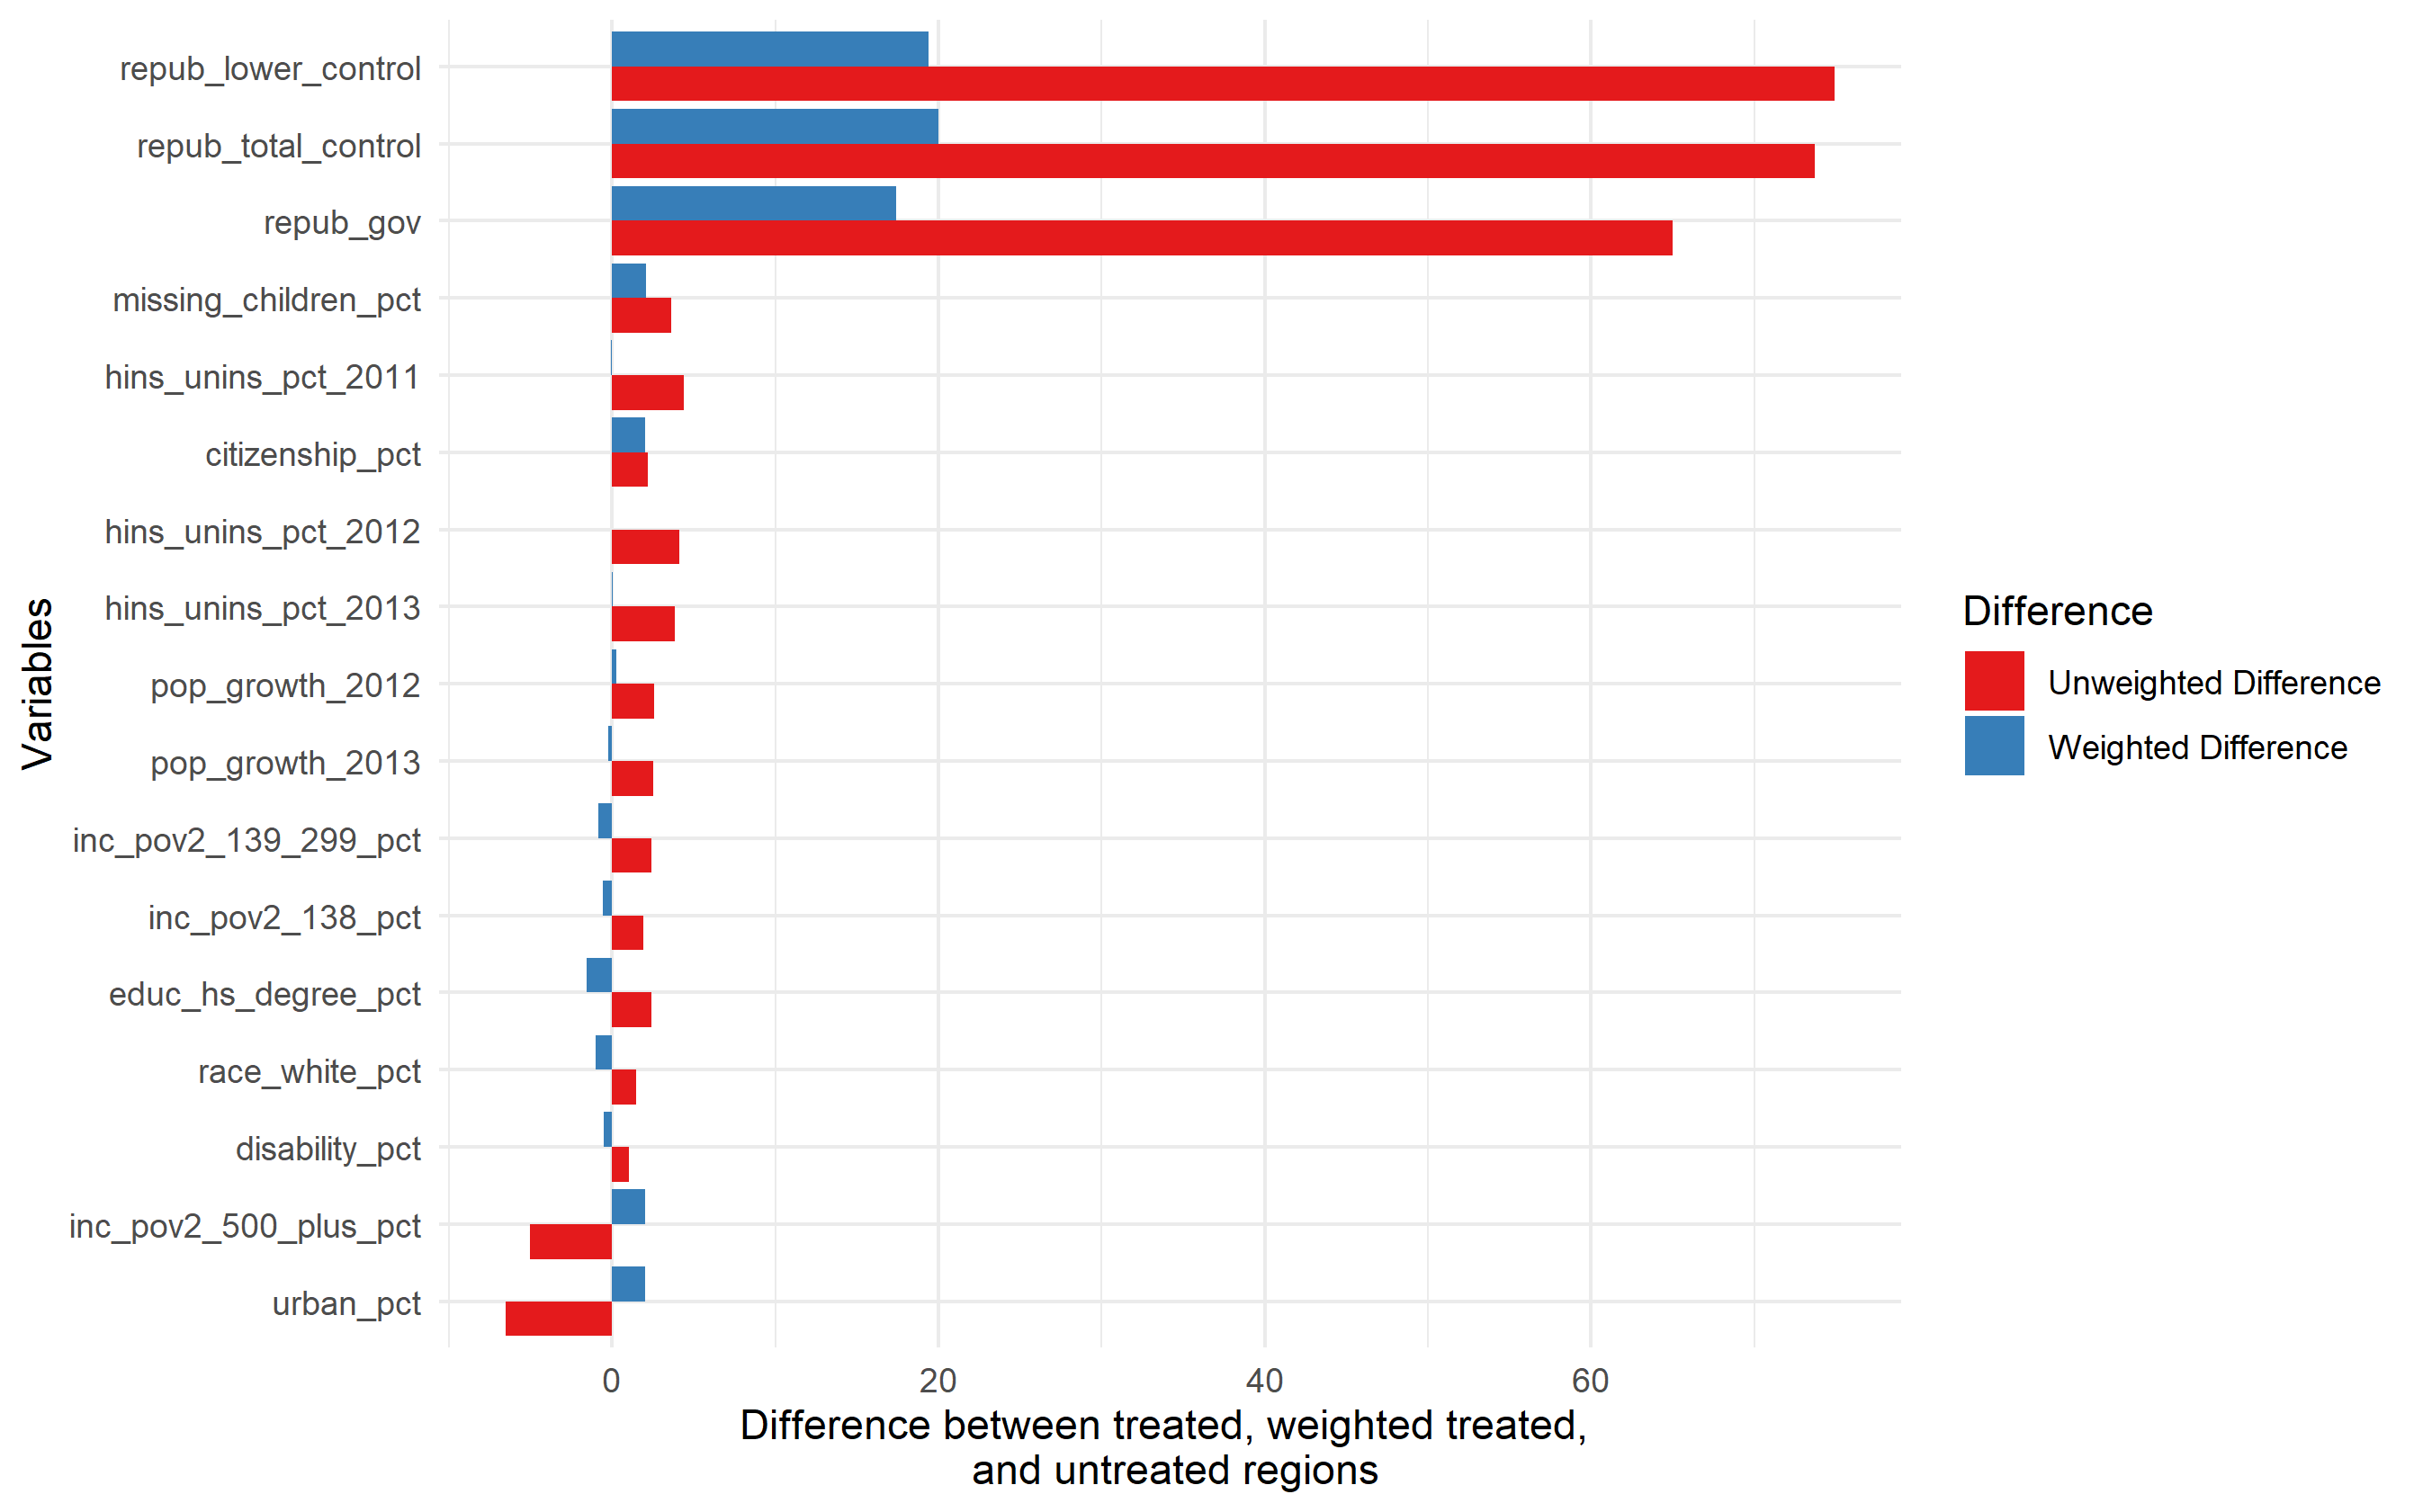
\includegraphics[scale=0.6]{01_Plots/balance-plot-etuc1.png}
\end{center}
\end{figure}

We also compare the H-SBW estimator to the SBW estimates in Figure~\ref{fig:sbwvhsbw1}. We see that H-SBW more evenly distributes the weights across states relative to SBW, particularly by reducing the amount of weight given to CPUMAs in Ohio. 

\begin{figure}[H]
\begin{center}
    \caption{H-SBW versus SBW, weights summed by state, primary dataset}
    \label{fig:sbwvhsbw1}
    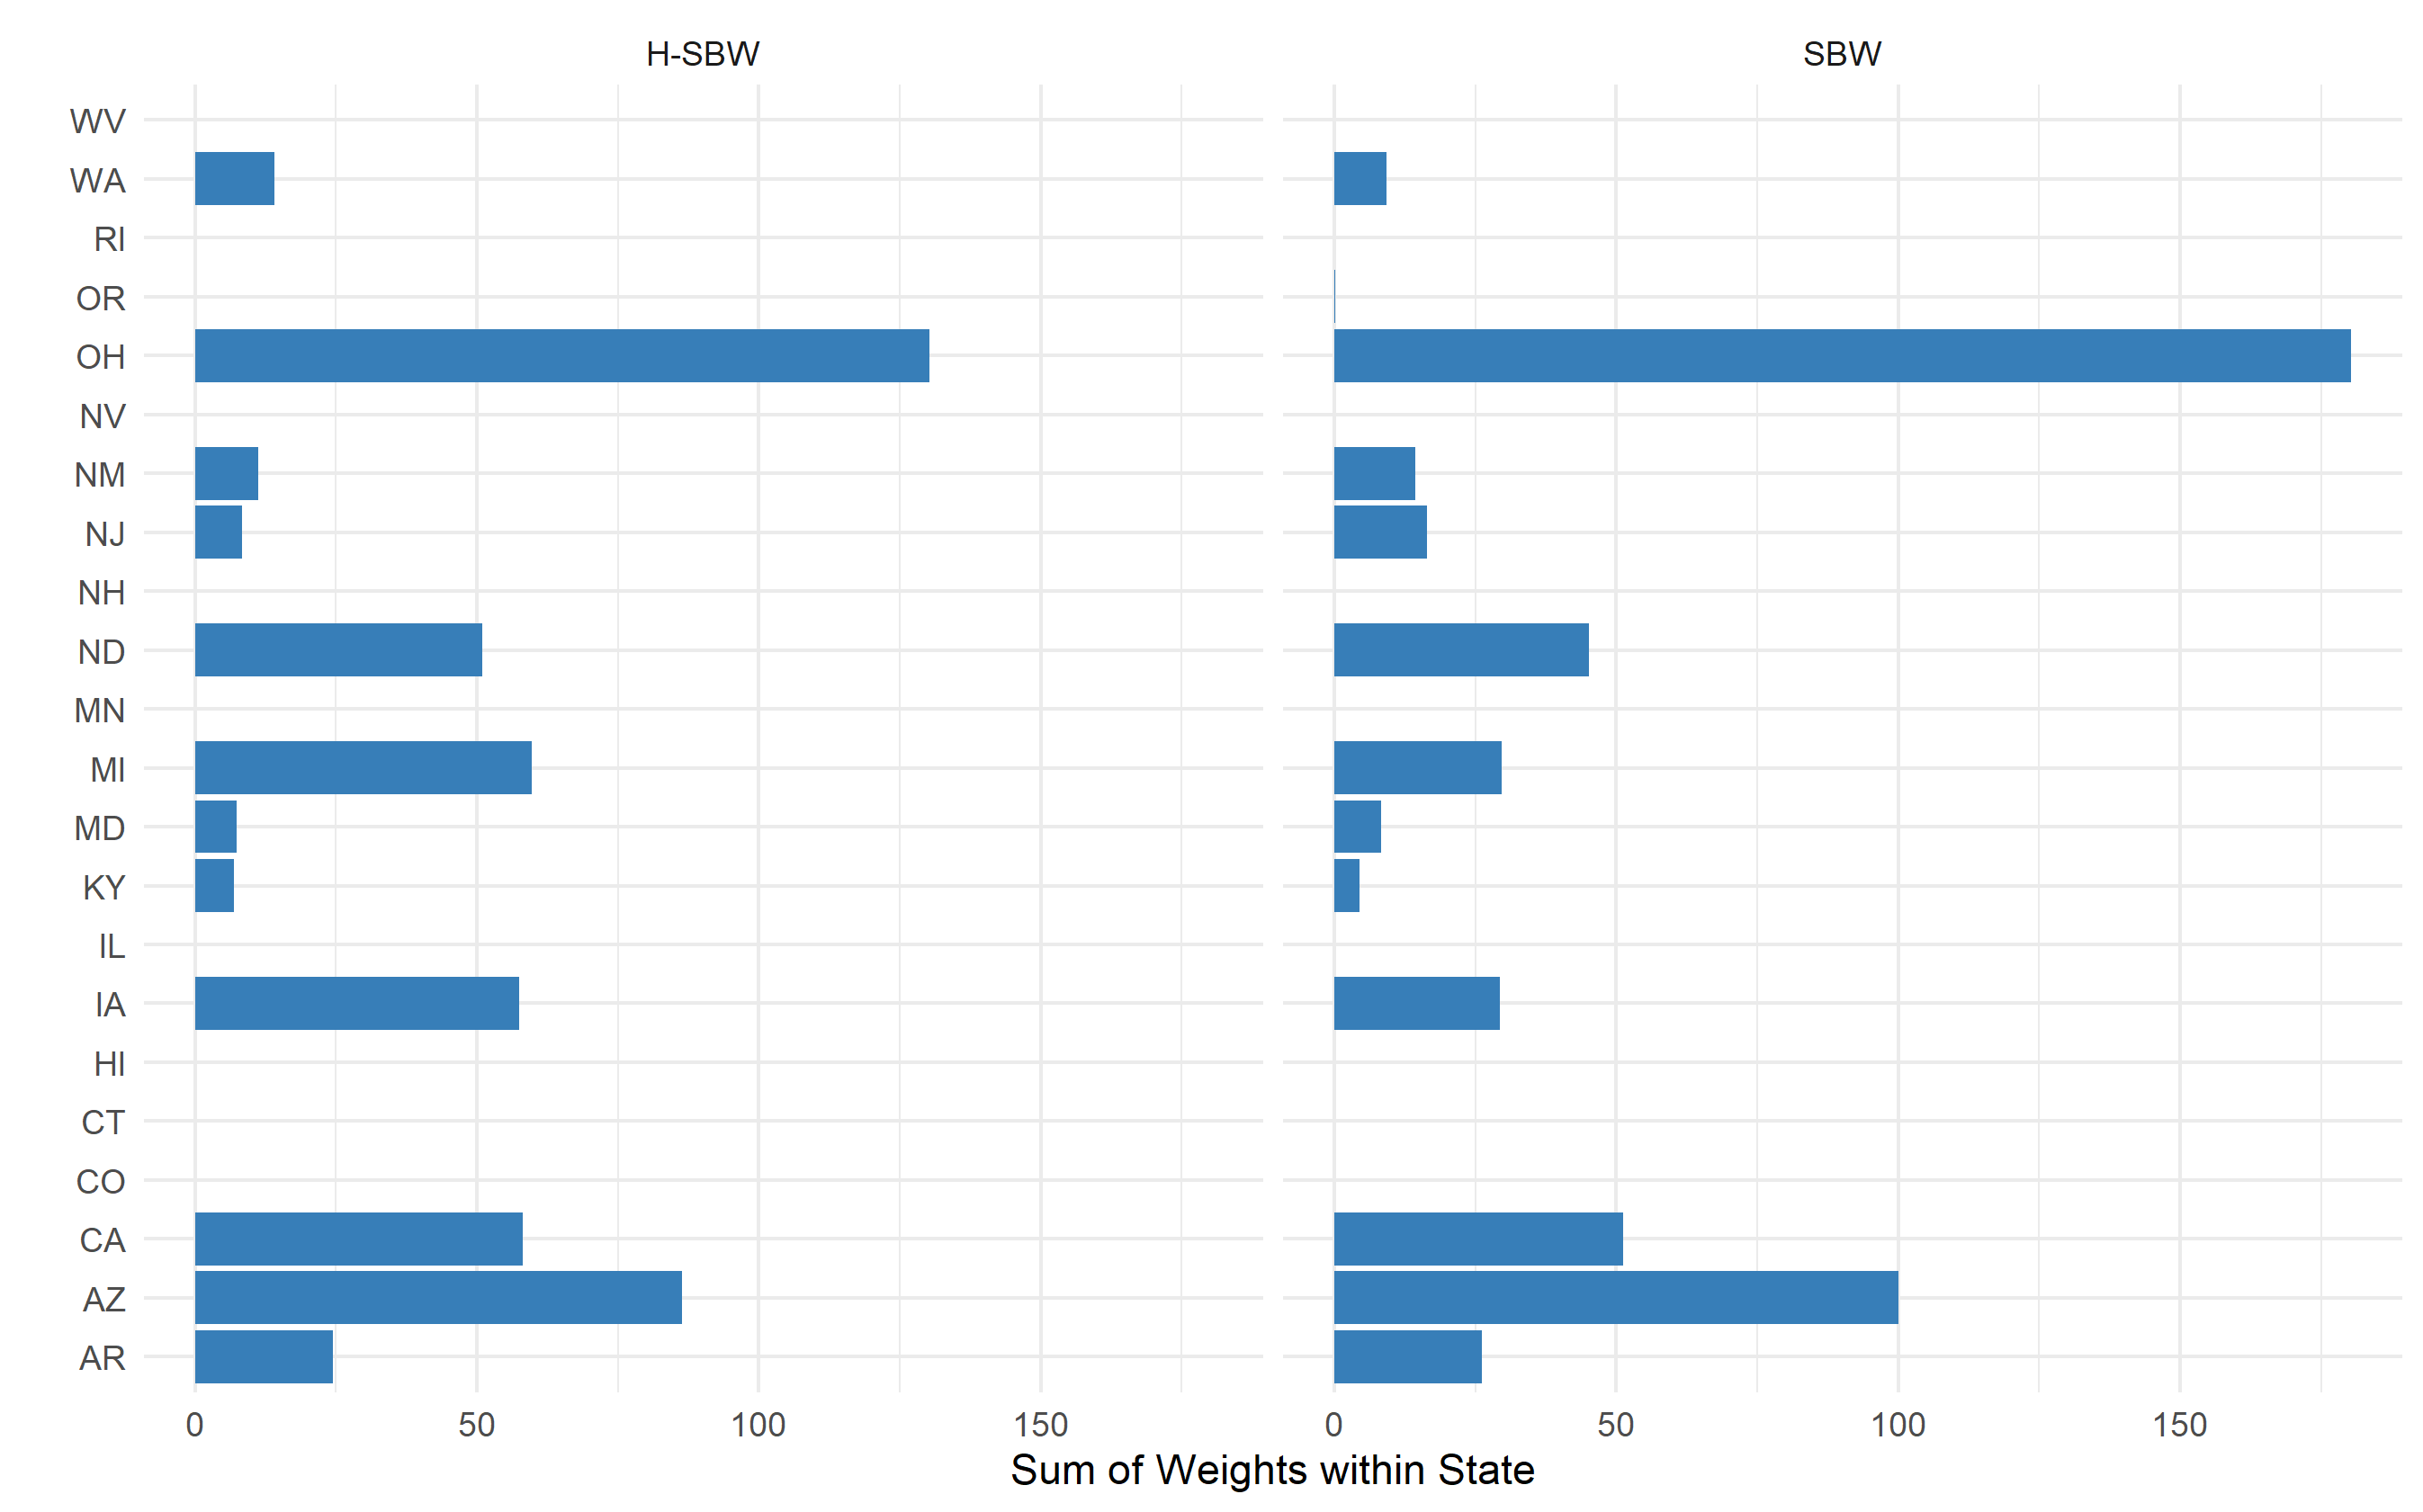
\includegraphics[scale=0.6]{01_Plots/weights-by-state-sbw-hsbw-c1.png}
\end{center}
\end{figure}

We then use ridge-regression augmentation to extrapolate from the data in order to reduce all imbalances within 0.5 percentage points. Figure~\ref{fig:statewghts} shows the total weights summed across states for two estimators: H-SBW and BC-HSBW. This figure sums the negative weights separately from the positive weights to show the extent of the extrapolation. We see that BC-HSBW extrapolates somewhat heavily in order to achieve the desired level of balance, particularly for CPUMAs in California. 

\begin{figure}[H]
\begin{center}
    \caption{H-SBW versus BC-HSBW, weights summed by state, primary dataset}
    \label{fig:statewghts}
    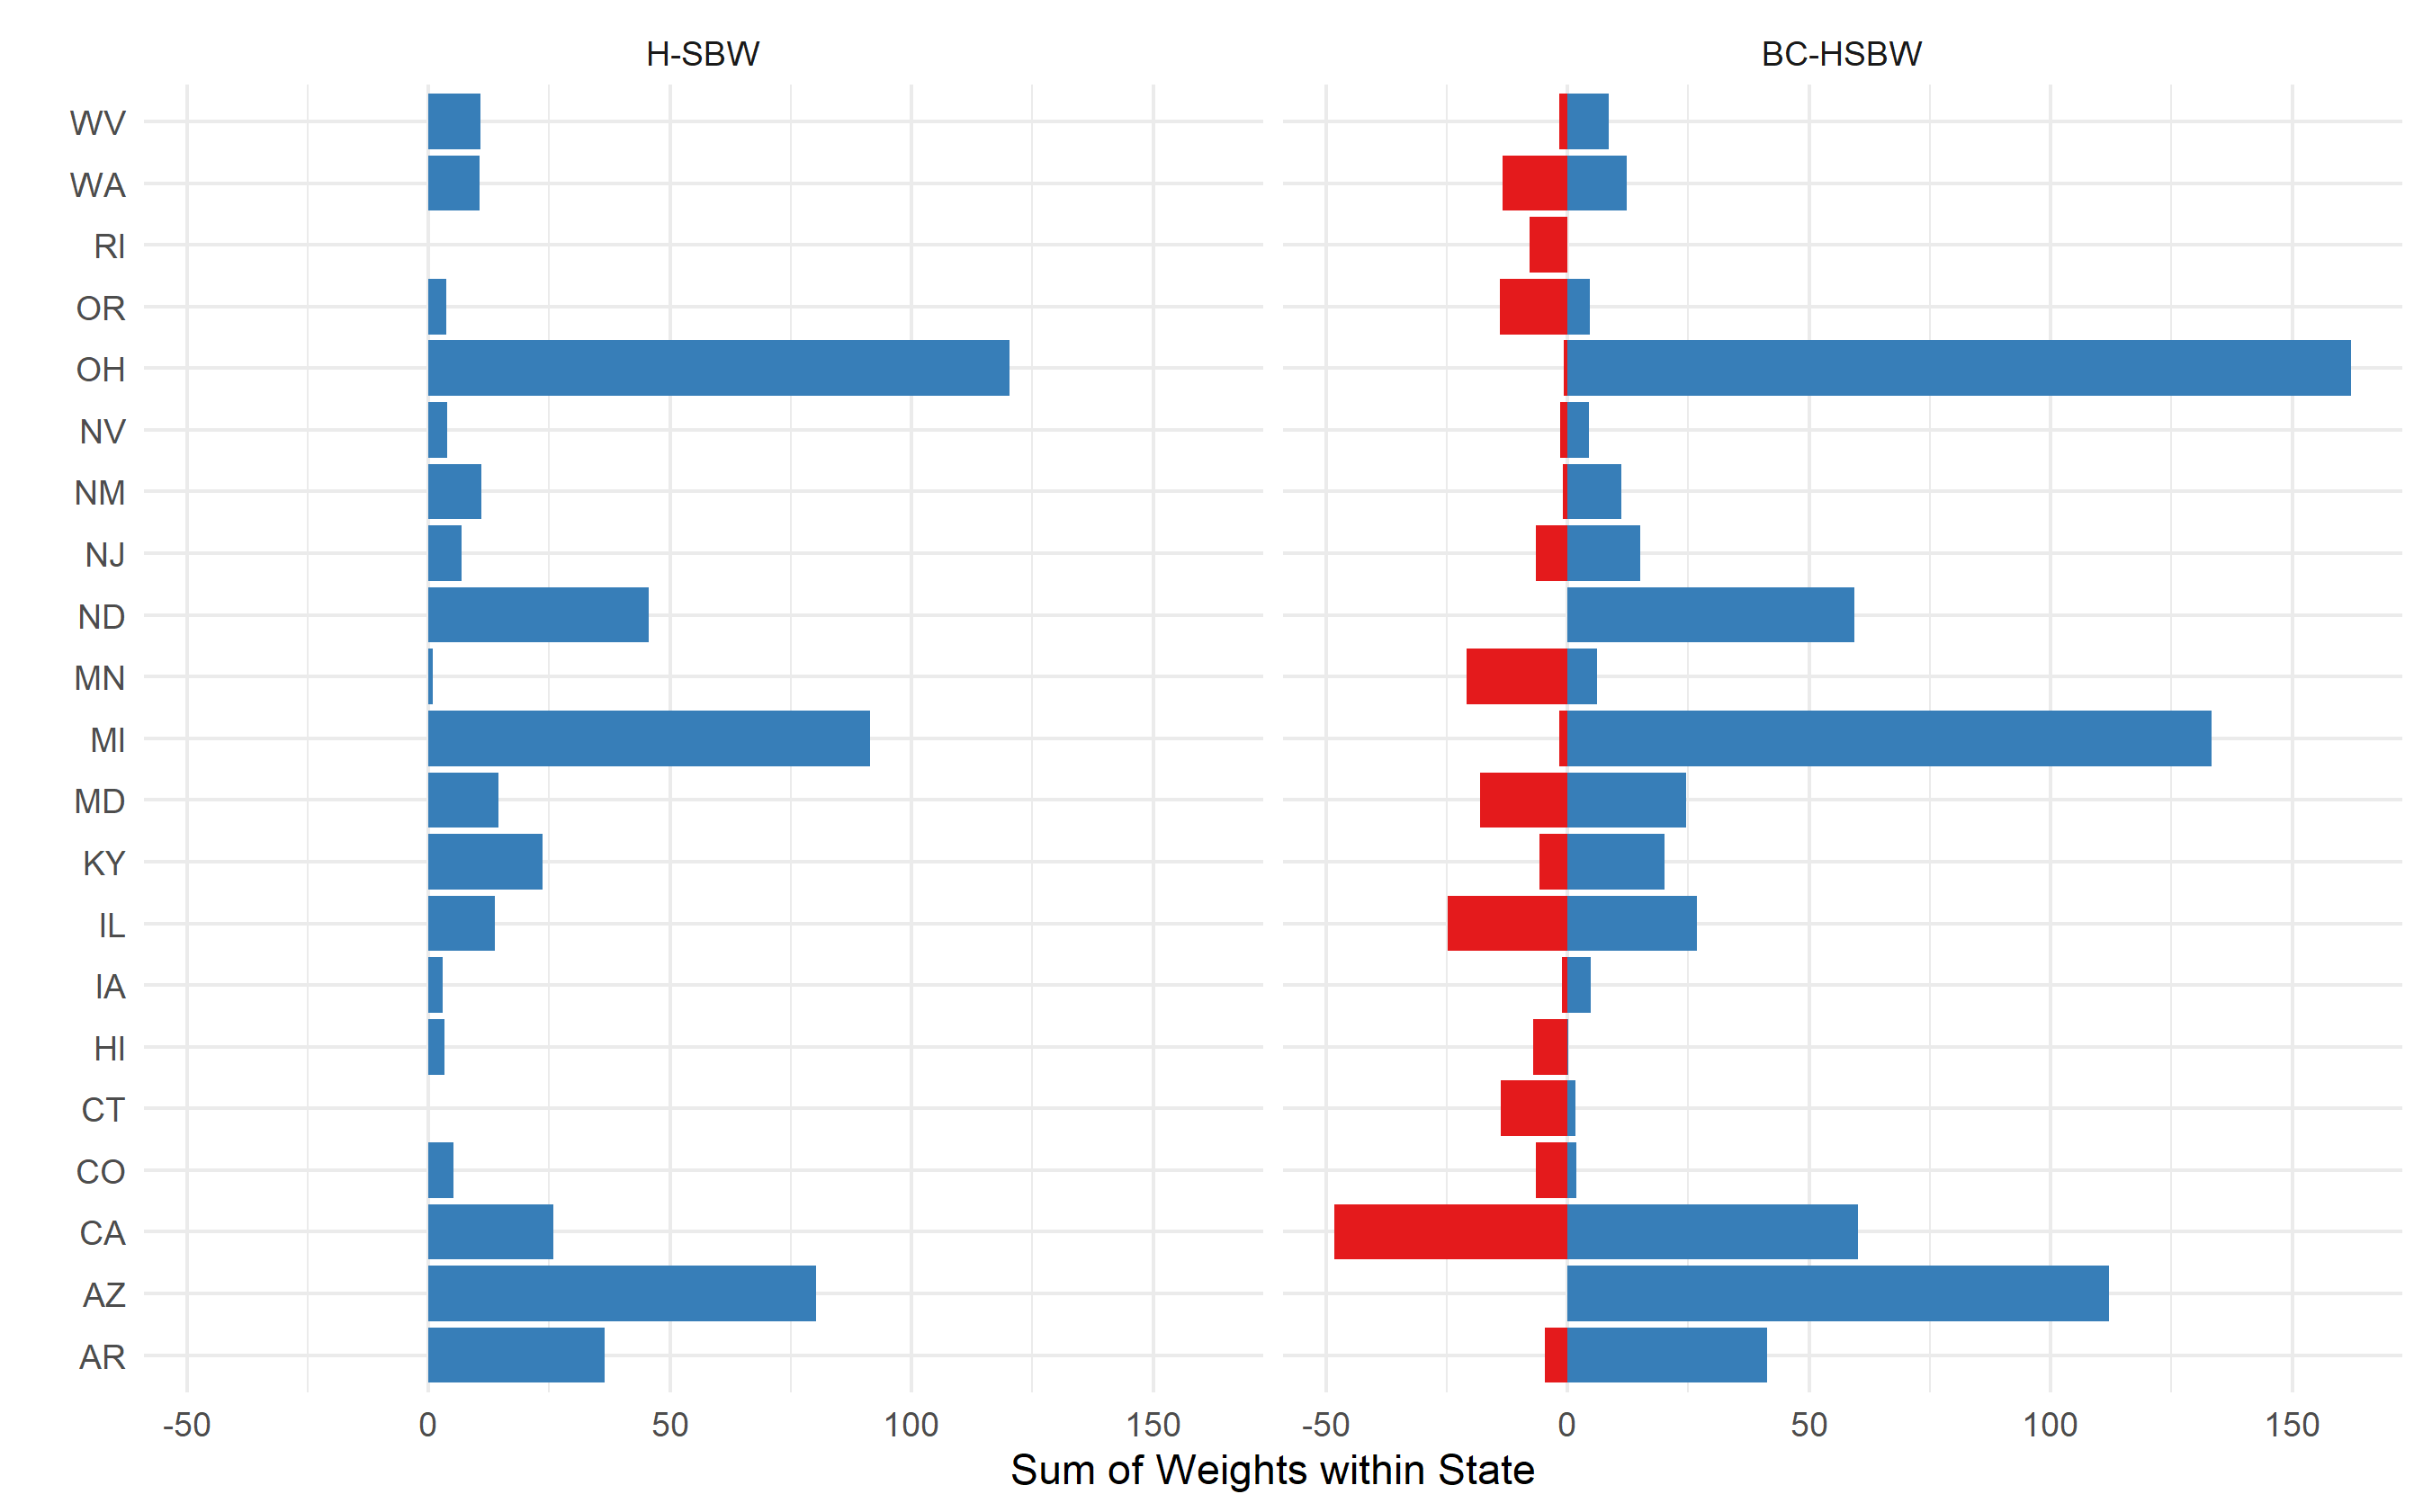
\includegraphics[scale=0.6]{01_Plots/weights-by-state-hsbw-c1.png}
\end{center}
\end{figure}

Finally, we wish to see whether the weights generated using the unadjusted data balance the adjusted covariates. While this balance measure does not reflect the ``true'' imbalances, this comparison does give some indication of whether the unadjusted weights are overfitting to noisy covariate measurements. Table~\ref{tab:balcomp} compares the imbalances among our pre-treatment outcomes and uninsurance rates using H-SBW weights generated on our unadjusted dataset applied to the adjusted (homogeneous) dataset. The ``Unweighted Difference'' column represents the raw difference in means, while the ``Weighted Diff'' column reflects the weighted difference that we calculate on the unadjusted dataset. The ``Homogeneous Diff'' column displays the weighted imbalance when applying the H-SBW weights to the dataset using the homogeneous adjustment, and likewise for ``Heterogeneous Diff.'' We see that the weighted pre-treatment outcomes are approximately one percentage point lower than we desired in the two years prior to treatment using the heterogeneous adjustment, and -0.2 percentage points lower (on average) using the homogeneous adjustment. Given the high degree of correlation between pre-treatment outcomes, we may expect the estimator of $\psi^1$ trained on the unadjusted data to have some downward bias.

\begin{table}[ht]
\caption{Balance comparison: unadjusted weights on adjusted data}
\label{tab:balcomp}
\begin{tabular}{lrrrr}
  \hline
Variables & Unweighted Diff & Weighted Diff (none) & Homogeneous Diff & Heterogeneous Diff\\ 
  \hline
Uninsured Pct 2011 & -3.09 & -0.05 & -0.11 & 0.92 \\ 
  Uninsured Pct 2012 & -2.99 & -0.05 & -0.21 & -1.06 \\ 
  Uninsured Pct 2013 & -3.00 & -0.05 & -0.38 & -0.93 
   \hline
\end{tabular}
\end{table}

\subsubsection{Model validation}

We compare the performance of our models by repeating the covariate adjustments and calculating our procedure on 2009-2011 ACS data to predict 2012 outcomes, and similarly for 2010-2012 data to predict 2013 outcomes for the treated states. Table~\ref{tab:pretxpred} see that the estimators trained on the covariate adjusted data have substantially better performance than the unadjusted data. Moreover, the estimators trained on the homogeneous adjustment seem to do slightly better than the ones that model the heterogeneity; we therefore prioritize presenting results on the homogeneous adjustment. We also find that SBW tends to have slightly lower bias than H-SBW. This is consistent with our theoretic results in Appendix A, which show that the bias should decrease with the square of the weights for fixed $X$. Despite these results, H-SBW may have lower variance (and possibly MSE) given our assumed dependencies in the model errors. We therefore do not use these results to prefer H-SBW or SBW. Finally, we see that the bias corrected estimators tend to perform worse in this application. This indicates that the extrapolation bias outweighs the cost of the covariate imbalances. While this does not necessarily imply this should hold for the model of $Y^1_T$, it does caution against these results. We see this as a function of our models as best reflecting an approximation: we expect in general that assuming the linear outcome models approximately holds on the support of the data where we have sufficient covariate overlap, but we these models may lead us astray when our weights extrapolate excessively from the data. The worst performing estimators are the bias-corrected estimators trained on the unadjusted data.

\begin{table}[ht]
\caption{Estimator pre-treatment outcome prediction error}
\label{tab:pretxpred}
\begin{tabular}{llrrr}
  \hline
Sigma estimate & Estimator & 2012 error & 2013 error & RMSE \\ 
  \hline
Homogeneous & SBW & -0.18 & -0.22 & 0.20 \\ 
  Homogeneous & H-SBW & -0.24 & -0.21 & 0.23 \\ 
  Heterogeneous & SBW & -0.25 & -0.30 & 0.27 \\ 
  Heterogeneous & H-SBW & -0.32 & -0.39 & 0.36 \\ 
  Homogeneous & BC-SBW & -0.42 & -0.35 & 0.39 \\ 
  Heterogeneous & BC-SBW & -0.45 & -0.39 & 0.42 \\ 
  None & SBW & -0.50 & -0.61 & 0.56 \\ 
  None & H-SBW & -0.52 & -0.61 & 0.57 \\ 
  Homogeneous & BC-HSBW & -0.53 & -0.62 & 0.58 \\ 
  Heterogeneous & BC-HSBW & -0.53 & -0.72 & 0.63 \\ 
  None & BC-SBW & -0.82 & -0.93 & 0.88 \\ 
  None & BC-HSBW & -0.93 & -0.99 & 0.96 \\ 
   \hline
\end{tabular}
\end{table}

Finally, we find a consistent negative bias across all of our estimators: that is, all of our models tend to under-predict the true uninsurance rate among the non-expansion states the subsequent year. If we believe that the sign of this bias will also afflict our estimates of $\bar{Y}^1$, then we should expect our treatment effect estimates to have downward bias (which would bias our estimates away from zero). That is, the true treatment effect may be smaller (closer to zero) in absolute magnitude than the estimated treatment effect. If we believe the bias will also have comparable magnitude, these results suggests that the true treatment effect will be approximately 0.2 to 0.5 percentage points closer to zero than the estimated effect.

\subsection{Primary Results}

Using H-SBW we estimate an effect of -2.33 (-3.49, -1.16) percentage points. The SBW results are almost identical with -2.35 (-3.65, -1.06) percentage points. Compared to the unadjusted data we see very similar estimates at -2.34 (-2.85, -1.82) percentage points for H-SBW and -2.39 (-2.95, -1.83) percentage points for SBW. We see that H-SBW reduces the confidence intervals relative to SBW. We also observe that using the adjusted covariate set appears to increases the width of the estimated confidence intervals. This increase in variability is expected because the adjustment procedure generally reduces the variability in the data, as we saw in Table~\ref{tab:adjust1}, thereby requiring that the balancing weights also increase in variability to achieve the desired level of balance. Importantly, this variance estimate conditions on the covariate adjustment, and does not take into account the randomness in this procedure, and may therefore understate the true uncertainty. When we recalculate the entire adjustment procedure, we find that the confidence intervals are of a comparable magnitude. The results are available in Appendix E.

When we add the bias-correction, the absolute magnitude of the point estimate decreases: we estimate -2.05 (-3.32, -0.79) percentage points for BC-HSBW and -2.00 (-2.98, -1.01) percentage points for BC-SBW. In contrast to the H-SBW and SBW estimators, we see that the confidence interval for BC-SBW is narrower than for BC-HSBW. Figure~\ref{fig:estimators} presents all of our estimates. All adjusted estimates were closer to zero than the unadjusted estimates, though the point estimates from the SBW and H-SBW were estimators were virtually identical. The heterogeneous adjustments were all closer to zero than the unadjusted estimates; results are available in Appendix E.

\begin{figure}[H]
\begin{center}
    \caption{Primary point estimates and confidence intervals}
    \label{fig:estimators}
    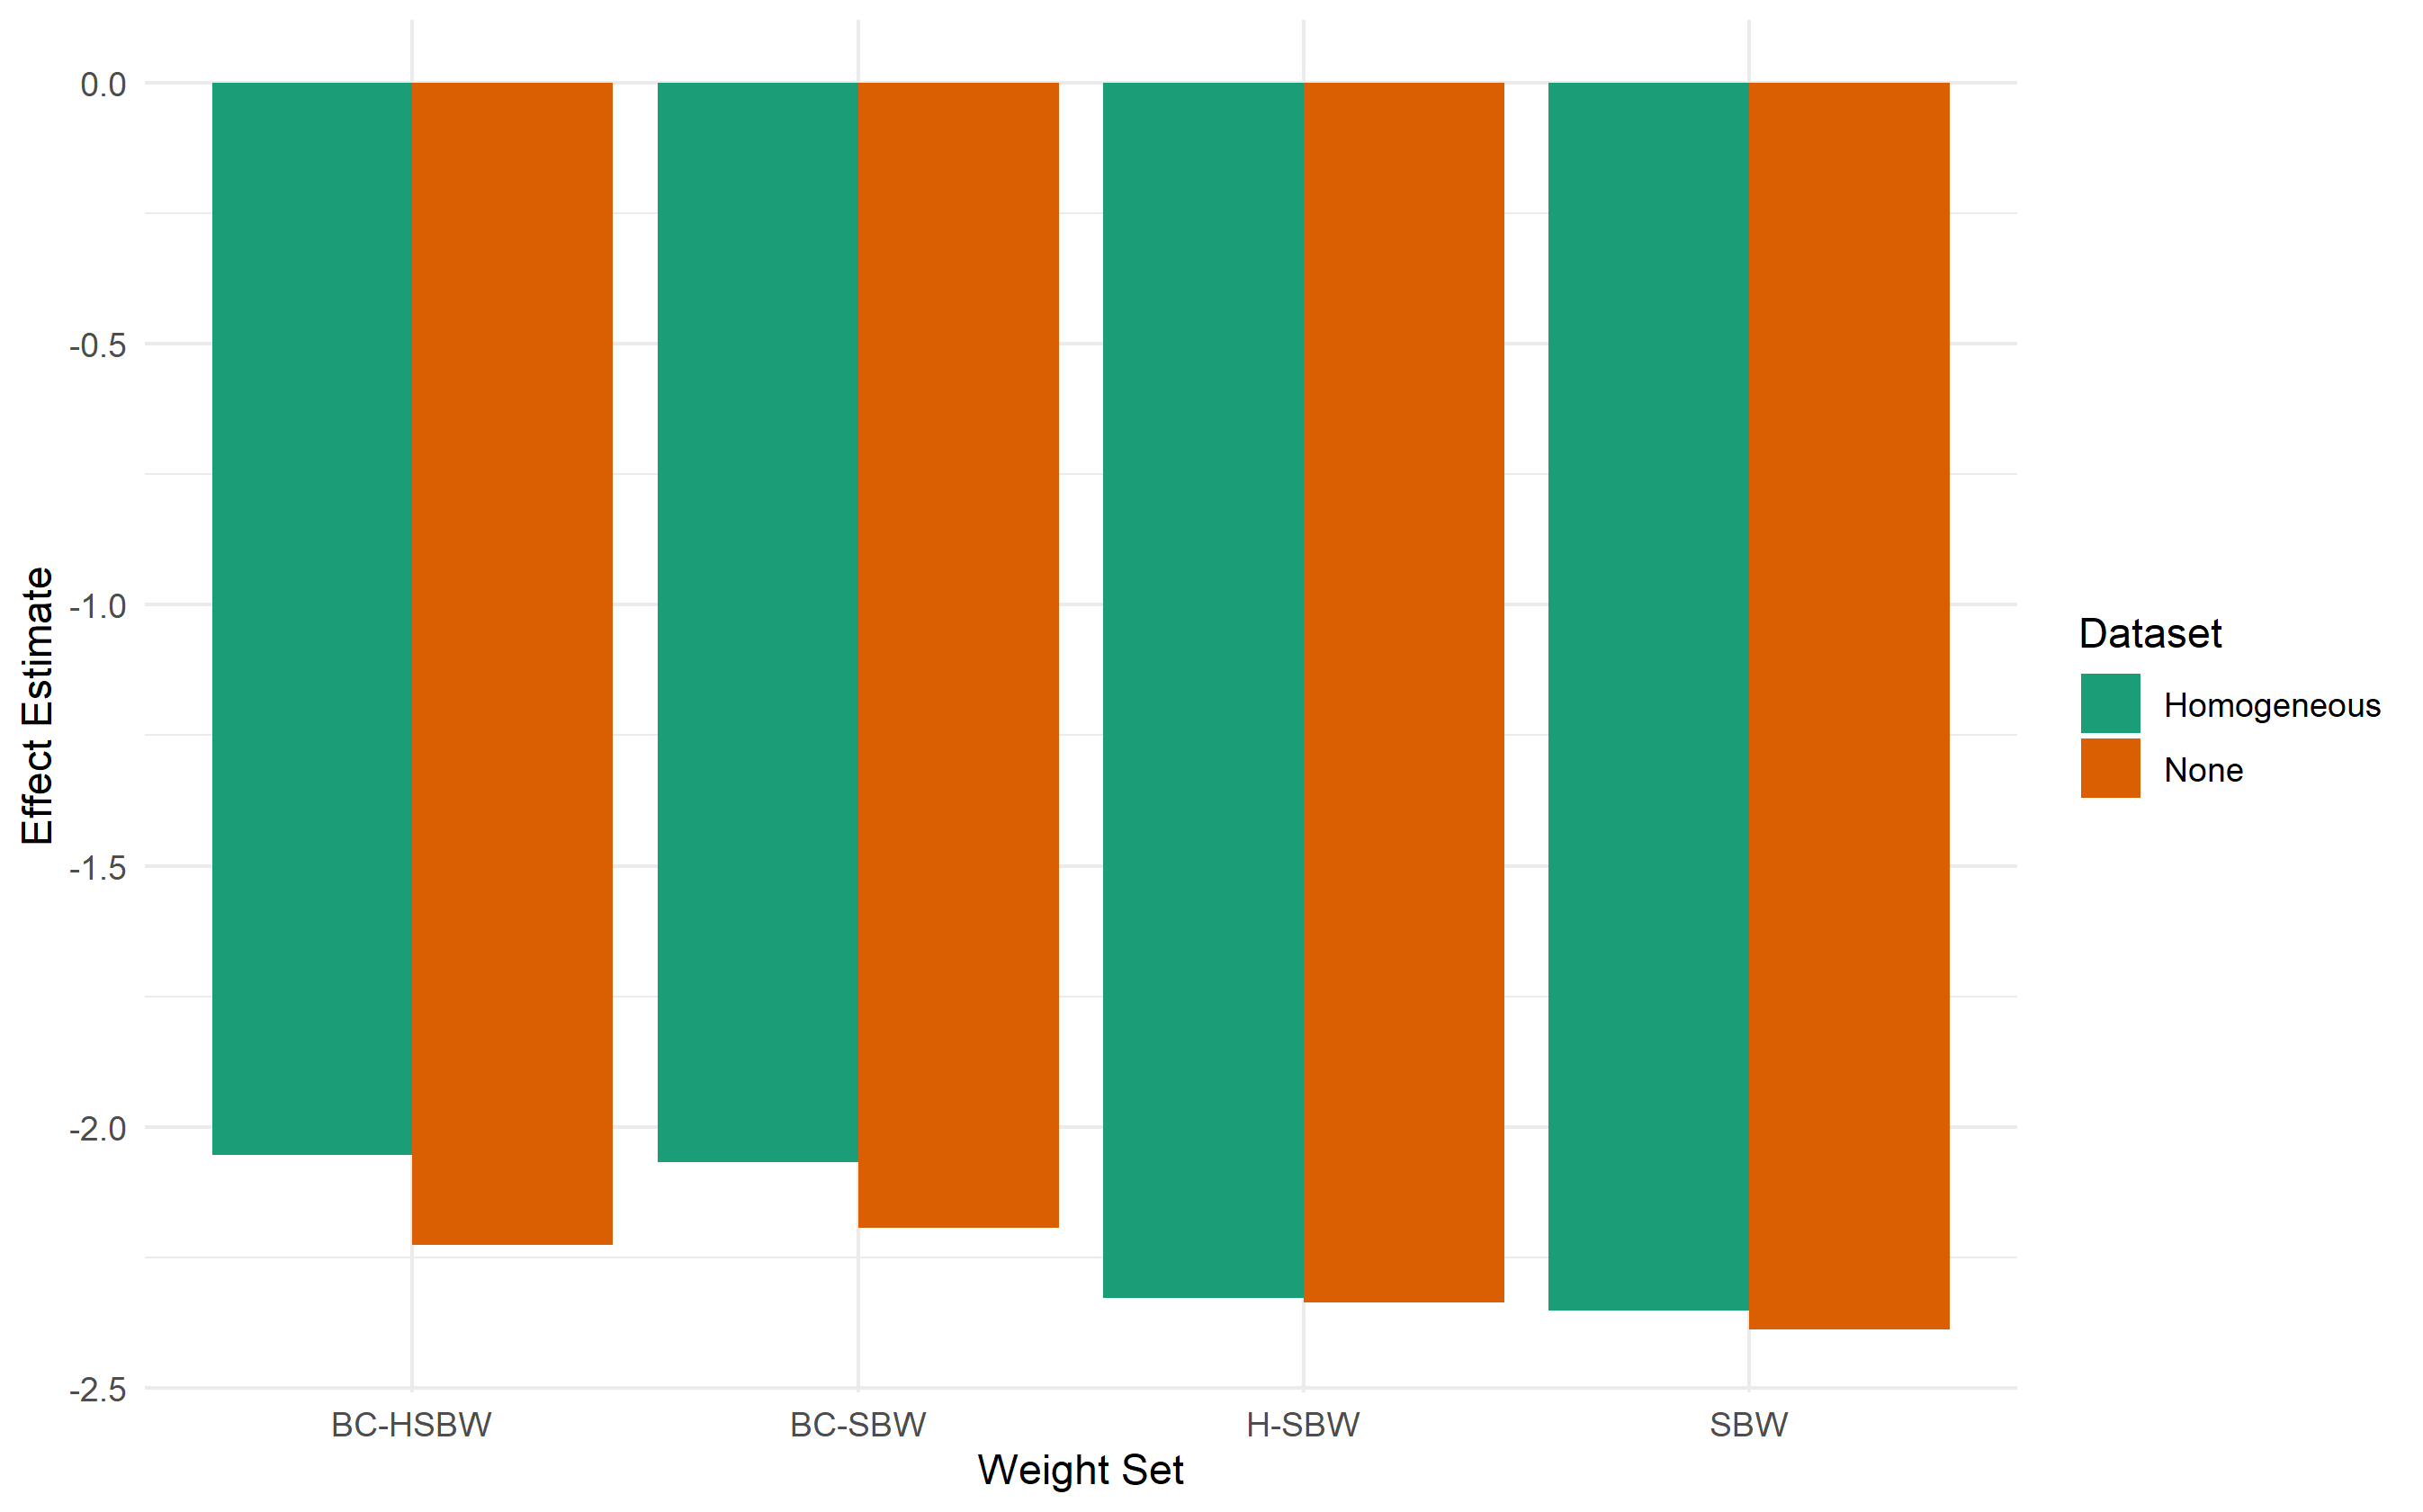
\includegraphics[scale=0.6]{01_Plots/point-estimates-c1.png}
\end{center}
\end{figure}

Lastly, we examine the robustness of our point estimates to the removal of individual states (these are the same point estimates used to calculate our confidence intervals). Figure~\ref{fig:loostateplot} shows how the point estimates for each estimator changes for both the (homogeneous) adjusted and unadjusted datasets. We see similar results in either case: removing Ohio tends to move the point estimates farther from zero (though the change is larger on the adjusted dataset). By contrast, removing North Dakota, Kentucky, or California tends to move the estimates closer to zero. 

\begin{figure}[H]
\begin{center}
    \caption{Estimator sensitivity to states}
    \label{fig:loostateplot}
    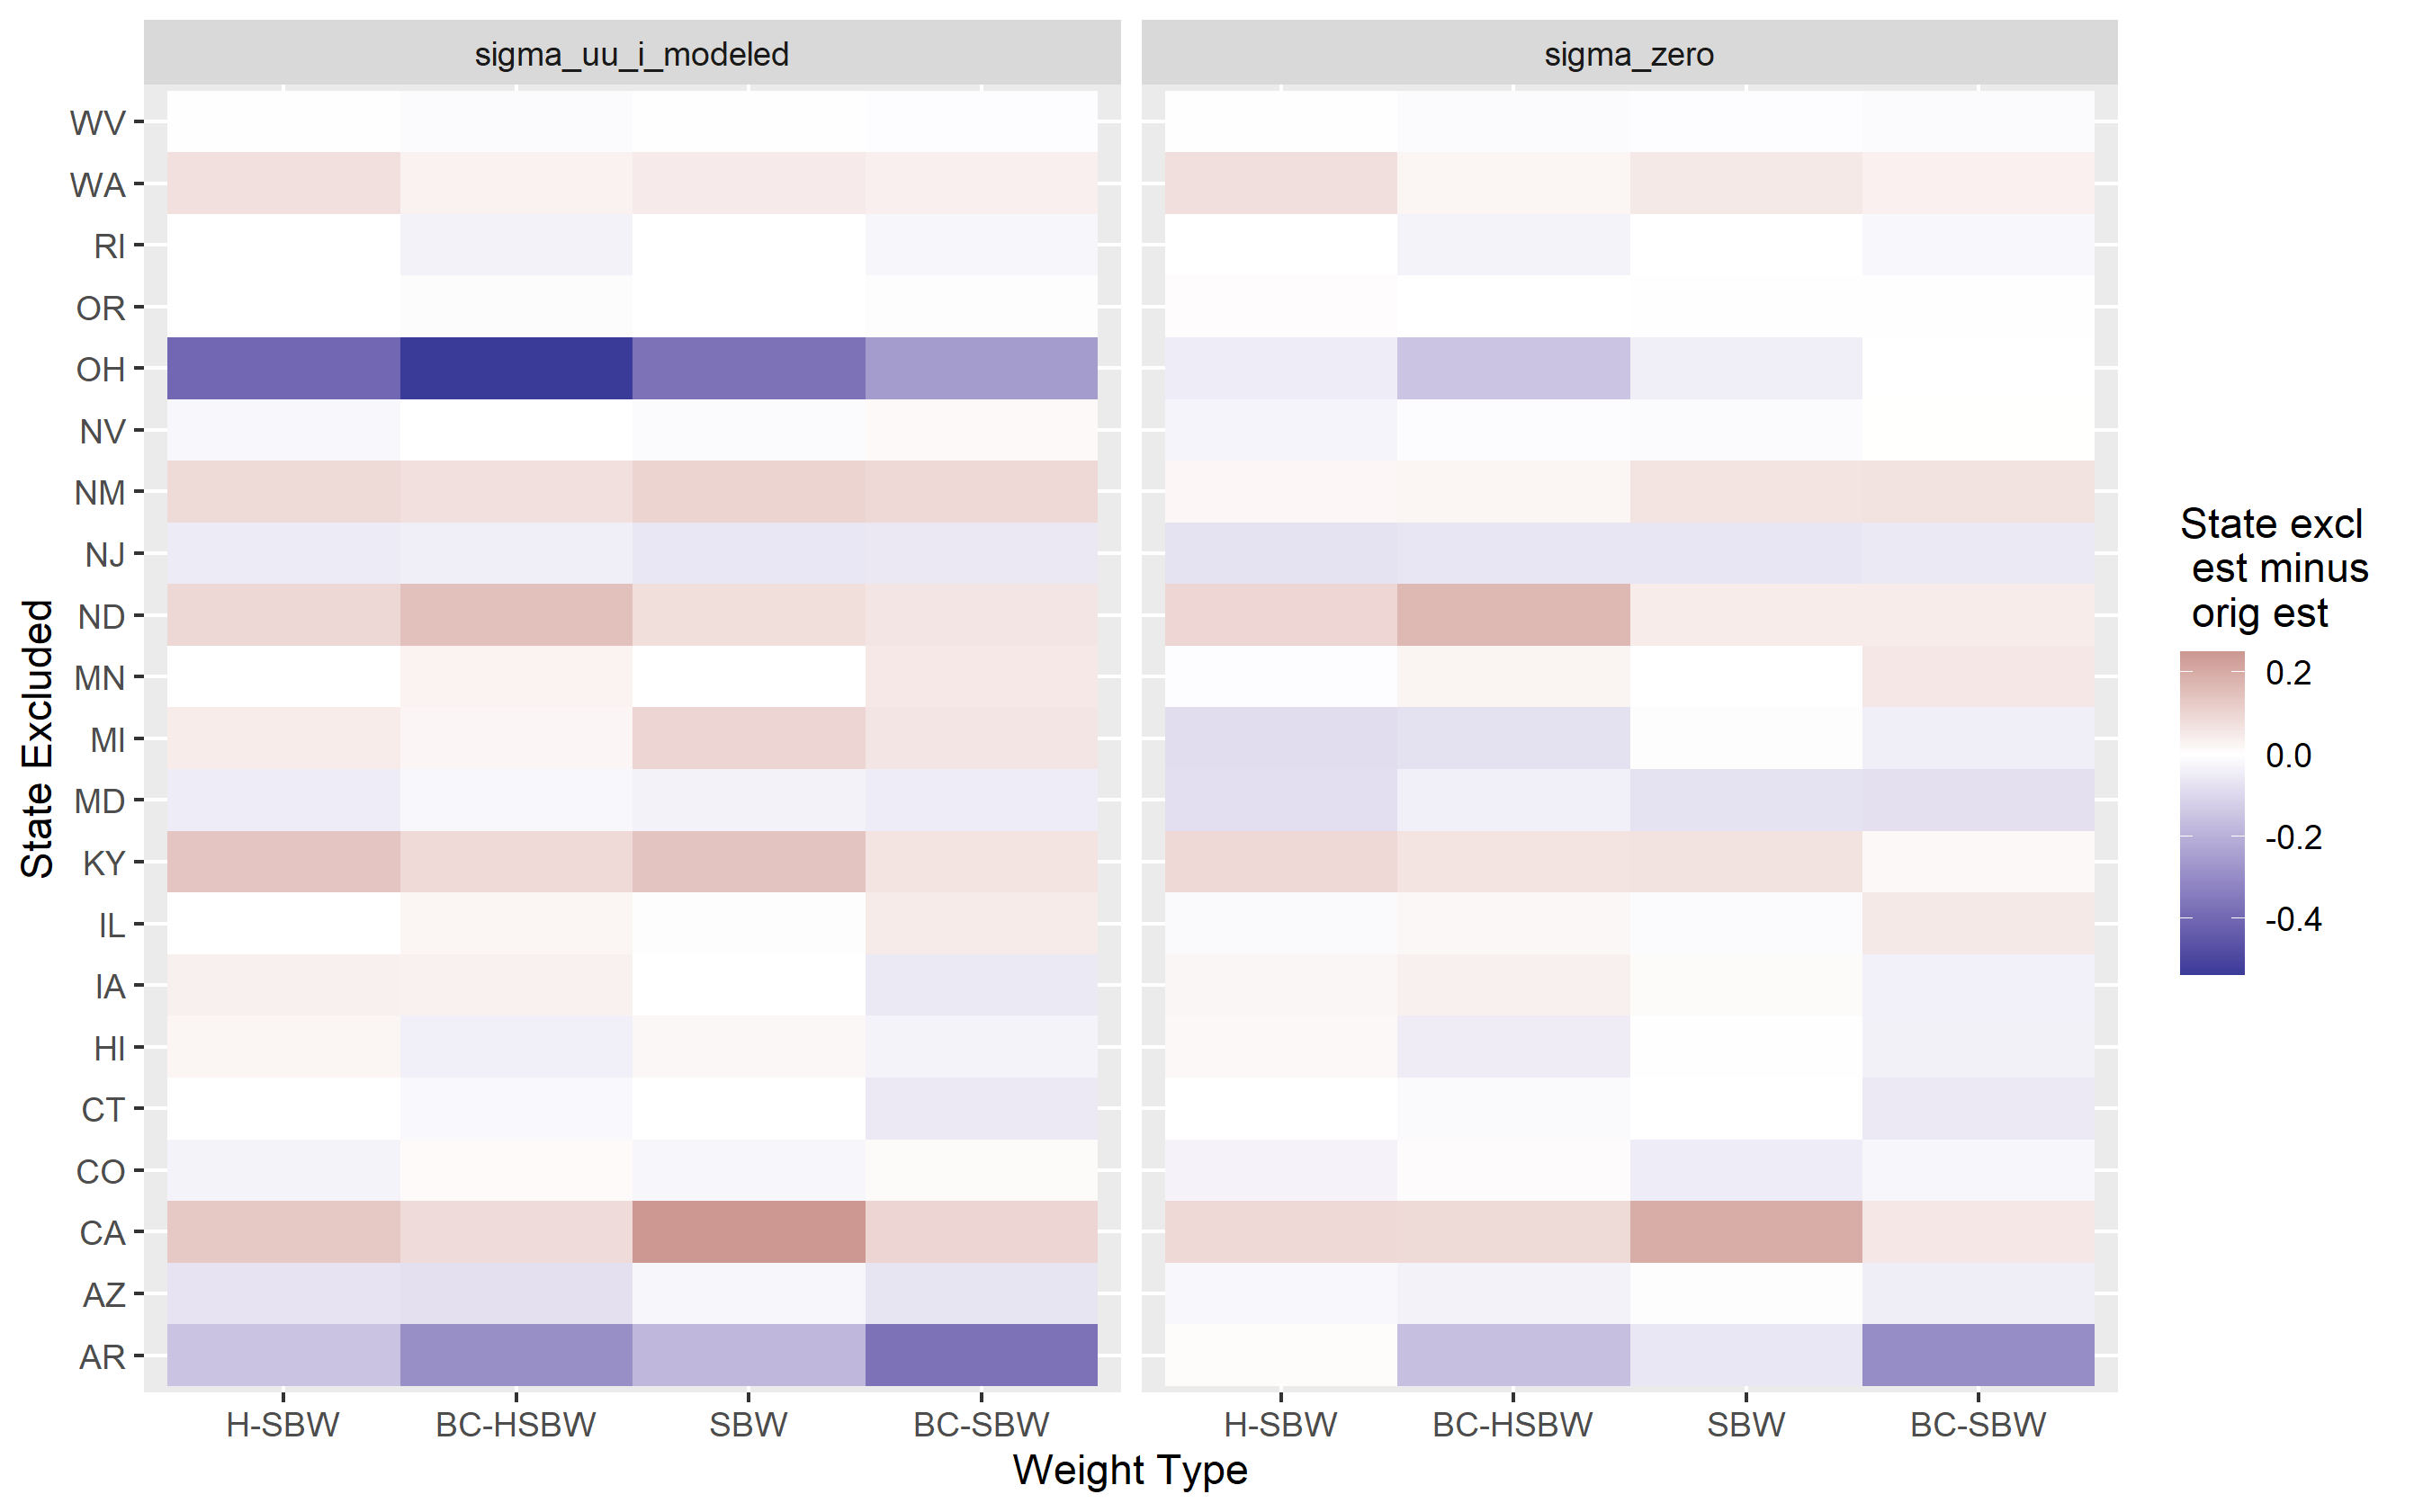
\includegraphics[scale=0.6]{01_Plots/loostate-sensitivityc1-state-uu-i.png}
\end{center}
\end{figure}

\subsection{Sensitivity analysis} \label{sssec:sensitivity}

We now consider the sensitivity of our analysis with respect to no anticipatory treatment effects. Several states had partial limited expansions prior to 2014. Following \cite{frean2017premium}, these states are California, Connecticut, Minnesota, New Jersey, and Washington. We rerun our analyses excluding CPUMAs from all five of these states. We have no a priori expectation about how removing these states might affect our estimates: on the one hand, states that expanded early might have a smaller treatment effect after 2014 because they already enrolled newly eligible individuals. On the other hand, if these states were also more motivated to enroll people in Medicaid, they might have experienced larger post-expansion coverage gains. Figure~\ref{fig:weightsbystatec2} in Appendix D displays the H-SBW weights summed by state alongside BC-HSBW, which extrapolates to reduce the imbalances. 

Excluding early expansion states, we estimate an effect of -2.09 (-2.85, -1.33) percentage points using H-SBW weights and -2.05 (-2.75, -1.35) percentage points for SBW. These estimates are quite similar to though slightly closer to zero than the the primary estimates. We also see that the differential between these estimates and the unadjusted estimates is slightly larger: -2.28  (-2.82, -1.74) percentage points for H-SBW and -2.21 (-2.71, -1.72) percentage points for SBW. 

When we add the bias-correction the point estimates again move closer to zero: -1.94 (-2.96, -0.92) percentage points for BC-HSBW and -1.99 (-3, -0.99) percentage points for BC-SBW. Overall these results suggests that the results are relatively robust to the exclusion of these states, so that potential violations of this causal assumption do not appear to be a large factor.

\subsection{Covariate importance}

We also investigate our hypothesis that factors associated with Governance are associated with treatment response. As discussed above, we first remove the balance constraints on the Republican governance indicators and estimate $\hat{\psi}^1_v$, and then subtract our original ETC point estimate from this quantity to generate $\hat{\Delta}_v^1$. Because this quantity does not reflect a clear population target, instead of confidence intervals, we present the minimum and maximum leave-one-state-out values in parentheses next to the original estimate.

For the H-SBW estimator we calculate $\hat{\Delta}^1$ equal to -0.69 (min = -0.83, max = -0.42) and equal to -0.79 (min = -0.90, max = -0.66) on our unadjusted dataset. In other words, our primary estimated treatment effect moved 0.78 percentage points further away from zero when we excluded the Republican governance indicators. This reflects a 33 percent decrease in our point estimate, a not-unsubstantial difference. Moreover, all of these estimates were less than zero, regardless of whether we conditioned on the covariate adjustment or not, regardless of whether we remove the early expansion states or not, and when removing each state. Across all specifications that we ran the minimum change we calculated was -1.34 and the maximum was -0.36. Additional distributional results across all leave-one-state-out estimates are available in Appendix E, Table~\ref{tab:rdiffc1}. Figure~\ref{fig:repub} displays our estimates of $\hat{\Delta}_v^1$ on our primary dataset and removing early expansion states (conditional on the covariate adjustment). 

We also consider four other covariate sets. We find that our estimates are most sensitive to controlling for pre-treatment outcomes and unemployment rates. This is not unexpected: all else equal, the expansion region had much lower pre-treatment uninsurance rates. If we do not control for these covariates, the comparable region will likely have lower pre-treament uninsurance rates, causing the estimated counterfactual to be closer to zero. The effect estimates were less sensitive to the removal of other covariate groups, and all point estimates are available in Appendix E, Table~\ref{tab:ptests}.

\begin{figure}[H]
\begin{center}
    \caption{Removing Republican Governance Indicators}
    \label{fig:repub}
    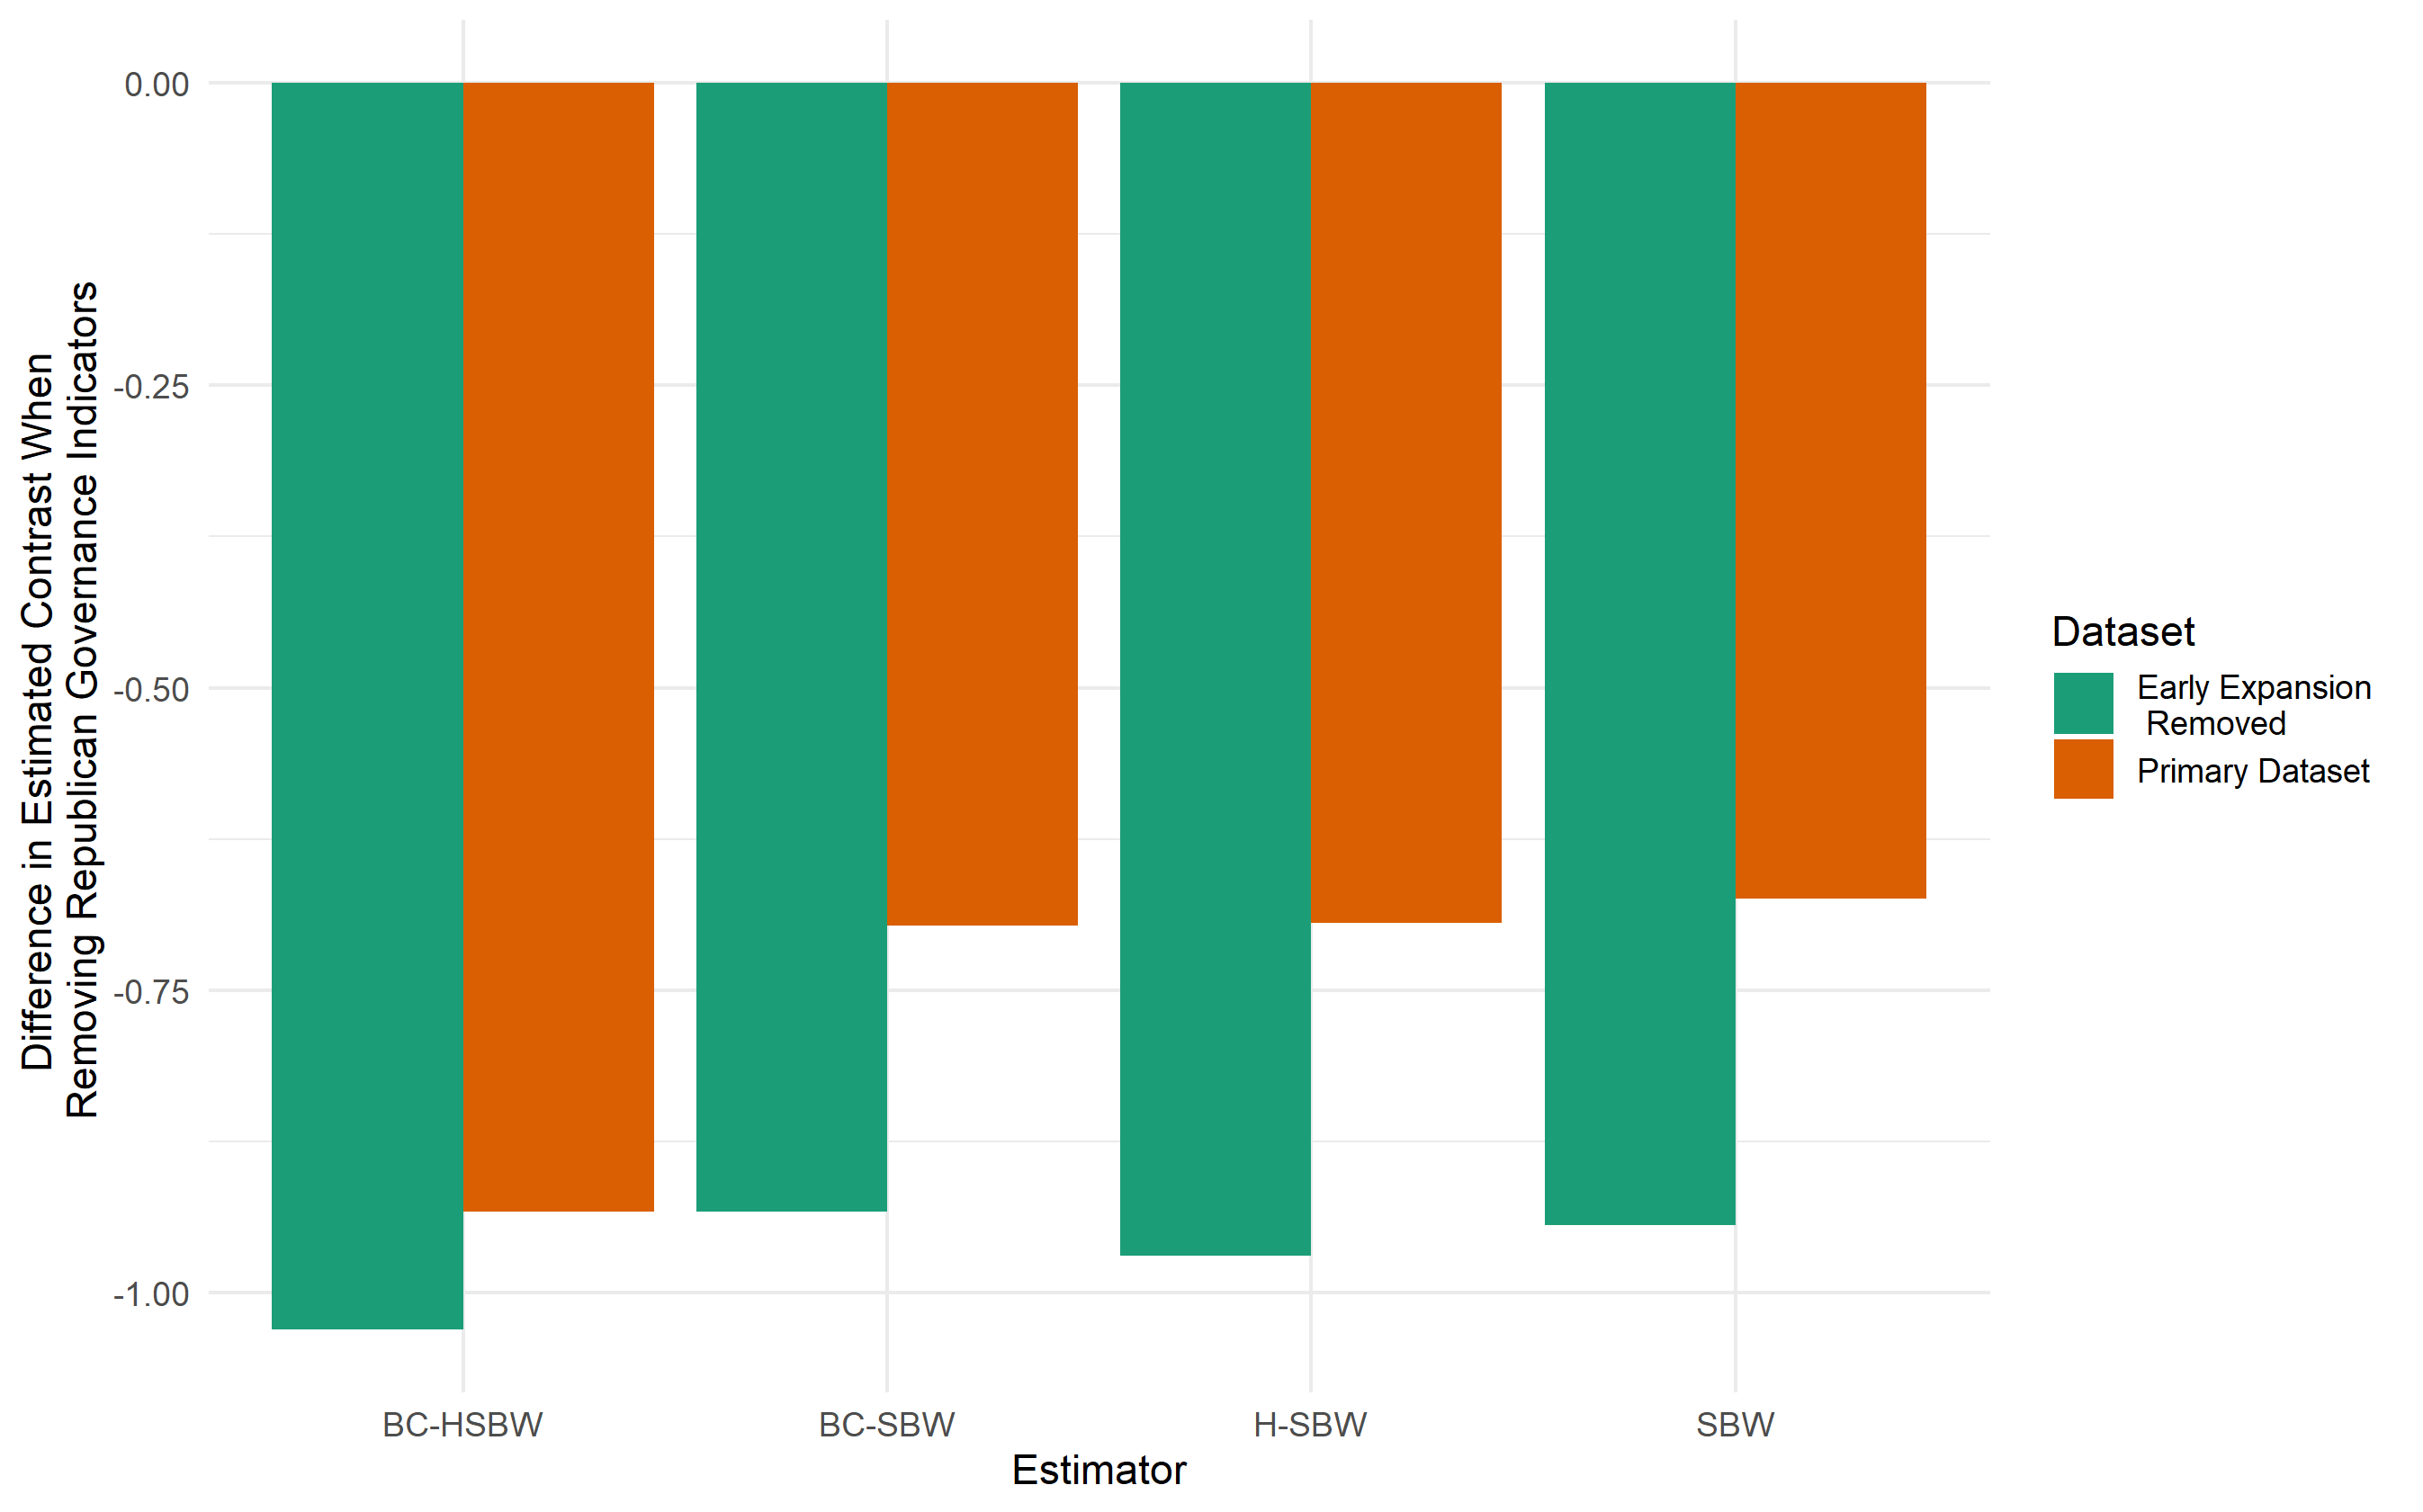
\includegraphics[scale=0.6]{01_Plots/repub-diff-all-estimators.png}
\end{center}
\end{figure}

These results highlight the importance of Republican governance in our counterfactual outcome model of $Y^1$. If the models specified by \cite{kaestner2017effects} and \cite{courtemanche2017early} are correct (that is, they correctly omit Republican governance from their balancing weights for estimating $Y^0$), this would suggest treatment effect heterogeneity with respect to Republican governance. Moreover, because the expansion-state region is much more Democratic than the non-expansion region, this heterogeneity could potentially drive differences between the ETC and the ETT.

Since this is a policy question of some interest, we directly investigate this by estimating the outcome model on the full data with treatment assignment interacted with each covariate \footnote{For this analysis we calculate separate covariate adjustments on the untreated data. The summary statistics for this adjustment are available in Appendix D.}. We then examine how the estimated treatment effect would change if we decreased the interaction between treatment assignment and each Republican governance indicator -- Republican governor, Republican lower legislature control, and Republican total control -- by 50 percentage points (note that the original variables are either 0 or 100 and measured at the state level). This linear combination of coefficients estimates how the treatment effect would change for any given collection of states against a set that is identical except for being 50 percentage points lower, on average, across the Republican governance indicators. However, we do not find that this linear combination is statistically significant on either the adjusted or unadjusted datasets. That is, we do not find evidence of treatment effect heterogeneity with respect to Republican governance (though this analysis does not rule out this possibility either).

\section{Discussion}
We estimate that had states that did not expand Medicaid in 2014 instead expanded their programs, they would have seen a -2.33 (-3.49, -1.16) percentage point change in the adult uninsurance rate. Existing estimates place the ETT between -3 and -6 percentage points. These estimates vary depending on the targeted sub-population of interest, the data used, the level of modeling (individuals or regions), and the modeling approach (see, e.g., \cite{courtemanche2017early}, \cite{kaestner2017effects}, \cite{frean2017premium}). We find that our estimate of the ETC is closer to zero than these ETT estimates. This difference may be a function of these different modeling strategies, or it may suggest that the ETC is smaller in absolute magnitude than the ETC. Our results do highlight the importance of controlling for Republican governance when generating our counterfactual estimate, which may drive our treatment effect estimate closer towards zero relative to the ETT; however, our investigation into treatment effect heterogeneity is ultimately statistically inconclusive. Regardless, due to the potential for effect heterogeneity, we emphasize the importance of directly estimating the targeted counterfactual of interest, and being explicit about the assumptions used to estimate these quantities. We now consider our methodological contributions, study limitations, and we conclude by considering the policy implications of these findings.

\subsection{Methodological considerations}

Our study makes several methodological contributions to the literature on synthetic controls and balancing weights. First, we clarify some of the assumptions required to extend the synthetic controls literature to estimate the treatment effect on the controls. The key challenge is that we need to predict treatment response rather than the outcome absent treatment. We argue that we cannot use pre-treatment outcomes to conduct variable selection without strong assumptions about the relationship between the counterfactual outcome models. In brief, estimating the ETC is an arguably more difficult problem because it requires a priori understanding of which covariates likely predict treatment response. We emphasize there may exist covariates that are not confounders of the outcome absent treatment, but that may be important confounders of the outcome under treatment, and that using pre-treatment outcomes to conduct variable selection risks missing these covariates. We use Republican governance as an example of this in our application, which \cite{kaestner2017effects} and \cite{courtemanche2017early} do not balance in their synthetic control weights in their studies of the effects of Medicaid expansion on uninsurance rates. By contrast we show that failing to control for this factor in our models leads to substantially larger treatment effect estimates, indicating their confounding role in our counterfactual model.\footnote{We caution that in actuality these covariates may also be confounders of the outcome absent treatment, and our failure to conclusively show effect heterogeneity with respect to this covariate supports this.} While perhaps obvious, this point does not seem to have yet been appreciated in the applied literature. For example, \cite{born2020lockdowns} recently used synthetic controls to estimate Sweden's COVID cases and deaths had they instituted a lockdown. The authors balance on pre-treatment infections, urbanization rate, and population size. Yet they do not explicitly argue why these covariates are the most relevant determinants of the potential outcome model under treatment, or what assumptions they are relying on that their model should be a good counterfactual model.

Second, our estimation procedure illustrates the H-SBW objective, which can improve upon the SBW objective when using hierarchical data. Assuming the errors in the outcome model follow the covariance structure posited by \cite{kloek1981ols}, H-SBW produces a lower variance estimator by more evenly dispersing weights across states. Our results illustrate this property (see, e.g, Figure~\ref{fig:sbwvhsbw1}). The assumption underlying the particular structure of our objective is that our model errors have constant variance and constant within-state correlation $\rho$. However, our procedure requires assuming the covariance structure and $\rho$ in advance. We choose $\rho = 0.2$ for this application; however, it would be interesting to come up with a data-driven approach to choose this tuning parameter (or perhaps for the covariance structure in general). 

Third, our estimation procedure accounts for measurement error in our covariates. We modify the constraint set to balance on a linear approximation to the true covariate values using regression-calibration techniques (\cite{gleser1992importance}). In Table~\ref{tab:balcomp} we show that the weights calculated on the unadjusted dataset fail to achieve the desired level of covariate balance on the adjusted dataset. Specifically, we find that the weighted pre-treatment outcomes may be lower than we wanted, which we speculate may bias our treatment effect downward. When we compared our estimates using the adjusted covariates to the unadjusted covariates, we find that our point estimates decrease (although often only slightly) in absolute magnitude. Essentially, when generate weights on the unadjusted data to estimate the 2014 counterfactual outcome, they are fitting to noise, causing the weighted region to suffer from regression to the mean. This can make our treatment effect estimates appear larger in absolute magnitude than they should be. Once we adjust for the measurement error, our point estimates decrease in absolute magnitude (see also \cite{daw2018matching}, who discuss this phenomenon in more detail in the context of difference-in-differences designs). Overall, our study provides a roadmap for future studies that may wish to correct for potential measurement error while using balancing weights. 

One caveat is that we did not attempt to calibrate our procedure to navigate an optimal bias-variance tradeoff with respect to the measurement error. It is possible that this procedure was sub-optimal with respect to the mean-square error of our estimator. In particular, the bias induced by the measurement error decreases with square root of the sample size used to calculate each CPUMAs covariate values, the minimum of which were over three hundred. Meanwhile, the variance of our counterfactual estimate should decrease with the square root of the number of treated states (of which there are 22). From a theoretical perspective, the variance is of a larger order than the bias; moreover, adjusting for the bias will further increase the variance of the estimator. These concerns are consistent with our observed results. We find that our variance estimates are an order of magnitude larger than the changes in our point estimates when we adjust our data, and that our variance estimates typically increase more than the point estimates changes once we account for the measurement error. 

\subsection{Limitations}

Our study is not without methodological limitations. We first caution that we required strong modeling assumptions throughout. In particular, we require SUTVA, no anticipatory treatment effects, no unmeasured confounding conditional on the true covariates, and several parametric assumptions about both the outcome and measurement error models. We were able to address some concerns about possible violations of these assumptions. For example, our results were fairly robust to the exclusion of possible ``early expansion states'', and to different weighting strategies (including positivity restrictions, extrapolation, and overlap weights). We also examined two versions of our covariate adjustment and found similar results with either. Even when we run our procedures on the unadjusted covariates the point estimates change, our results do not change qualitatively. However, we do not attempt to address concerns about SUTVA violations, particularly the impact of spillovers across regions. And while we believe that no unmeasured confounding is reasonable for this problem, we did conduct any sensitivity analyses with respect to this assumption.

A second limitation pertains to interpreting our results against the existing literature. As we noted above, each study is idiosyncratic with respect to the data used, the targeted population of interest, the modeling choices, and level of analysis. To attempt to make our study comparable with existing work, we follow the covariates, study period, and data used most closely by \cite{courtemanche2017early}, who calculate an ETT estimate of -3.1 percentage points. However, we note two key differences between our studies. First, \cite{courtemanche2017early} modeled individual-level data, while we model CPUMA-level aggregates. Second, we exclude several states from our expansion pool while \cite{courtemanche2017early} include all states and DC in their analysis. As a result we do not make any formal statistical claims about the differences between our estimates, or between our estimates and any other specific paper, as they could also be a function of any of these other differences in our study. Relatedly, we caution against committing the ``ecological fallacy:'' specifically, we cannot directly infer individual-level behavior from the ecological correlations in our study without much stronger assumptions (see, e.g., \cite{subramanian2009revisiting}).

\subsection{Policy considerations}

We find that our point estimates for the ETC are still somewhat smaller in absolute magnitude than existing estimates of the ETC. While we make no formal statistical claims about these differences, this finding nevertheless highlights the importance of caution when using estimates of the ETT to make inferences about the ETC. Because almost every outcome of interest is largely mediated through increasing the number of insured individuals, if the ETC is in fact different than the ETT, then projecting findings from an estimate of the ETT to the ETC may lead to inaccurate inference. For example, \cite{miller2019medicaid} study the effect of Medicaid expansion on mortality. Using their estimate of the ETT they project that had all states expanded Medicaid, 15,600 deaths would have been avoided during their study's time-period. If we believe that this number increases monotonically with the number of uninsured individuals, this estimate may be an overestimate if the ETC is less than the ETT, or an underestimate if the ETC is greater. Directly estimating the ETC can therefore also help us better model interesting downstream effects mediated through decreasing the uninsurance rate. 

\section{Conclusion}

This is the first study we are aware of that directly estimates the foregone coverage expansions of Medicaid expansion on states that did not expand Medicaid in 2014. Our estimation approach contributes to the methodological literature on synthetic controls by clarifying some of the assumptions required to use longitudinal data to estimate the ETC rather than the ETT, and to the balancing weights literature by using an estimation procedure that account for hierarchical data structure and covariates measured with error. We estimate that had states that did not expand their Medicaid eligibility requirements in 2014 done so, they would have seen a -2.33 (-3.49, -1.16) percentage point change in their uninsurance rate. This point estimate is closer to zero than existing estimates of the ETT, which range between -3 and -6 percentage points (\cite{frean2017premium}). From a practical standpoint, we caution against using using existing estimates of the ETT to make inferences about the ETC. From a policy standpoint, if the goal of Medicaid expansion is to increase access to insurance for low-income adults, state and federal policy-makers may wish to consider policies that make Medicaid enrollment easier if not automatic.



\begin{appendix}

\import{Text_files}{/proof}

\section{Adjustment Details}

We provide additional details about estimating $\eta_a$, allowing separate adjustment for both the control and treated data.\footnote{We only use $\hat{\eta}_0$ for estimating the ETT as a sensitivity check. Our primary estimates only rely on $\hat{\eta}_1$.} We begin by estimating the unit-level covariance matrices $\Sigma_{vv, sc}$, the sampling variability for each CPUMA, by using the individual replicate survey weights to generate $b = 80$ additional CPUMA-level datasets. We then estimate $\Sigma_{vv, sc}$:

\begin{equation}
\hat{\Sigma}_{vv, sc} = \frac{4}{80}\sum_{b=1}^{80}(W_{b, sc} - \bar{W}_{sc})(W_{b, sc} - \bar{W}_{sc})^T
\end{equation}

where the $4$ in the numerator comes from the process used to generate the replicate survey weights and $\bar{W}_{sc}$ is the vector of covariate values estimated using the original ACS weights.

In contrast to our proof in Section~\ref{ssec:proof}, we do not assume that $\Sigma_{XX \mid A = a}$ or $\Sigma_{vv \mid A_s = a}$ are equal across values of $a$. Instead we let $\hat{\Sigma}_{WW \mid A = a} = n_a^{-1}\sum_{sc: A_s = a} (W_{sc} - \bar{W}_a)(W_{sc} - \bar{W}_a)^T$. This estimator is calculated on the original observed dataset. We then estimate $\Sigma_{XX \mid A = a}$ using:

\begin{equation}
\hat{\Sigma}_{XX \mid A = a} = \hat{\Sigma}_{WW \mid A = a} - n_a^{-1}\sum_{sc: A_s = a} \hat{\Sigma}_{vv, sc}
\end{equation}

Define

\begin{equation}
\hat{\kappa}_a = \hat{\Sigma}_{WW \mid A = a}^{-1}\hat{\Sigma}_{XX \mid A = a}
\end{equation}

Notice that $\hat{\kappa}_a$ is a matrix of estimated coefficients of a linear regressions of the (unobserved) matrix $X_{sc}$ on (observed) matrix $W_{sc}$. We can then estimate $X_{sc}$ using $\hat{\eta}_a(W_{sc})$: 

\begin{equation}
\hat{\eta}_a(W_{sc}) = \bar{W}_a + \hat{\kappa}_a^T(W_{sc} - \bar{W}_a)
\end{equation}

where $\bar{W}_a = n_a^{-1}\sum_{sc: A_s = a} W_{sc}$. We call this the ``homogeneous adjustment'' and note that this approximately aligns with the adjustments suggested by \cite{carroll2006measurement} and \cite{gleser1992importance}. 

We also consider a second estimate that we call the ``heterogeneous adjustment.'' This adjustment accounts for the fact that some regions with large populations are estimated quite precisely, while regions with small populations are estimated much less precisely (additionally, for a given CPUMA, some covariates are measured using three years of data, and others only one). 

For this adjustment we model an individual-level $\Sigma_{vv, sc}$ as a function of the sample sizes used to estimate each covariate. In particular, let $s_{sc}$ be the q-dimensional vector of the sample sizes used to estimate each covariate value for a given CPUMA. Let $\matr{S}_{sc} = \sqrt{s_{sc}}\sqrt{s_{sc}}^T$. We assume that $\sqrt{s_{sc}} \odot v_{sc} \sim N(0, \Sigma_{vv, a})$. We then know that $\Sigma_{vv, sc}^m = \Sigma_{vv, a} \oslash \matr{S}_{sc}$ (where we add the superscript $m$ to distinguish that this individual-level covariance matrix comes from a common model).

To estimate these matrices we pool our initial estimates of the CPUMA-level covariance matrices within each treatment group ($\hat{\Sigma}_{vv, sc}$) to generate $\hat{\Sigma}_{vv, a} = n_a^{-1}\sum_{sc: A_s = a} \matr{S}_{sc} \circ \Sigma_{vv, sc}$. We estimate $\hat{\Sigma}_{vv, sc}^m = \hat{\Sigma}_{vv, a} \oslash \matr{S}_{sc}$. From this we estimate $\hat{\Sigma}_{XX \mid A = a} = \hat{\Sigma}_{WW \mid A = a} - n_a^{-1}\sum_{sc: A_s = a}\hat{\Sigma}_{vv, sc}$. Finally, we calculate $\hat{\kappa}_{sc} = (\hat{\Sigma}_{XX \mid A = a} + \hat{\Sigma}_{vv, sc}^m)^{-1}\hat{\Sigma}_{XX \mid A = a}$, which we use to estimate $\hat{\eta}_{sc}$. We can then use these CPUMA-level covariate matrices to estimate $X_{sc}$ from $W_{sc}$.

This adjustment accounts for CPUMA-level variability in the measurement error, and should more greatly affect outlying values of imprecisely estimated covariates, while leaving precisely estimated covariates closer to their observed value in the dataset. Moreover, we are able to use the full efficiency of using all units in the modeling. On the other hand, this model assumes that all differences in the sampling variability are due to the sample sizes, and assumes away heterogeneity due to heteroskedasticity. A second cost is that in practice, as shown in Appendix~\ref{sec:appendixsumstat}, we find that this adjustment, compared to the homogeneous approach, is more likely to lead to extreme values of $\hat{\eta}(W_{sc})$ that fall outside of the support of the original data. This may not be true generally, but is a problem for this application. 

\section{Summary Statistics and Covariates}\label{app:sumstats}

In this section we display summary statistics about the CPUMA-level datasets. The first two tables pertain to treatment assignment classifications. Table~\ref{tab:txassign} lists the states that are assigned to each group: the first two columns include the treatment states and control states in our primary analysis. The third column lists the treatment states for our sensitivity analysis that excludes ``early expansion'' states. The final column indicates states that were always excluded from the analysis. Table~\ref{tab:cpumasperstate} displays the total number of CPUMAs per state, as well as a column reiterating the state's treatment assignment and whether it was an early expansion state.

The subsequent tables and figure display summary information about the expansion state data and the homogeneous and heterogeneous covariate adjustments detailed in Appendix~\ref{app:adjustmentdetails}. 

Table~\ref{tab:summarytab1} displays univariate summary statistics for the treated CPUMAs. Specifically, the table displays mean, interquartile range, and the range (as defined by the maximum value minus the minimum value) for the unadjusted dataset, the heterogeneous adjustment, and the homogeneous adjustment. We see that the covariate adjustments generally reduce the variability relative to the unadjusted data. 

Table~\ref{tab:extreme1} displays the frequency that the adjusted covariates fell outside of the support of the unadjusted dataset on our primary dataset. The frequency is comparable for either adjustment and the counts are low, supporting the use of the linear model outlined in \eqref{eqn:regcal}. We also calculate these adjustments excluding early expansion states, and recalculate these adjustments excluding each state one at a time to calculate our variance estimates, yielding different results with respect to the quality of the resulting adjustments. These results are available on request.

Table~\ref{tab:timetrends} displays the trends in the outcome over time by treatment group. We use these estimates to compute the difference-in-differences estimator of the ETT in footnote \ref{footnote_did}. 

Figure~\ref{fig:corrmatrix} displays the Pearson's correlation coefficients for the bivariate relationships between the covariates on the unadjusted dataset (including both treated and untreated units). These point estimates may be biased due to the measurement error in the covariates. Nevertheless, this matrix is useful for at least two reasons: first, assuming the correlations among the treated and untreated units are similar, the more heavily correlated the data the easier it should be to attain covariate balance (see, e.g., \cite{d2021overlap}). This matrix gives a general sense of how correlated the data are, even if the estimates are biased. Second, these correlations can suggest potential confounders by revealing which variables are most heavily associated with treatment assignment and the pre-treatment outcomes. For example, the plot shows a strong association between Republican governance and treatment assignment, and a smaller association between these variables with pre-treatment outcomes. The plot also illustrates strong associations between the pre-treatment uninsurance rates, though they are more weakly associated with treatment assignment. 

\begin{table}[h!]\caption{Treatment assignment classification}\label{tab:txassign}
\centering
\hline 
\begin{tabularx}{\textwidth}{XXXX} \\ 
Treated states & Control states & Early expansion states & Always excluded \\ 
\hline
AR, AZ, CA, CO, CT, HI, IA, IL, KY, MD, MI$^\textrm{a}$, MN, ND, NJ, NM, NV, OH, OR, RI, WA, WV & AK, AL, FL, GA, ID, IN, KS, LA, ME, MO, MS, MT, NC, NE, OK, PA, SC, SD, TN, TX, UT, VA, WI, WY & CA, CT, MN, NJ, WA & DE$^\textrm{c}$, MA$^\textrm{c}$, NH$^\textrm{b}$, NY$^\textrm{c}$, VT$^\textrm{c}$, DC$^\textrm{c}$\\ 
\hline 
\end{tabularx} {
     \vspace{1ex} }
     {\par \raggedright $^\textrm{a}$ Expanded April 2014 \par 
     \raggedright $^\textrm{b}$ Expanded September 2014; included for covariate adjustment estimates but not as a possible weight donor for treatment effect estimates \par 
    \raggedright $^\textrm{c}$ Comparable coverage policies prior to 2014 
    \par}
\end{table}

\begin{table}[ht]
\centering
\caption{Number of CPUMAs per state}\label{tab:cpumasperstate}
\begin{tabular}{lllrl}
  \hline
State Full & State & Treatment & Number CPUMAs & Early Expansion \\ 
  \hline
Delaware & DE & Excluded &   4 & No \\ 
  Massachusetts & MA & Excluded &  15 & No \\ 
    New Hampshire & NH & Excluded $^\textrm{a}$ &   4 & No \\ 
  New York & NY & Excluded & 123 & No \\ 
  Vermont & VT & Excluded &   4 & No \\ 
  Arizona & AZ & Expansion &  11 & No \\ 
  Arkansas & AR & Expansion &  15 & No \\ 
  Colorado & CO & Expansion &  15 & No \\ 
  Hawaii & HI & Expansion &   8 & No \\ 
  Illinois & IL & Expansion &  47 & No \\ 
  Iowa & IA & Expansion &   7 & No \\ 
  Kentucky & KY & Expansion &  23 & No \\ 
  Maryland & MD & Expansion &  36 & No \\ 
  Michigan & MI & Expansion &  44 & No \\ 
  Nevada & NV & Expansion &   7 & No \\ 
  New Mexico & NM & Expansion &   6 & No \\ 
  North Dakota & ND & Expansion &   2 & No \\ 
  Ohio & OH & Expansion &  44 & No \\ 
  Oregon & OR & Expansion &  17 & No \\ 
  Rhode Island & RI & Expansion &   6 & No \\ 
  West Virginia & WV & Expansion &   4 & No \\ 
  California & CA & Expansion & 110 & Yes \\ 
  Connecticut & CT & Expansion &  22 & Yes \\ 
  Minnesota & MN & Expansion &  27 & Yes \\ 
  New Jersey & NJ & Expansion &  38 & Yes \\ 
  Washington & WA & Expansion &  22 & Yes \\ 
  Alabama & AL & Non-expansion &  18 & No \\ 
  Alaska & AK & Non-expansion &   4 & No \\ 
  Florida & FL & Non-expansion &  59 & No \\ 
  Georgia & GA & Non-expansion &  20 & No \\ 
  Idaho & ID & Non-expansion &   1 & No \\ 
  Indiana & IN & Non-expansion &  24 & No \\ 
  Kansas & KS & Non-expansion &   9 & No \\ 
  Louisiana & LA & Non-expansion &  15 & No \\ 
  Maine & ME & Non-expansion &   5 & No \\ 
  Mississippi & MS & Non-expansion &   7 & No \\ 
  Missouri & MO & Non-expansion &  16 & No \\ 
  Montana & MT & Non-expansion &   1 & No \\ 
  Nebraska & NE & Non-expansion &  11 & No \\ 
  North Carolina & NC & Non-expansion &  27 & No \\ 
  Oklahoma & OK & Non-expansion &   8 & No \\ 
  Pennsylvania & PA & Non-expansion &  55 & No \\ 
  South Carolina & SC & Non-expansion &  10 & No \\ 
  South Dakota & SD & Non-expansion &   1 & No \\ 
  Tennessee & TN & Non-expansion &  28 & No \\ 
  Texas & TX & Non-expansion &  49 & No \\ 
  Utah & UT & Non-expansion &   8 & No \\ 
  Virginia & VA & Non-expansion &  15 & No \\ 
  Wisconsin & WI & Non-expansion &  21 & No \\ 
  Wyoming & WY & Non-expansion &   2 & No \\ 
   \hline
\end{tabular}
     \vspace{1ex}
     \newline
     {\raggedright $^\textrm{a}$ Included for covariate adjustment estimates but not as a possible weight donor for treatment effect estimates \par }
\end{table}

\begin{table}[h!]
\centering
\caption{Univariate summary statistics on adjusted data, primary dataset \\ (Mean, IQR, Range)}\label{tab:summarytab1}
\begin{tabular}{rllll}
  \hline
Variable & Unadjusted & Heterogeneous & Homogeneous \\ 
  \hline
  Age: 19-29 Pct & (24.5, 6, 30.9) & (24.5, 5.9, 29) & (24.5, 5.9, 29) \\ 
  Age: 30-39 Pct & (20.9, 3.4, 20.9) & (20.9, 3.1, 19.1) & (20.9, 3.1, 19.4) \\ 
  Age: 40-49 Pct & (22.2, 2.5, 15.4) & (22.2, 2.3, 13.7) & (22.2, 2.2, 13.7) \\ 
  Avg Adult to Household Ratio & (151, 27.2, 174.3) & (151, 27.2, 173.8) & (151, 27.2, 173.3) \\ 
  Avg Pop Growth & (100.3, 1.9, 13.7) & (100.3, 1.2, 6.2) & (100.3, 1.2, 6.5) \\ 
  Children: Missing Pct & (10.5, 6.6, 41) & (10.5, 6.5, 40.8) & (10.5, 6.5, 40.5) \\ 
  Children: One Pct & (11.1, 3.1, 14.3) & (11.1, 2.8, 12.3) & (11.1, 2.8, 12.5) \\ 
  Children: Three or More Pct & (5.2, 2, 14.1) & (5.2, 1.7, 13.5) & (5.2, 1.7, 13.3) \\ 
  Children: Two Pct & (9.7, 3.5, 15) & (9.7, 3.3, 13.5) & (9.7, 3.2, 13.6) \\ 
  Citizenship Pct & (90, 11.9, 57.1) & (90, 11.8, 55.4) & (90, 11.7, 55.7) \\ 
  Disability Pct & (10.5, 5.3, 28.6) & (10.4, 5.3, 26.7) & (10.5, 5.4, 27.2) \\ 
  Educ: HS Degree Pct & (26.3, 10.7, 43.2) & (26.3, 10.6, 41.8) & (26.3, 10.6, 42) \\ 
  Educ: Less than HS Pct & (11.4, 7.7, 45.3) & (11.4, 7.5, 45) & (11.4, 7.4, 44.6) \\ 
  Educ: Some College Pct & (33.5, 7.9, 34.2) & (33.5, 7.5, 32.9) & (33.5, 7.4, 33) \\ 
  Female Pct & (50.1, 1.6, 15.4) & (50.1, 1.4, 14.2) & (50.1, 1.5, 14.2) \\ 
  Foreign Born Pct & (18.1, 22.4, 76) & (18.1, 22.2, 75.2) & (18.1, 22.2, 75.4) \\ 
  Hispanic Pct & (15.9, 17.7, 97.2) & (15.9, 17.7, 97) & (15.9, 17.7, 97) \\ 
  Inc Pov: $<$ 138 Pct & (20, 11.9, 45.6) & (20, 11.8, 44.8) & (20, 11.8, 43.9) \\ 
  Inc Pov: 139-299 Pct & (24.9, 8.4, 34.2) & (24.9, 7.9, 34.2) & (24.9, 7.8, 34.1) \\ 
  Inc Pov: 300-499 Pct & (23.6, 5.5, 23) & (23.6, 4.9, 22.2) & (23.6, 4.9, 22.2) \\ 
  Inc Pov: 500 + Pct & (29.3, 18.5, 69.1) & (29.3, 18.5, 68.1) & (29.3, 18.5, 68) \\ 
  Married Pct & (50.7, 9.4, 45.1) & (50.7, 9, 44.1) & (50.7, 9.1, 44.2) \\ 
  Race: White Pct & (73.8, 25.4, 91.9) & (73.8, 25.5, 91.7) & (73.8, 25.5, 91.8) \\ 
  Republican Governor 2013 $^\textrm{a}$& (31.1, 100, 100) & (31.1, 100, 100) & (31.1, 100, 100) \\ 
  Republican Lower Leg Control 2013 $^\textrm{a}$ & (24.1, 0, 100) & (24.1, 0, 100) & (24.1, 0, 100) \\ 
  Republican Total Control 2013 $^\textrm{a}$ & (19.8, 0, 100) & (19.8, 0, 100) & (19.8, 0, 100) \\ 
Student Pct & (11.7, 3.4, 29.5) & (11.7, 3.5, 28.1) & (11.7, 3.5, 28) \\ 
  Unemployed Pct 2011 & (10.2, 4.6, 25.5) & (10.2, 3.9, 23.8) & (10.2, 3.9, 22.5) \\ 
  Unemployed Pct 2012 & (9.4, 4.5, 28.3) & (9.4, 4.3, 23.6) & (9.4, 4.3, 23.5) \\ 
  Unemployed Pct 2013 & (8.4, 3.6, 23.4) & (8.4, 3.5, 20.1) & (8.4, 3.5, 20.5) \\ 
  Uninsured Pct 2011 & (19.6, 11.2, 59) & (19.7, 10.9, 51.8) & (19.6, 10.9, 52.5) \\ 
  Uninsured Pct 2012 & (19.4, 9.9, 50.6) & (19.4, 10.1, 49.7) & (19.4, 10.3, 50.2) \\ 
  Uninsured Pct 2013 & (19, 11.2, 49.9) & (19, 10.3, 48.2) & (19, 10.5, 48.7) \\ 
  Urban Pct $^\textrm{b}$ & (82.9, 31.3, 91.3) & (82.9, 31.3, 91.3) & (82.9, 31.3, 91.3) \\ 
   \hline
\end{tabular}
     \vspace{1ex}
     
     {\raggedright $^\textrm{a}$ Derived from data obtained from National Conference of State Legislatures \par
     $^\textrm{b}$ Derived from 2010 Census \par
     }
\end{table}

\begin{table}[h!]
\centering
    \caption{Frequency of covariate adjustments falling outside the support of the unadjusted data \newline (primary dataset)}
    \label{tab:extreme1}
\begin{tabular}{lll}
  \hline
Variables & Heterogeneous & Homogeneous \\ 
  \hline
Age: 19-29 Pct & 0 & 0 \\ 
  Age: 30-39 Pct & 0 & 0 \\ 
  Age: 40-49 Pct & 0 & 0 \\ 
  Avg Adult to Household Ratio & 0 & 0 \\ 
  Citizenship Pct & 1 & 0 \\ 
  Disability Pct & 2 & 2 \\ 
  Educ: HS Degree Pct & 0 & 0 \\ 
  Educ: Less than HS Pct & 1 & 1 \\ 
  Educ: Some College Pct & 0 & 0 \\ 
  Female Pct & 0 & 0 \\ 
  Foreign Born Pct & 1 & 1 \\ 
  Uninsured Pct 2011 & 0 & 0 \\ 
  Uninsured Pct 2012 & 1 & 1 \\ 
  Uninsured Pct 2013 & 0 & 1 \\ 
  Hispanic Pct & 0 & 0 \\ 
  Inc Pov: $<$ 138 Pct & 1 & 1 \\ 
  Inc Pov: 139-299 Pct & 1 & 1 \\ 
  Inc Pov: 300-499 Pct & 0 & 0 \\ 
  Inc Pov: 500 + Pct & 0 & 0 \\ 
  Married Pct & 0 & 0 \\ 
  Children: Missing Pct & 1 & 1 \\ 
  Children: One Pct & 0 & 0 \\ 
  Avg Pop Growth & 0 & 0 \\ 
  Race: White Pct & 1 & 1 \\ 
  Student Pct & 0 & 0 \\ 
  Children: Three or More Pct & 2 & 1 \\ 
  Children: Two Pct & 1 & 1 \\ 
  Unemployed Pct 2011 & 0 & 0 \\ 
  Unemployed Pct 2012 & 0 & 0 \\ 
  Unemployed Pct 2013 & 0 & 0 \\ 
   \hline
\end{tabular}
\end{table}

\begin{table}[ht]
\centering
\caption{Mean non-elderly adult uninsurance rates, 2009-2014}\label{tab:timetrends}
\begin{tabular}{lrrrrrr}
  \hline
Treatment Group & 2009 & 2010 & 2011 & 2012 & 2013 & 2014 \\ 
  \hline
Non-expansion & 21.84 & 22.97 & 22.72 & 22.41 & 22.01 & 19.07 \\ 
  Expansion (primary dataset) & 19.52 & 20.20 & 19.63 & 19.42 & 19.01 & 14.02 \\ 
  Expansion (early excluded) & 19.40 & 20.08 & 19.21 & 19.01 & 18.55 & 13.64 \\ 
   \hline
\end{tabular}
\end{table}

\begin{figure}[h!]
\begin{center}
    \caption{Correlation matrix: full data, unadjusted covariates \newline (primary dataset)}
    \label{fig:corrmatrix}
    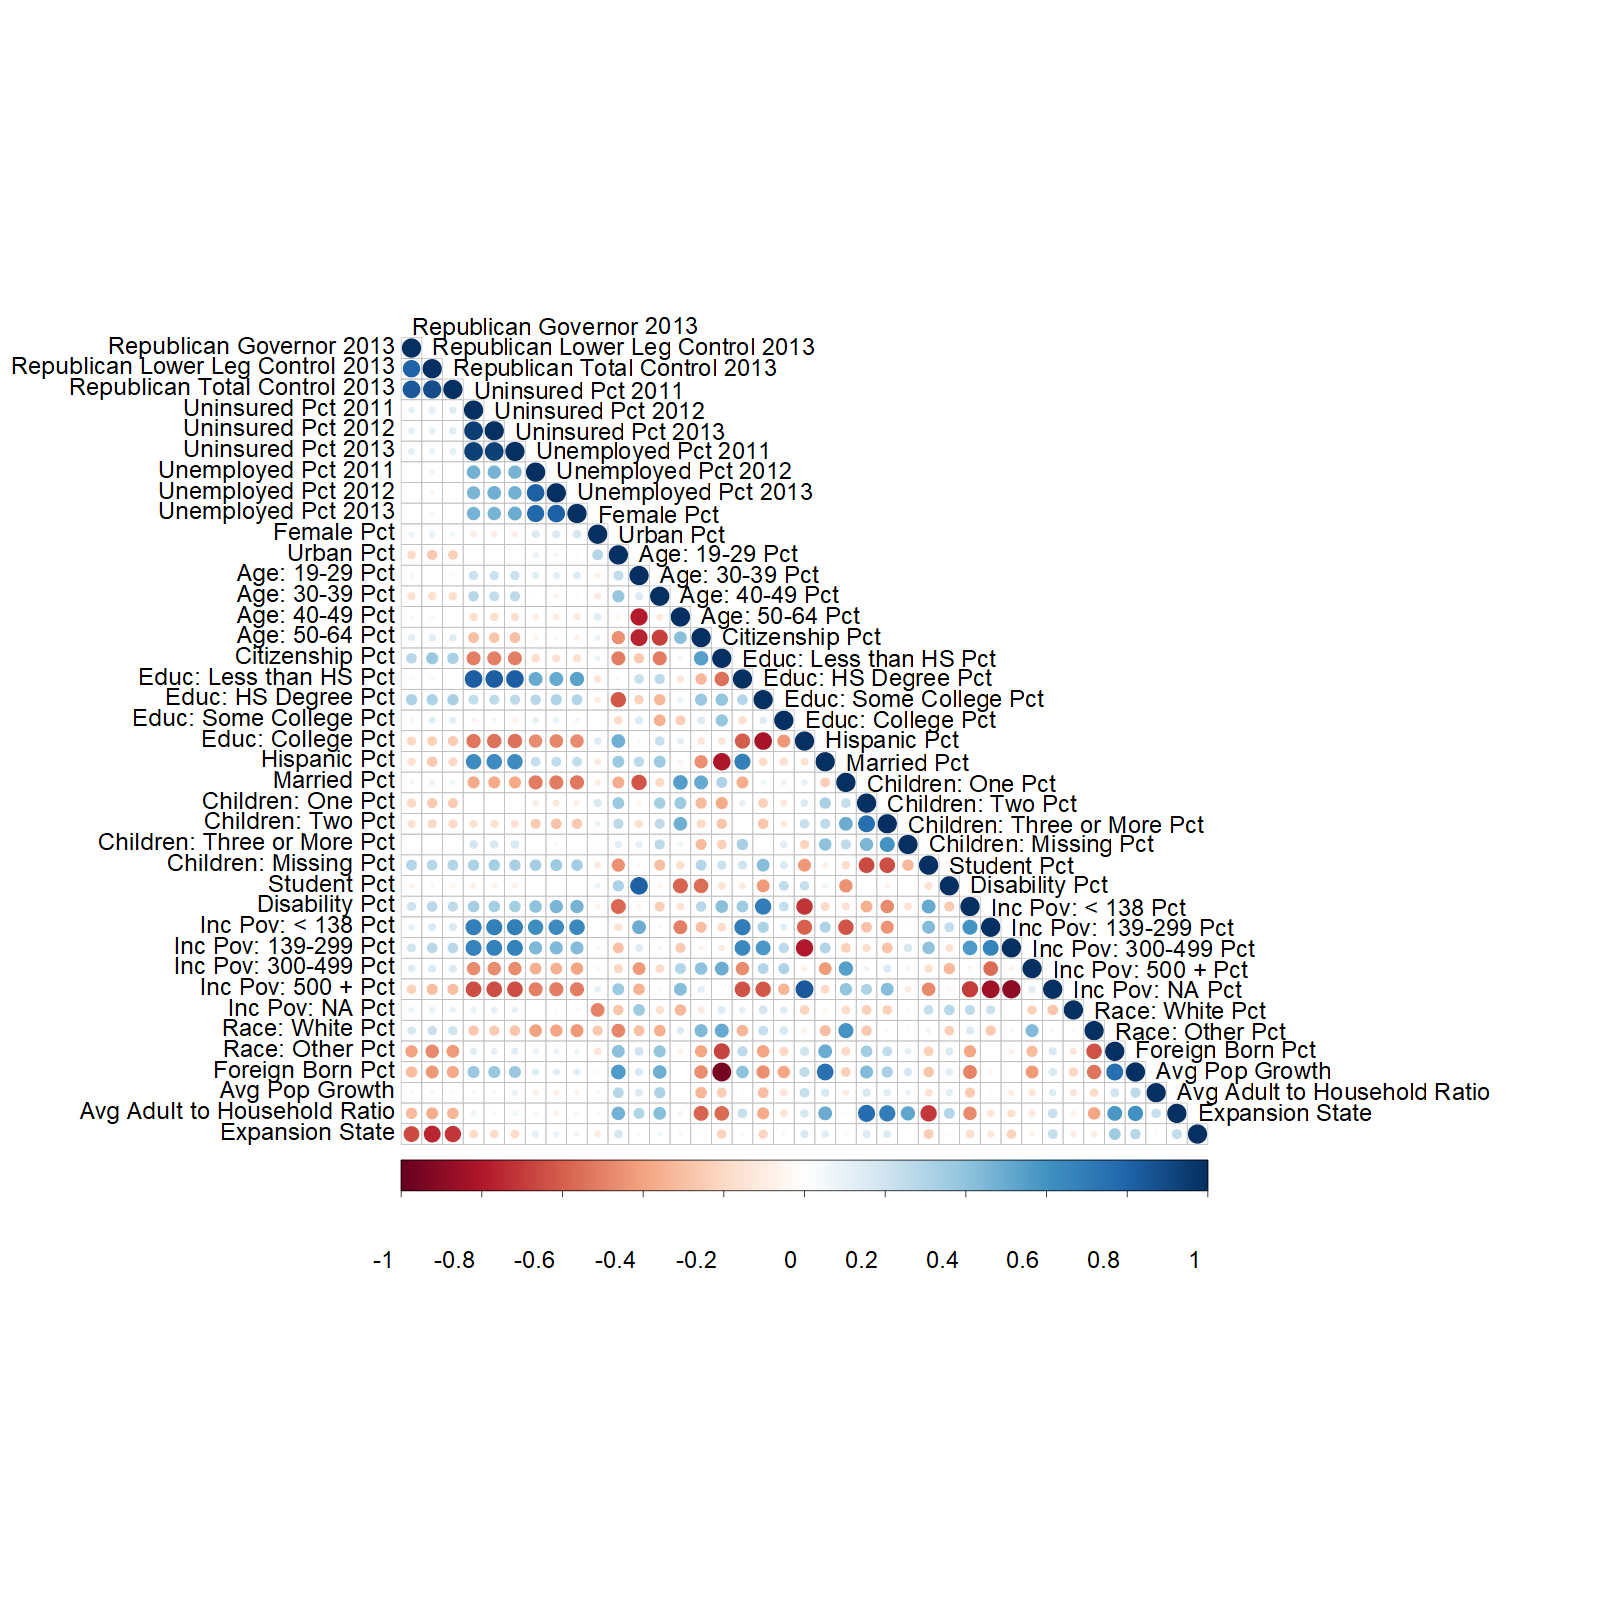
\includegraphics[scale=0.25]{01_Plots/correlation-plot-c1-sigma-zero.png}
\end{center}
\end{figure}

\clearpage

\begin{landscape}

\section{Weight Diagnostics}
\label{ssec:balancetables}

Table~\ref{tab:baltab1} displays the differences between the weighted mean covariate values of the expansion region and the mean of the non-expansion region for our primary dataset and with the early expansion states excluded (calculated using our the homogeneous covariate adjustments). The weights presented here are for the H-SBW estimator. The values under each column are in the following format: (unweighted difference, weighted difference). ``Primary'' and ``Early excluded'' refer to the primary dataset and those that exclude the early expansion states. ``Percent'' indicates that the differences displayed are in percentage points while ``Standardized'' indicates that the standardized mean differences are displayed. Additional results are available on request.

\begin{table}[h!]
\centering
    \caption{Balance table: percent and standardized mean differences, H-SBW weights}
    \label{tab:baltab1}
\begin{tabular}{lllll}
  \hline
Variables & Preferred (Percent) & Preferred (Standardized) & Early excluded (Percent) & Early excluded (Standardized) \\ 
  \hline
Age: 19-29 Pct & (-0.34, -0.34) & (-0.05, -0.05) & (-0.62, -0.21) & (-0.09, -0.03) \\ 
  Age: 30-39 Pct & (0.36, 0.17) & (0.1, 0.05) & (-0.04, 0.32) & (-0.01, 0.09) \\ 
  Age: 40-49 Pct & (0.19, -0.3) & (0.06, -0.1) & (-0.01, -0.44) & (0, -0.15) \\ 
  Avg Adult to Household Ratio & (11.29, -0.04) & (0.37, 0) & (3.37, 0.1) & (0.13, 0) \\ 
  Citizenship Pct & (-3.61, -1.59) & (-0.33, -0.15) & (-0.24, -1.45) & (-0.03, -0.16) \\ 
  Disability Pct & (-1.45, 0.52) & (-0.27, 0.1) & (-0.17, 0.63) & (-0.03, 0.11) \\ 
  Educ: HS Degree Pct & (-3.37, 0.54) & (-0.32, 0.05) & (-1.02, 0.64) & (-0.1, 0.06) \\ 
  Educ: Less than HS Pct & (-0.37, 0.83) & (-0.04, 0.1) & (-1.22, 0.76) & (-0.16, 0.1) \\ 
  Educ: Some College Pct & (-0.35, 0.4) & (-0.05, 0.06) & (0.36, 0.57) & (0.05, 0.08) \\ 
  Female Pct & (-0.34, -0.64) & (-0.16, -0.3) & (-0.25, -1) & (-0.12, -0.48) \\ 
  Foreign Born Pct & (7.6, 2) & (0.42, 0.11) & (1.02, 2) & (0.07, 0.13) \\ 
  Uninsured Pct 2011 & (-3.08, 0.05) & (-0.28, 0) & (-3.51, -0.05) & (-0.34, 0) \\ 
  Uninsured Pct 2012 & (-3, -0.05) & (-0.27, 0) & (-3.4, 0.05) & (-0.33, 0) \\ 
  Uninsured Pct 2013 & (-2.99, -0.05) & (-0.27, 0) & (-3.45, -0.05) & (-0.34, 0) \\ 
  Hispanic Pct & (4.46, 1) & (0.2, 0.04) & (-1.35, 1) & (-0.07, 0.05) \\ 
  Inc Pov: $<$ 138 Pct & (-2.05, 0.63) & (-0.19, 0.06) & (-1.33, 0.12) & (-0.12, 0.01) \\ 
  Inc Pov: 139-299 Pct & (-2.45, 0.65) & (-0.35, 0.09) & (-1.53, 0.5) & (-0.23, 0.08) \\ 
  Inc Pov: 300-499 Pct & (-0.59, -0.18) & (-0.12, -0.04) & (0.28, -0.18) & (0.06, -0.04) \\ 
  Inc Pov: 500 + Pct & (5.58, -1.3) & (0.35, -0.08) & (2.9, -1.23) & (0.2, -0.08) \\ 
  Married Pct & (-0.76, -0.43) & (-0.07, -0.04) & (-0.21, -0.53) & (-0.02, -0.05) \\ 
  Children: Missing Pct & (-3.25, -1) & (-0.36, -0.11) & (-1.99, -0.1) & (-0.21, -0.01) \\ 
  Children: One Pct & (0.7, -0.14) & (0.25, -0.05) & (0.11, -0.31) & (0.04, -0.12) \\ 
  Avg Pop Growth & (-0.09, -0.21) & (-0.07, -0.18) & (-0.26, -0.19) & (-0.22, -0.16) \\ 
  Race: White Pct & (-4.02, 1) & (-0.16, 0.04) & (0.09, 1) & (0, 0.04) \\ 
  Republican Governor 2013 & (-64.78, -25) & (-1.28, -0.5) & (-54.46, -24.87) & (-1.02, -0.47) \\ 
  Republican Lower Leg Control 2013 & (-74.72, -25) & (-1.69, -0.57) & (-56.67, -23.6) & (-1.12, -0.47) \\ 
  Republican Total Control 2013 & (-71.3, -25) & (-1.45, -0.51) & (-56.47, -25) & (-1.02, -0.45) \\ 
  Student Pct & (0.25, -0.5) & (0.04, -0.08) & (0.11, -0.25) & (0.02, -0.04) \\ 
  Children: Three or More Pct & (0, -0.21) & (0, -0.08) & (-0.17, -0.26) & (-0.07, -0.11) \\ 
  Children: Two Pct & (0.76, -0.31) & (0.23, -0.09) & (0.17, -0.37) & (0.05, -0.12) \\ 
  Unemployed Pct 2011 & (0.82, 0.15) & (0.18, 0.03) & (0.68, 0.15) & (0.15, 0.03) \\ 
  Unemployed Pct 2012 & (0.63, -0.03) & (0.14, -0.01) & (0.47, -0.03) & (0.11, -0.01) \\ 
  Unemployed Pct 2013 & (0.42, -0.15) & (0.11, -0.04) & (0.22, -0.15) & (0.06, -0.04) \\ 
  Urban Pct & (8.28, -2) & (0.26, -0.06) & (2.79, -2) & (0.08, -0.06) \\ 
   \hline
\end{tabular}
    \begin{tablenotes}
      \small
      \item The values displayed in each cell are the (weighted, unweighted) differences. The columns containing ``Standardized'' reflect the standardized mean differences while ``percent'' indicates the mean differences in percentage points. The columns containing ``Preferred'' indicate that this is for our primary analysis while ``Early excluded'' is for our analysis that excludes the early expansion states.
    \end{tablenotes}
\end{table}

Figure~\ref{fig:weightsbystatec2} display the weights summed by states when excluding the early expansion states for the H-SBW and BC-HSBW estimators.

\begin{figure}[H]
\begin{center}
    \caption{Total weights summed by state, early expansion removed}
    \label{fig:weightsbystatec2}
    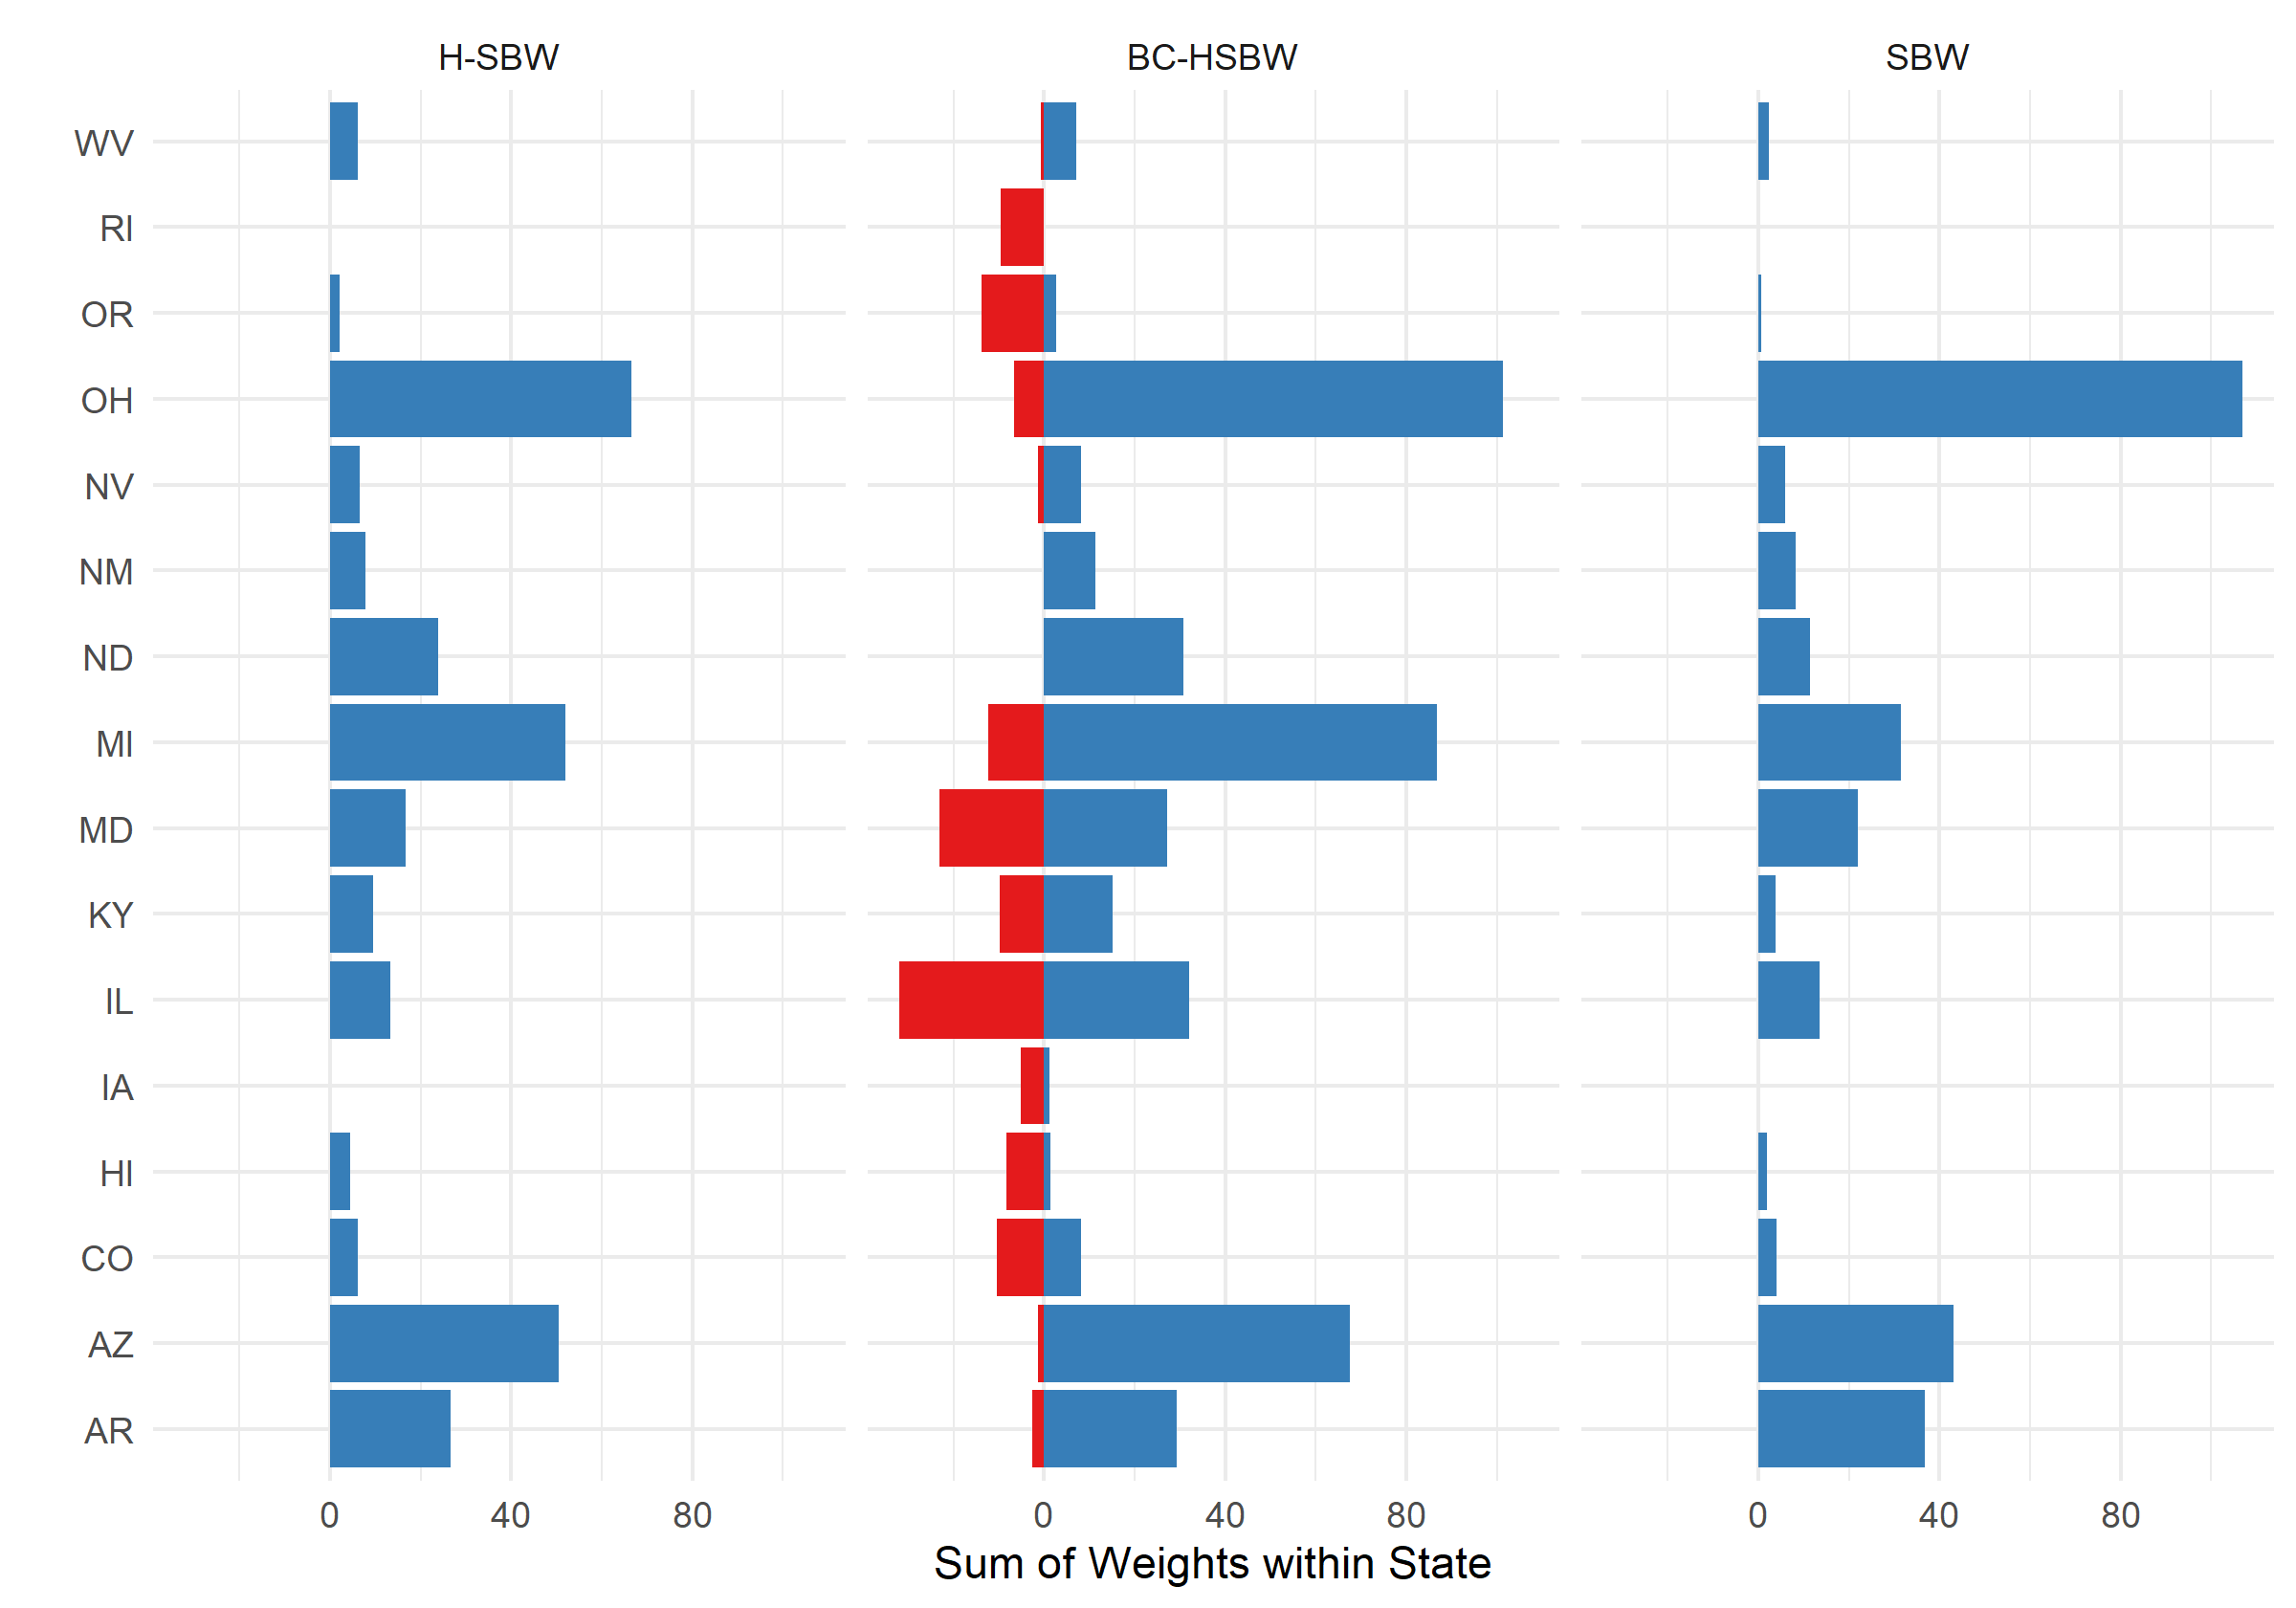
\includegraphics[scale=0.5]{01_Plots/weights-by-state-sbw-hsbw-c2-color.png}
\end{center}
\end{figure}
\end{landscape}
\clearpage

\section{Additional Results}
\label{ssec:allresults}

Table~\ref{tab:confintmain} displays the point estimates from all estimators as well as confidence intervals calculated either (a) leave-one-state-out jackknife on the adjusted dataset (CI (states)); (b) leave-one-state-out jackknife repeating the entire adjusted leaving each state out (CI (proc)). This table also includes all analyses calculated on a second version of the adjusted data where we use a common $\kappa$ for all values (sigma\_uu\_avg), which is the adjustment suggested by \cite{carroll2006measurement}. Notice that the confidence intervals are identical for ``sigma\_zero'' because this is the unadjusted dataset. ``sigma\_uu\_i'' is our preferred covariate adjustment.

\begin{table}[ht]
\centering
\caption{Point estimates and confidence intervals, primary dataset}
\label{tab:confintmain}
\begin{tabular}{llrll}
  \hline
Weight type & Sigma estimate & Psihat & CI (states) & CI (proc) \\ 
  \hline
H-SBW & sigma\_uu\_i & -2.17 & (-3.41, -0.94) & (-3.42, -0.92) \\ 
  H-SBW & sigma\_uu\_avg & -2.25 & (-3.51, -0.99) & (-3.35, -1.14) \\ 
  H-SBW & sigma\_zero & -2.35 & (-3.09, -1.61) & (-3.09, -1.61) \\ 
  BC-HSBW & sigma\_uu\_i & -2.13 & (-3.55, -0.71) & (-3.42, -0.84) \\ 
  BC-HSBW & sigma\_uu\_avg & -2.17 & (-3.57, -0.78) & (-3.39, -0.96) \\ 
  BC-HSBW & sigma\_zero & -2.40 & (-3.33, -1.46) & (-3.33, -1.46) \\ 
  SBW & sigma\_uu\_i & -2.24 & (-3.50, -0.99) & (-3.51, -0.97) \\ 
  SBW & sigma\_uu\_avg & -2.30 & (-3.67, -0.92) & (-3.45, -1.15) \\ 
  SBW & sigma\_zero & -2.40 & (-3.10, -1.69) & (-3.10, -1.69) \\ 
  BC-SBW & sigma\_uu\_i & -2.12 & (-3.15, -1.10) & (-3.11, -1.14) \\ 
  BC-SBW & sigma\_uu\_avg & -2.17 & (-3.25, -1.08) & (-3.22, -1.12) \\ 
  BC-SBW & sigma\_zero & -2.36 & (-2.93, -1.80) & (-2.93, -1.80) \\ 
   \hline
\end{tabular}
\end{table}

Table~\ref{tab:ptests} presents all point estimates from estimators that we calculated. The ``Var subset`` column indicates which variables were excluded from the estimation: 0 excludes no variables; 1 removes Republican governance indicators; 2 pre-treatment uninsurance and unemployment rates; 3 urban, age, education, citizenship, marital status, student, disability, or female; 4 race, ethnicity, income, foreign born; 5 children, population growth, and household to person ratio. We see that the largest changes generally occur when excluding the pre-treatment uninsurance and unemployment rates. This is not surprising: controlling for the other covariates, the pre-treatment uninsurance rate was substantially lower in the treated region compared to the control region. Given that pre-treatment uninsurance rates are highly correlated with post-treatment rates, we find that this comparison leads to a larger absolute magnitude point estimate, highlighting the need to control for these covariates.

%Wed Jan 13 15:24:43 2021
\begin{table}[ht]
\centering
\caption{Point estimates for all specifications}
\label{tab:ptests}
\begin{tabular}{rlrrrr}
  \hline
Variable subset & Sigma estimate & H-SBW & BC-HSBW & SBW & BC-SBW \\ 
  \hline
0 & sigma\_uu\_i & -2.17 & -2.13 & -2.24 & -2.12 \\ 
  0 & sigma\_uu\_avg & -2.25 & -2.17 & -2.30 & -2.17 \\ 
  0 & sigma\_zero & -2.35 & -2.40 & -2.40 & -2.36 \\ 
  1 & sigma\_uu\_i & -2.85 & -2.87 & -3.00 & -2.76 \\ 
  1 & sigma\_uu\_avg & -2.86 & -2.86 & -2.99 & -2.75 \\ 
  1 & sigma\_zero & -3.00 & -3.09 & -3.07 & -2.92 \\ 
  2 & sigma\_uu\_i & -5.73 & -5.05 & -5.24 & -4.70 \\ 
  2 & sigma\_uu\_avg & -5.73 & -5.05 & -5.24 & -4.70 \\ 
  2 & sigma\_zero & -5.73 & -5.13 & -5.24 & -4.77 \\ 
  3 & sigma\_uu\_i & -2.17 & -2.00 & -2.24 & -2.00 \\ 
  3 & sigma\_uu\_avg & -2.25 & -2.06 & -2.29 & -2.06 \\ 
  3 & sigma\_zero & -2.34 & -2.17 & -2.40 & -2.15 \\ 
  4 & sigma\_uu\_i & -2.35 & -2.39 & -2.29 & -2.30 \\ 
  4 & sigma\_uu\_avg & -2.39 & -2.39 & -2.32 & -2.32 \\ 
  4 & sigma\_zero & -2.45 & -2.59 & -2.43 & -2.49 \\ 
  5 & sigma\_uu\_i & -2.17 & -2.19 & -2.26 & -2.21 \\ 
  5 & sigma\_uu\_avg & -2.25 & -2.24 & -2.33 & -2.27 \\ 
  5 & sigma\_zero & -2.35 & -2.44 & -2.42 & -2.47 \\ 
   \hline
\end{tabular}
\end{table}

Table ~\ref{tab:confintmainc2} and Table~\ref{tab:secondaryptests} are identical to the structure of the previous two tables except we exclude the ``early expansion states'' from the pool of expansion state matches. 

\begin{table}[ht]
\centering
\caption{Point estimates and confidence intervals, early expansion excluded}
\label{tab:confintmainc2}
\begin{tabular}{llrll}
  \hline
Weight type & Sigma estimate & Psihat & CI (states) & CI (proc) \\ 
  \hline
H-SBW & sigma\_uu\_i & -2.05 & (-3.10, -1.00) & (-3.05, -1.05) \\ 
  H-SBW & sigma\_uu\_avg & -2.13 & (-3.20, -1.05) & (-3.17, -1.08) \\ 
  H-SBW & sigma\_zero & -2.29 & (-2.90, -1.69) & (-2.90, -1.69) \\ 
  BC-HSBW & sigma\_uu\_i & -2.14 & (-3.63, -0.64) & (-3.48, -0.80) \\ 
  BC-HSBW & sigma\_uu\_avg & -2.19 & (-3.65, -0.73) & (-3.57, -0.81) \\ 
  BC-HSBW & sigma\_zero & -2.50 & (-3.66, -1.33) & (-3.66, -1.33) \\ 
  SBW & sigma\_uu\_i & -1.91 & (-2.91, -0.91) & (-2.79, -1.03) \\ 
  SBW & sigma\_uu\_avg & -2.01 & (-3.02, -1.00) & (-2.83, -1.19) \\ 
  SBW & sigma\_zero & -2.20 & (-2.69, -1.71) & (-2.69, -1.71) \\ 
  BC-SBW & sigma\_uu\_i & -1.97 & (-3.49, -0.44) & (-3.27, -0.66) \\ 
  BC-SBW & sigma\_uu\_avg & -2.04 & (-3.59, -0.50) & (-3.39, -0.70) \\ 
  BC-SBW & sigma\_zero & -2.34 & (-3.44, -1.25) & (-3.44, -1.25) \\ 
   \hline
\end{tabular}
\end{table}

\begin{table}[ht]
\centering
   \caption{Point estimates for all specifications, early expansion excluded}
    \label{tab:secondaryptests}
\begin{tabular}{rlrrrr}
  \hline
Variable subset & Sigma estimate & H-SBW & BC-HSBW & SBW & BC-SBW \\ 
  \hline
0 & sigma\_uu\_i & -2.05 & -2.14 & -1.91 & -1.97 \\ 
  0 & sigma\_uu\_avg & -2.13 & -2.19 & -2.01 & -2.04 \\ 
  0 & sigma\_zero & -2.29 & -2.50 & -2.20 & -2.34 \\ 
  1 & sigma\_uu\_i & -2.85 & -2.99 & -2.85 & -2.86 \\ 
  1 & sigma\_uu\_avg & -2.86 & -2.98 & -2.86 & -2.86 \\ 
  1 & sigma\_zero & -3.05 & -3.18 & -2.96 & -2.99 \\ 
  2 & sigma\_uu\_i & -5.55 & -4.46 & -5.02 & -4.52 \\ 
  2 & sigma\_uu\_avg & -5.55 & -4.73 & -5.01 & -4.53 \\ 
  2 & sigma\_zero & -5.55 & -4.78 & -5.01 & -4.56 \\ 
  3 & sigma\_uu\_i & -2.05 & -2.03 & -1.91 & -1.89 \\ 
  3 & sigma\_uu\_avg & -2.13 & -2.10 & -2.00 & -1.97 \\ 
  3 & sigma\_zero & -2.27 & -2.22 & -2.20 & -2.13 \\ 
  4 & sigma\_uu\_i & -2.27 & -2.24 & -2.15 & -2.00 \\ 
  4 & sigma\_uu\_avg & -2.35 & -2.28 & -2.23 & -2.04 \\ 
  4 & sigma\_zero & -2.36 & -2.62 & -2.28 & -2.45 \\ 
  5 & sigma\_uu\_i & -2.05 & -2.20 & -1.91 & -2.03 \\ 
  5 & sigma\_uu\_avg & -2.13 & -2.26 & -1.99 & -2.11 \\ 
  5 & sigma\_zero & -2.29 & -2.45 & -2.19 & -2.36 \\ 
   \hline
\end{tabular}
\end{table}

Table~\ref{tab:loostatec1} and Table~\ref{tab:loostatec2} present point estimates for the leave-one-state out analysis for our preferred estimator, H-SBW calculated on our preferred covariate adjustment for the primary dataset and when excluding early expansion states.

\begin{table}[ht]
\centering
   \caption{Leave-one-state-out point estimates, primary dataset, preferred adjustment}
    \label{tab:loostatec1}
\begin{tabular}{lrlrl}
  \hline
State & Psihat (0) & None (states, proc) & Psihat (1) & Repub (states, proc) \\ 
  \hline
AR & -2.17 & (-2.34, -2.38) & -2.85 & (-2.81, -2.80) \\ 
  AZ & -2.17 & (-2.21, -2.24) & -2.85 & (-2.86, -2.86) \\ 
  CA & -2.17 & (-1.99, -2.02) & -2.85 & (-2.77, -2.76) \\ 
  CO & -2.17 & (-2.17, -2.23) & -2.85 & (-2.84, -2.84) \\ 
  CT & -2.17 & (-2.17, -2.15) & -2.85 & (-2.83, -2.82) \\ 
  HI & -2.17 & (-2.15, -2.14) & -2.85 & (-2.77, -2.78) \\ 
  IA & -2.17 & (-2.09, -2.07) & -2.85 & (-2.83, -2.84) \\ 
  IL & -2.17 & (-2.16, -2.24) & -2.85 & (-2.83, -2.84) \\ 
  KY & -2.17 & (-2.02, -1.95) & -2.85 & (-2.57, -2.52) \\ 
  MD & -2.17 & (-2.25, -2.27) & -2.85 & (-2.94, -2.94) \\ 
  MI & -2.17 & (-2.10, -2.18) & -2.85 & (-2.89, -2.92) \\ 
  MN & -2.17 & (-2.17, -2.19) & -2.85 & (-2.84, -2.86) \\ 
  ND & -2.17 & (-2.23, -2.26) & -2.85 & (-2.84, -2.84) \\ 
  NH & -2.17 & (-2.18, -2.21) & -2.85 & (-2.98, -2.99) \\ 
  NJ & -2.17 & (-2.26, -2.25) & -2.85 & (-2.99, -3.03) \\ 
  NM & -2.17 & (-2.16, -2.22) & -2.85 & (-2.76, -2.77) \\ 
  NV & -2.17 & (-2.21, -2.24) & -2.85 & (-2.89, -2.88) \\ 
  OH & -2.17 & (-2.70, -2.68) & -2.85 & (-3.00, -2.98) \\ 
  OR & -2.17 & (-2.17, -2.25) & -2.85 & (-2.80, -2.84) \\ 
  RI & -2.17 & (-2.17, -2.15) & -2.85 & (-2.81, -2.81) \\ 
  WA & -2.17 & (-2.10, -2.11) & -2.85 & (-2.78, -2.77) \\ 
  WV & -2.17 & (-2.16, -2.18) & -2.85 & (-2.8, -2.78) \\ 
   \hline
\end{tabular}
\end{table}

\begin{table}[ht]
\centering
   \caption{Leave-one-state-out point estimates, early expansion excluded, preferred adjustment}
    \label{tab:loostatec2}
\begin{tabular}{lrlrl}
  \hline
State & Psihat (0) & None (states, proc) & Psihat (1) & Repub (states, proc) \\ 
  \hline
AR & -2.05 & (-2.15, -2.16) & -2.85 & (-2.77, -2.76) \\ 
  AZ & -2.05 & (-1.82, -1.88) & -2.85 & (-2.87, -2.86) \\ 
  CO & -2.05 & (-2.07, -2.09) & -2.85 & (-2.84, -2.83) \\ 
  HI & -2.05 & (-2.01, -1.99) & -2.85 & (-2.71, -2.73) \\ 
  IA & -2.05 & (-1.98, -1.95) & -2.85 & (-2.85, -2.86) \\ 
  IL & -2.05 & (-2.03, -2.01) & -2.85 & (-2.8, -2.79) \\ 
  KY & -2.05 & (-1.87, -1.8) & -2.85 & (-2.59, -2.54) \\ 
  MD & -2.05 & (-2.18, -2.15) & -2.85 & (-2.97, -2.96) \\ 
  MI & -2.05 & (-1.96, -2) & -2.85 & (-2.92, -2.96) \\ 
  ND & -2.05 & (-2.02, -2.04) & -2.85 & (-2.84, -2.84) \\ 
  NH & -2.05 & (-2.05, -2.06) & -2.85 & (-3.02, -3.03) \\ 
  NM & -2.05 & (-1.99, -1.97) & -2.85 & (-2.72, -2.75) \\ 
  NV & -2.05 & (-2.15, -2.15) & -2.85 & (-2.93, -2.92) \\ 
  OH & -2.05 & (-2.43, -2.38) & -2.85 & (-3.03, -3.02) \\ 
  OR & -2.05 & (-2.05, -2.11) & -2.85 & (-2.81, -2.84) \\ 
  RI & -2.05 & (-2.05, -2.05) & -2.85 & (-2.80, -2.80) \\ 
  WV & -2.05 & (-2.06, -2.06) & -2.85 & (-2.83, -2.81) \\ 
   \hline
\end{tabular}
\end{table}

Table~\ref{tab:oateconfint} displays point estimates and confidence intervals for the primary point estimates for the OATE. We display the confidence intervals calculated using both the leave-one-out-states conditional on the covariate adjustment (CI (states)) and recalculating the covariate adjustment for the OATE (CI (proc)). 

\begin{table}[ht]
\centering
\caption{OATE primary results inference}
\label{tab:oateconfint}
\begin{tabular}{rllll}
  \hline
Psihat & Sigma estimate & Dataset & CI (states) & CI (proc) \\ 
  \hline
-1.74 & sigma\_uu\_i\_modeled & c1 & (-2.35, -1.14) & (-2.48, -1.00) \\ 
  -1.67 & sigma\_uu\_avg & c1 & (-2.34, -0.99) & (-2.52, -0.81) \\ 
  -1.80 & sigma\_zero & c1 & (-2.50, -1.10) & (-2.50, -1.10) \\ 
  -1.89 & sigma\_uu\_i\_modeled & c2 & (-2.47, -1.32) & (-2.54, -1.24) \\ 
  -1.80 & sigma\_uu\_avg & c2 & (-2.43, -1.17) & (-2.57, -1.03) \\ 
  -1.95 & sigma\_zero & c2 & (-2.65, -1.25) & (-2.65, -1.25) \\ 
   \hline
\end{tabular}
\end{table}

Table~\ref{tab:oatesensitive} presents all point estimates calculate using the overlap weights. Dataset ``c1'' refers to the primary dataset and dataset ``c2'' removes the early expansion states. The numeric column names refer to the covariate group excluded (covariate groups described above).

\begin{table}[ht]
\centering
\caption{OATE all point estimates}
\label{tab:oatesensitive}
\begin{tabular}{llrrrrrr}
  \hline
Sigma estimate & Dataset & 0 & 1 & 2 & 3 & 4 & 5 \\ 
  \hline
sigma\_uu\_i & c1 & -1.64 & -2.60 & -2.96 & -1.86 & -1.86 & -1.77 \\ 
  sigma\_uu\_i & c2 & -1.81 & -2.53 & -3.10 & -2.18 & -2.04 & -1.96 \\ 
  sigma\_avg & c1 & -1.58 & -2.62 & -2.85 & -1.76 & -1.76 & -1.78 \\ 
  sigma\_avg & c2 & -1.74 & -2.54 & -3.00 & -2.10 & -1.96 & -1.95 \\ 
  sigma\_zero & c1 & -1.80 & -2.55 & -3.11 & -1.98 & -1.94 & -1.83 \\ 
  sigma\_zero & c2 & -1.95 & -2.51 & -3.25 & -2.12 & -2.10 & -2.00 \\ 
   \hline
\end{tabular}
\end{table}

Table~\ref{tab:rdiffc1} and ~\ref{tab:rdiffc2} display the quantiles of the distribution $\hat{\Delta}_v^1$ estimates when leaving out each state for the primary dataset and removing the early expansion states. The ``resample'' column indicates whether the entire adjustment procedure was recalculated (``proc'') or whether we left out each state conditional on the adjustment (``states''). Table~\ref{tab:hte} displays the estimated linear combination of model coefficients on the Republican governance indicators with 95 percent confidence intervals (standard errors clustered at the state level). The ``Weights'' column represents whether the regressions were weighted; we ran two versions, an unweighted regression and one using the overlap weights.

\begin{table}[ht]
\centering
\label{tab:rdiffc1}
\caption{$\hat{\Delta}^1_v$ leave-one-state-out estimates, primary dataset}
\begin{tabular}{lllrrrrrr}
  \hline
Resample & Sigma estimate & Weight type & Original & 0\% & 25\% & 50\% & 75\% & 100\% \\ 
  \hline
states & sigma\_uu\_i\_modeled & H-SBW & -0.67 & -0.80 & -0.68 & -0.67 & -0.62 & -0.30 \\ 
  proc & sigma\_uu\_i\_modeled & H-SBW & -0.67 & -0.78 & -0.68 & -0.64 & -0.59 & -0.30 \\ 
  states & sigma\_uu\_i\_modeled & BC-HSBW & -0.74 & -0.87 & -0.77 & -0.71 & -0.69 & -0.26 \\ 
  proc & sigma\_uu\_i\_modeled & BC-HSBW & -0.74 & -0.85 & -0.76 & -0.70 & -0.67 & -0.34 \\ 
  states & sigma\_uu\_i\_modeled & SBW & -0.75 & -0.98 & -0.77 & -0.75 & -0.72 & -0.48 \\ 
  proc & sigma\_uu\_i\_modeled & SBW & -0.75 & -0.98 & -0.78 & -0.73 & -0.67 & -0.49 \\ 
  states & sigma\_uu\_i\_modeled & BC-SBW & -0.63 & -0.85 & -0.69 & -0.62 & -0.61 & -0.39 \\ 
  proc & sigma\_uu\_i\_modeled & BC-SBW & -0.63 & -0.82 & -0.68 & -0.64 & -0.59 & -0.35 \\ 
  states & sigma\_uu\_avg & H-SBW & -0.61 & -0.74 & -0.64 & -0.60 & -0.57 & -0.23 \\ 
  proc & sigma\_uu\_avg & H-SBW & -0.61 & -0.76 & -0.63 & -0.59 & -0.55 & -0.33 \\ 
  states & sigma\_uu\_avg & BC-HSBW & -0.69 & -0.83 & -0.73 & -0.68 & -0.64 & -0.24 \\ 
  proc & sigma\_uu\_avg & BC-HSBW & -0.69 & -0.83 & -0.73 & -0.66 & -0.63 & -0.39 \\ 
  states & sigma\_uu\_avg & SBW & -0.70 & -0.89 & -0.72 & -0.69 & -0.67 & -0.31 \\ 
  proc & sigma\_uu\_avg & SBW & -0.70 & -0.93 & -0.73 & -0.68 & -0.65 & -0.49 \\ 
  states & sigma\_uu\_avg & BC-SBW & -0.58 & -0.78 & -0.63 & -0.57 & -0.56 & -0.32 \\ 
  proc & sigma\_uu\_avg & BC-SBW & -0.58 & -0.81 & -0.63 & -0.58 & -0.55 & -0.28 \\ 
  states & sigma\_zero & H-SBW & -0.65 & -0.78 & -0.66 & -0.63 & -0.61 & -0.50 \\ 
  proc & sigma\_zero & H-SBW & -0.65 & -0.78 & -0.66 & -0.63 & -0.61 & -0.50 \\ 
  states & sigma\_zero & BC-HSBW & -0.70 & -0.88 & -0.74 & -0.68 & -0.64 & -0.50 \\ 
  proc & sigma\_zero & BC-HSBW & -0.70 & -0.88 & -0.74 & -0.68 & -0.64 & -0.50 \\ 
  states & sigma\_zero & SBW & -0.68 & -0.84 & -0.71 & -0.68 & -0.66 & -0.49 \\ 
  proc & sigma\_zero & SBW & -0.68 & -0.84 & -0.71 & -0.68 & -0.66 & -0.49 \\ 
  states & sigma\_zero & BC-SBW & -0.56 & -0.67 & -0.61 & -0.55 & -0.52 & -0.39 \\ 
  proc & sigma\_zero & BC-SBW & -0.56 & -0.67 & -0.61 & -0.55 & -0.52 & -0.39 \\ 
   \hline
\end{tabular}
\end{table}

\begin{table}[ht]
\label{tab:rdiffc2}
\caption{$\hat{\Delta}^1_v$ leave-one-state-out estimates, early expansion excluded}
\centering
\begin{tabular}{lllrrrrrr}
  \hline
Resample & Sigma estimate & Weight type & Original & 0\% & 25\% & 50\% & 75\% & 100\% \\ 
  \hline
states & sigma\_uu\_i\_modeled & H-SBW & -0.80 & -1.05 & -0.82 & -0.77 & -0.73 & -0.60 \\ 
  proc & sigma\_uu\_i\_modeled & H-SBW & -0.80 & -0.98 & -0.81 & -0.76 & -0.74 & -0.60 \\ 
  states & sigma\_uu\_i\_modeled & BC-HSBW & -0.85 & -1.13 & -0.96 & -0.83 & -0.76 & -0.45 \\ 
  proc & sigma\_uu\_i\_modeled & BC-HSBW & -0.85 & -1.05 & -0.94 & -0.83 & -0.77 & -0.53 \\ 
  states & sigma\_uu\_i\_modeled & SBW & -0.94 & -1.15 & -0.94 & -0.92 & -0.89 & -0.70 \\ 
  proc & sigma\_uu\_i\_modeled & SBW & -0.94 & -1.05 & -0.98 & -0.91 & -0.86 & -0.73 \\ 
  states & sigma\_uu\_i\_modeled & BC-SBW & -0.89 & -1.27 & -0.93 & -0.86 & -0.81 & -0.26 \\ 
  proc & sigma\_uu\_i\_modeled & BC-SBW & -0.89 & -1.19 & -0.96 & -0.86 & -0.81 & -0.37 \\ 
  states & sigma\_uu\_avg & H-SBW & -0.73 & -0.99 & -0.74 & -0.70 & -0.68 & -0.51 \\ 
  proc & sigma\_uu\_avg & H-SBW & -0.73 & -0.94 & -0.73 & -0.69 & -0.67 & -0.50 \\ 
  states & sigma\_uu\_avg & BC-HSBW & -0.79 & -1.10 & -0.87 & -0.78 & -0.69 & -0.42 \\ 
  proc & sigma\_uu\_avg & BC-HSBW & -0.79 & -1.01 & -0.89 & -0.73 & -0.69 & -0.46 \\ 
  states & sigma\_uu\_avg & SBW & -0.85 & -1.08 & -0.85 & -0.83 & -0.81 & -0.66 \\ 
  proc & sigma\_uu\_avg & SBW & -0.85 & -0.95 & -0.86 & -0.82 & -0.80 & -0.68 \\ 
  states & sigma\_uu\_avg & BC-SBW & -0.82 & -1.21 & -0.86 & -0.80 & -0.74 & -0.18 \\ 
  proc & sigma\_uu\_avg & BC-SBW & -0.82 & -1.09 & -0.86 & -0.76 & -0.74 & -0.26 \\ 
  states & sigma\_zero & H-SBW & -0.76 & -0.95 & -0.83 & -0.74 & -0.70 & -0.58 \\ 
  proc & sigma\_zero & H-SBW & -0.76 & -0.95 & -0.83 & -0.74 & -0.70 & -0.58 \\ 
  states & sigma\_zero & BC-HSBW & -0.69 & -1.00 & -0.83 & -0.70 & -0.60 & -0.39 \\ 
  proc & sigma\_zero & BC-HSBW & -0.69 & -1.00 & -0.83 & -0.70 & -0.60 & -0.39 \\ 
  states & sigma\_zero & SBW & -0.76 & -0.91 & -0.83 & -0.75 & -0.74 & -0.51 \\ 
  proc & sigma\_zero & SBW & -0.76 & -0.91 & -0.83 & -0.75 & -0.74 & -0.51 \\ 
  states & sigma\_zero & BC-SBW & -0.64 & -1.06 & -0.70 & -0.58 & -0.55 & -0.38 \\ 
  proc & sigma\_zero & BC-SBW & -0.64 & -1.06 & -0.70 & -0.58 & -0.55 & -0.38 \\ 
   \hline
\end{tabular}
\end{table}

\begin{table}[ht]
\caption{OLS HTE estimates}
\label{tab:hte}
\centering
\begin{tabular}{rllll}
  \hline
Estimate & Dataset & Sigma estimate & CI 95 & Weights \\ 
  \hline
  -1.76 & c1 & sigma\_uu\_i\_modeled & (-5.47, 1.94) & Overlap \\ 
  -1.67 & c1 & sigma\_uu\_avg & (-7.18, 3.84) & Overlap \\ 
  -1.97 & c1 & sigma\_zero & (-4.11, 0.17) & Overlap \\ 
  0.51 & c2 & sigma\_uu\_i\_modeled & (-6.00, 7.02) & Overlap \\ 
  -0.17 & c2 & sigma\_uu\_avg & (-8.17, 7.83) & Overlap \\ 
  -1.48 & c2 & sigma\_zero & (-3.51, 0.54) & Overlap \\ 
  0.10 & c1 & sigma\_uu\_i\_modeled & (-1.09, 1.30) & None \\ 
  0.61 & c1 & sigma\_uu\_avg & (-1.82, 3.04) & None \\ 
  -0.12 & c1 & sigma\_zero & (-0.90, 0.66) & None \\ 
  0.37 & c2 & sigma\_uu\_i\_modeled & (-0.9, 1.63) & None \\ 
  0.64 & c2 & sigma\_uu\_avg & (-1.77, 3.04) & None \\ 
  -0.11 & c2 & sigma\_zero & (-0.91, 0.68) & None \\ 
   \hline
\end{tabular}
\end{table}


\end{appendix}

\section*{Acknowledgements}

The authors gratefully acknowledge invaluable advice and comments from Zachary Branson, Dave Choi, Edward Kennedy, Brian Kovak, Akshaya Jha, Lowell Taylor, and Jose Zubizaretta.

\begin{supplement}
Analysis programs and supporting materials are available online at github.com/mrubinst757
\end{supplement}

\bibliographystyle{imsart-nameyear} % Style BST file
\bibliography{research.bib}       % Bibliography file (usually '*.bib')

\end{document}
